\documentclass{article}

\usepackage{amsmath}
\usepackage{amssymb}
\usepackage{amsthm}
\usepackage{ mathrsfs }
\usepackage{ mathtools}
\usepackage{enumerate}
\usepackage{bbm}
\usepackage{lipsum}
\usepackage{fancyhdr}
\usepackage{tikz-cd} 
\usetikzlibrary{arrows}

\makeatletter
\newcommand\RedeclareMathOperator{%
  \@ifstar{\def\rmo@s{m}\rmo@redeclare}{\def\rmo@s{o}\rmo@redeclare}%
}
\newcommand{\midarrow}{\tikz \draw[-triangle 90] (0,0) -- +(.1,0);}
% this is taken from \renew@command
\newcommand\rmo@redeclare[2]{%
  \begingroup \escapechar\m@ne\xdef\@gtempa{{\string#1}}\endgroup
  \expandafter\@ifundefined\@gtempa
     {\@latex@error{\noexpand#1undefined}\@ehc}%
     \relax
  \expandafter\rmo@declmathop\rmo@s{#1}{#2}}
% This is just \@declmathop without \@ifdefinable
\newcommand\rmo@declmathop[3]{%
  \DeclareRobustCommand{#2}{\qopname\newmcodes@#1{#3}}%
}
\@onlypreamble\RedeclareMathOperator
\makeatother

\newtheorem{theorem}{Theorem} [section] 
\newtheorem{proposition}{Proposition}[section] 
\newtheorem{definition}{Definition}[section] 
\newtheorem{lemma}{Lemma}[section] 
\newtheorem{notation}{Notation}[section] 
\newtheorem{remark}{Remark}[section] 
\newtheorem{corollary}{Corollary} [section] 
\newtheorem{terminology}{Terminology}[section] 
\newtheorem{fact}{Fact}[section] 
\newtheorem{conjecture}{Conjecture}[section] 
\newtheorem{example}{Example}[section] 
\newtheorem{exercise}{Exercise}[section] 
\newtheorem{claim}{Claim}
\newenvironment{claimproof}[1]{\par\noindent\underline{Proof:}\space#1}{\hfill $\blacksquare$}

\RedeclareMathOperator{\Re}{Re}
\RedeclareMathOperator{\Im}{Im}
\DeclareMathOperator{\lcm}{lcm}
\DeclareMathOperator{\tmod}{mod}
\DeclareMathOperator{\triv}{triv}
\DeclareMathOperator{\straw}{s.t.}
\DeclareMathOperator{\ev}{ev}
\DeclareMathOperator{\Aut}{Aut}
\DeclareMathOperator{\Map}{Map}
\DeclareMathOperator{\Stab}{Stab}
\DeclareMathOperator{\Ind}{Ind}
\DeclareMathOperator{\GL}{GL}
\DeclareMathOperator{\SL}{SL}
\DeclareMathOperator{\SO}{SO}
\DeclareMathOperator{\Sp}{Sp}
\DeclareMathOperator{\Res}{Res}
\DeclareMathOperator{\constant}{constant}
\DeclareMathOperator{\esssup}{esssup}
\DeclareMathOperator{\diam}{diam}
\DeclareMathOperator{\rank}{rank}
\DeclareMathOperator{\Hom}{Hom}
\DeclareMathOperator{\Homk}{Hom_{k-alg}}
\DeclareMathOperator{\Ker}{Ker}
\DeclareMathOperator{\Image}{Im}
\DeclareMathOperator{\Dom}{Dom}
\DeclareMathOperator{\grad}{grad}
\DeclareMathOperator{\rk}{rk}
\DeclareMathOperator{\Span}{Span}
\DeclareMathOperator{\MaxSpec}{MaxSpec}
\DeclareMathOperator{\interior}{int}
\DeclareMathOperator{\supp}{supp}
\DeclareMathOperator{\id}{id}
\DeclareMathOperator{\sgn}{sgn}
\DeclareMathOperator{\Li}{Li}
\DeclareMathOperator{\li}{li}
\DeclareMathOperator{\Mat}{Mat}
\DeclareMathOperator{\otherwise}{otherwise}
\DeclareMathOperator{\tand}{ and }
\DeclareMathOperator{\tor}{ or }
%\newcommand*{\name}[\num_arguments][default values]{{\color{#1}\Large #2}}
\newcommand{\defeq}{\vcentcolon=}
\newcommand{\norm}[1]{\Vert #1 \Vert}
\newcommand{\opNorm}[2]{\norm{#1}_{#2\to#2}}
\newcommand{\normL}[3]{\norm{#1}_{L^{#2}(#3)}}
\newcommand{\N}[0]{\mathbb{N}}
\newcommand{\m}[0]{\mathfrak{m}}
\newcommand{\R}[0]{\mathbb{R}}
\newcommand{\Z}[0]{\mathbb{Z}}
\newcommand{\C}[0]{\mathbb{C}}
\newcommand{\Q}[0]{\mathbb{Q}}
\newcommand{\F}[0]{\mathbb{F}}
\newcommand{\G}[0]{\mathbb{G}}
\newcommand{\A}[0]{\mathbb{A}}
\newcommand{\Para}[0]{\mathbb{P}}
\newcommand{\M}[0]{\mathbb{M}}
\newcommand{\torus}[0]{\mathbb{T}}
\newcommand{\sep}[0]{\:|\:}
\newcommand{\st}[0]{\:\straw\:}

\newcommand{\fib}[1]{%
  \mathbin{\mathop{\times}\limits_{#1}}%
}
\newcommand{\tens}[1]{%
  \mathbin{\mathop{\otimes}\displaylimits_{#1}}%
}

\title{V5A10 Analytic Number Theory}
\author{So Murata}
\date{WiSe 25/26, University of Bonn}

\begin{document}
\maketitle
\section{Classical Number Theory}
\begin{theorem}[Euclid]
There are infinitely many prime numbers.
\end{theorem}

\begin{definition}
$\pi:\N\to\N$ be a function such that 
\begin{equation*}
\pi(n) =\{\text{prime numbers less than $n$}\}.
\end{equation*}
\end{definition}

\begin{remark}
\begin{equation*}
{\frac {\pi} {n\ln(n)}} \approx 1.
\end{equation*}
\end{remark}

\begin{definition}
\begin{equation*}
\Li(x) = \int_0^x {\frac 1 {\ln(t)}}dt.
\end{equation*}
\end{definition}

\begin{notation}
  Given $f,g:\R\to \C$, 
  \begin{equation*}
    f(x) = O(g(x))
  \end{equation*}
  means that 
  \begin{equation*}
    \exists K\in(0,\infty),x_0\in\R, \st \forall x>x_0, \vert f(x)\vert\leq K\vert f(x)\vert.
  \end{equation*}
\end{notation}

\begin{notation}
  Let $f,g:\R\to\C$ be functions. $f\sim g$ denotes that 
  \begin{equation*}
    \lim_{n\to\infty}{\frac {f(x)} {g(x)}}=c,
  \end{equation*}
  for some constant $c$.
\end{notation}

\begin{notation}
  Let $f:\R\to\C$, 
  \begin{equation*}
    \Li(x)\sim{\frac x {\ln x}}\sum_{k=0}^\infty {\frac {k!} {(\ln x)^k}},
  \end{equation*}
  denotes that 
  \begin{equation*}
    \Li(x) = {\frac x {\ln x}}\sum_{k=1}^{N-1}{\frac {k!} {(\ln x)^k}}+O\left({\frac {x} {(\ln x)^{N+1}}}\right).
  \end{equation*}
  and as $x\to\infty$, this holds for any $N\geq1$. 
\end{notation}

\begin{remark}
By the integration by parts, we see that it's asymptotic expansion is 
\begin{equation*}
\Li(x) \approx {\frac x {\ln(x)}}\sum_{k=0}^\infty {\frac {k!} {(ln(x))^k}}.
\end{equation*}
\end{remark}

\begin{theorem}[Prime Number Theorem]
\begin{equation*}
\lim_{x\to \infty}{\frac {\pi(x)} {\Li(x)}} = 1.
\end{equation*}
\end{theorem}

\begin{definition}[First Chebyschev Function]
\begin{align*}
\vartheta(x) = \sum_{p\leq x}\ln p.
\end{align*} 
\end{definition}

\begin{definition}[Second Chebyschev Function]
  \label{definition_second_chebyschev}
\begin{equation*}
\psi(x) = \sum_{\substack{m,p\\ p^m\leq x}}\ln p.
\end{equation*}
\end{definition}

\begin{remark}
  We can rewrite the second Chebyschev function as follows.
  \begin{equation*}
    \psi(x) = \sum_{\substack{p\leq x\\ m=\max\{n\in\N\sep p^n\leq x\}}}m\ln p.
  \end{equation*}
\end{remark}

\begin{definition}[Möbius Function]
\begin{equation*}
\mu(n) = 
\begin{cases}
1\quad (n=1)\\
(-1)^k \quad (n=p_1\cdots p_k, p_i=p_j\Rightarrow i=j)\\
0 \quad (\exists p\st p^2|n).
\end{cases}
\end{equation*}
\end{definition}

\begin{remark}
The prime number theorem is equivalent to the following statements.
\begin{enumerate}[1).]
\item $\psi(x)\sim x$.
\item $\theta(x)\sim x$.
\item $\lim_{x\to\infty} {\frac {\sum_n\leq x} {\frac {\mu(n)} n} {x}} = 0$.
\end{enumerate}
\end{remark}


\begin{conjecture}[Twin Prime Conjecture]
There exists infinitely many primes $p$ such that $p+2$ is also prime.
\end{conjecture}

\begin{conjecture}[Goldbach's Conjecture]
Let $n\in\N$ be an even number greater than $2$, then there exists two primes $p,q$ such that $n=p+q$.
\end{conjecture}

\begin{conjecture}[Hardy-Littlewood Conjecture]
\begin{equation*}
\#\left\{ \text{ prime numbers $p$ such that $2p+1$ is also a prime and $p<x$}\right\} 
\end{equation*}
\end{conjecture}

\begin{definition}[Riemann-Zeta Function]
We define $\zeta:\C\to\C$ such that
\begin{equation*}
\zeta(s) = \sum_{n\in\N}{\frac 1 {n^s}}.
\end{equation*}
\end{definition}

\begin{remark}
Supposer $\Re(s)>1$, then we have
\begin{align*}
\vert \zeta(s)\vert & = \sum_{n\in\N} {\frac 1 {\vert n \vert^s}}\\
& = \sum_{n\in\N} {\frac 1 {n ^{\Re(s)}}}
\end{align*}
By multiplying ${\frac 1 {2^s}}$, we obtain
\begin{equation*}
{\frac 1 {2^s}}\zeta(s) = \sum_{n\in\N} {\frac 1 {(2n)^s}}.
\end{equation*}
We get
\begin{equation*}
  \left(1-{\frac 1 {2^s}}\right)\zeta(s) = \sum_{n\in\N} {\frac 1 {(2n+1)^s}}.
\end{equation*}
Continuing this procedure, we get the following proposition.
\end{remark}

\begin{proposition}
\begin{equation*}
\zeta(s) = \prod_{p}\left(1 - {\frac 1 {p^s}}\right)
\end{equation*}
\end{proposition}

\begin{theorem}[Weierstrass]
Let $A\subseteq\C$ and consider a sequence of functions $(f_n:A\to\C)_{n\in \N}$ such that there exists a sequence of non-negative numbers $(M_n)_{n\in \N}$ such that 
\begin{enumerate}[i).]
\item $\forall x\in A, \vert f_n(x)\vert\leq M_n$.
\item $\sum_{n\in \N}M_n$ converges.
\end{enumerate}
Then the sequence converges uniformly.
\end{theorem}

\begin{theorem}
Suppose the conditions in the previous theorem. If each function is analytic on a compact subset of $A$, then the limit is also analytic.
\end{theorem}

\begin{corollary}
Let $A$ be a compact subset of a complex plane where $\Re(s)>1$. Then there exists $\delta>0$ such that $\Re(s)>1+\delta$ and 
\begin{equation*}
\sum_{n\in\N}\left\vert{\frac 1 {n^s}}\right\vert \leq \sum_{n\in\N} {\frac 1 {n^{1+\delta}}} < \infty.
\end{equation*}
\end{corollary}

\begin{fact}
The Riemann zeta function can be analytically continued to the whole plane except for $s=1$. 
\end{fact}

\begin{definition}[Gamma Function]
  \begin{equation*}
    \Gamma(z) = \int_0^\infty t^{z-1}e^{-t}dt.
  \end{equation*}
\end{definition}

\begin{proposition}
\begin{equation*}
\zeta(s) = {\frac 1 {\Gamma(s)}}\int_0^\infty {\frac {x^{s-1}} {e^x-1}}dx.
\end{equation*}
\end{proposition}

\begin{remark}
$\zeta(1+it) \not=0$ if $t\in\R,t\not=0$. $\zeta(s) \not=0$ for $0<s<1$.
\end{remark}

\begin{remark}[Functional Equation]
\begin{equation*}
\zeta(1-s) = 2(2\pi)^{-s}\cos\left({\frac {\pi s} 2}\right) \Gamma(s)\zeta(s)
\end{equation*}
\end{remark}

\begin{remark}
$\Gamma(s)$ is defined for $\Re(s)>0$ and can be analytically continued to the whole place except for $\C\backslash\{-2n\:|\: n\geq 0\}$. 
\end{remark}

\begin{remark}
For $s=-2m$ where $m\in \N$, we see $\zeta(s) = 0$. 
\begin{align*}
\zeta(0) &= {\frac 2 {2\pi}}\lim_{s\to 1}\cos\left({\frac {\pi s} 2}\right)\zeta(s) \\
&={\frac 1 \pi}\lim_{s\to 1}{\frac {\cos({\frac {\pi s} 2})} {s-1}}\lim_{s\to 1}(s-1)\zeta(s) \\
&= {\frac 1 \pi}\times {\frac {-\pi} 2}\times 1 \\
& = -{\frac 1 2}.\\
\end{align*}
\end{remark}

\begin{definition}
The critical strip is the subset of the complex plane with its real part between $0$ and $1$. The critical line is the line where $\Re(s) = {\frac 1 2}$.
\end{definition}

\begin{conjecture}[Riemann Hypothesis]
Let $s$ be an element of the critical strip. If $\zeta(s) = 0$ then $\Re(s)={\frac 1 2}$ (i.e. it lies on the critical line).
\end{conjecture}

\begin{notation}
Let $T>0$. We denote $N(T)$ the number of zeros of $\zeta$ in the critical strip whose coefficient of the imaginary part is in $(0,T)$. That is 
\begin{equation*}
  N(T) = \vert \{\sigma+it\in\C\sep 0<\sigma<1, 0<t<T\}\vert.
\end{equation*}
\end{notation}



\begin{proposition}
\begin{equation*}
\lim_{T\to\infty} {\frac {N(T)2\pi} {T\log(T)}} = 1.
\end{equation*}
\end{proposition}


\begin{proof}[Sketch of Proof (needs refinement)]
\begin{equation*}
\psi(x) = {\frac 1 {2\pi i}}\int_l{\frac {-\zeta'(s)} {\zeta(s)}}{\frac {x^s} s}ds
\end{equation*}
where $l$ is the line $l=a$ for some $a>1$.
\begin{align*}
\psi(s) = x - \sum_{\rho\text{ non-trivial zeros}} {\frac {x^\rho} \rho} - {\frac {\zeta'(0)} {\zeta(0)}} - \log(1-x^{-2}).
\end{align*}
%later
\end{proof}

\begin{definition}
Let $q\in\N$ and $a$ be a natural number coprime to $q$. We define
\begin{equation*}
\pi(x;q,a) = \vert \{\text{prime numbers $p$ less than or equal to $x$ such that $p\equiv a\mod{q}$}\}\vert
\end{equation*}
\end{definition}
\begin{proposition}
\begin{equation*}
\pi(x;,q,a) \sim{\frac {x} {\varphi(q)\log(x)}}
\end{equation*}
where $\varphi$ is a Euler phi-function.
\end{proposition}

\begin{theorem}[Brun–Titchmarsh]
For any $q<x$, we have
\begin{equation*}
\pi(x;,q,a) <{\frac {2x} {\varphi(q)\log({\frac x q})}}.
\end{equation*}
\end{theorem}


\begin{remark}
  \begin{equation*}
    \Li(x)\sim{\frac x {\ln x}}\sum_{k=0}^\infty {\frac {k!} {(\ln x)^k}}.
  \end{equation*}
  Indeed we have 
  \begin{equation*}
    \Li(x) =. \int_2^x{\frac {dt} {\ln t}}.
  \end{equation*}
  Observe that 
  \begin{equation*}
    \int_2^t{\frac 1 {(\ln t)^N}} \sim {\frac x {(\ln x)^N}}
  \end{equation*}
  for all $N\geq 1$. Thus $\Li(x)$ can be expressed in terms of polynomials in ${\frac x {\ln (x)}}$, by keep replacing the greatest temr with the above approximation.
\end{remark}

\section{Arithmetic Functions}
\subsection{Multiplicative Functions}
\begin{definition}
  A function $f:\N\to\C$ is said to be 
  \begin{enumerate}[1).]
    \item multiplicative if for any $(m,n)=1$, we have $f(mn) = f(m)f(n)$,
    \item completely multiplicative if for any natural numbers $m,n$, we have $f(mn) = f(m)f(n)$.
  \end{enumerate}
\end{definition}

\begin{example}
  Möbius function $\mu$ is multiplicative. 
\end{example}

\begin{definition}[Von-Mangoldt Function]
  The Von-Mangoldt function $\Lambda:\N\to\C$ is defined as 
  \begin{equation*}
    \Lambda(n) = \begin{cases}
      \log(p)\quad (n=p^k\text{ for some $k\geq 1$}),\\
      0\quad(\text{otherwise}).
    \end{cases}
  \end{equation*}
\end{definition}

\begin{definition}[Euler Phi Function]
  The Euler phi funtion is $\varphi:\N\to\C$ such that 
  \begin{equation*}
    \varphi(n) = \{1\leq a\leq n\sep (a,n) = 1\}.
  \end{equation*}
\end{definition}

\begin{example}
  $\varphi$ is multiplicative but $\Lambda$ is not. 
\end{example}

\begin{definition}[Dirichlet Characters Modulo $q$]
  Let $q\in\N$ be a natural number and $q\geq2$.
  \begin{equation*}
    \chi_1:(\Z/q\Z)^\times \to\C^\times
  \end{equation*}
  be a group homomorphism. The Dirichlet character function modulo $q$ with respect to $\chi_1$ is such that 
  \begin{equation*}
    \chi(n) = \begin{cases}
      \chi_1(\overline{n})\quad ((n,q) = 1),\\
      0\quad(\text{otherwise}).
    \end{cases}
  \end{equation*}
\end{definition}

\begin{example}
  For $q=3$, we have $(\Z/3\Z)^\times = \{\pm 1\}$. The only possible character is $\pm1\mapsto \pm1$. Therefore, we have
  \begin{equation*}
    \chi(1) = 1,\chi(2) = -1,\chi(0)=0.
  \end{equation*}
\end{example}

\begin{theorem}
\begin{equation*}
  \sum_{d|n}\mu(d) = \begin{cases}
    1\quad n = 1,\\
    0\quad(\text{otherwise}).
  \end{cases}
\end{equation*}
\label{mobius_identity}
\end{theorem}

\begin{proof}
  When $n=1$, this is trivial. Suppose $n\not=1$. We factorize $n$ by 
  \begin{equation*}
    n = \prod_{i=1}^k p_i^{\alpha_i}
  \end{equation*}
  where $p_i$ is a prime and $\alpha_i\in\N$ for each $i=1,\cdots,n$.
  \par Observe that 
  \begin{equation*}
    \sum_{d|n}\mu(d) = \sum_{d|\prod_{i=1}^k p_i}\mu(d).
  \end{equation*}
  Now we see 
  \begin{equation*}
    \sum_{d|\prod_{i=1}^k p_i}\mu(d) = \sum_{j=0}^k{k \choose j}(-1)^j = \sum_{j=0}^k{k \choose j}(1)^{k-j}(-1)^j = (1-1)^k = 0.
  \end{equation*}
\end{proof}

\begin{proposition}[Möbius Inversion Formula]
  \label{proposition_inversion_formula}
  Let $f,g:\N\to\C$ be functions (we do not assume them to be multiplicative). If 
  \begin{equation*}
    \sum_{d|n}g(d) = f(n),
  \end{equation*}
  holds if and only if 
  \begin{equation*}
    \sum_{d|n}\mu(d)f\left({\frac n d}\right) = g(n).
  \end{equation*}
\end{proposition}

\begin{proof}
  \begin{equation*}
    \sum_{d|n}\mu(d)f\left({\frac n d}\right) = \sum_{d|n}\mu(d)\sum_{e|{\frac n d}} g(e).
  \end{equation*}
  $e|{\frac n d}$ if and only if $de|n$ thus obtain, 
  \begin{equation*}
    \sum_{d|n}\mu(d)f\left({\frac n d}\right) = \sum_{d|n}\mu(d)\sum_{de|n} g(e).
  \end{equation*}
  In particular, we get the expression 
  \begin{equation*}
    =\sum_{de|n}\mu(d)g(e).
  \end{equation*}
  By reordering, we get 
  \begin{equation*}
    =\sum_{e|n}g(e)\sum_{d|{\frac n e}}\mu(d).
  \end{equation*}
  By Proposition \ref{mobius_identity}, we get
  \begin{equation*}
    \sum_{d|{\frac n e}}\mu(d) = 0
  \end{equation*}
  unless $e = n$.
\end{proof}

\begin{proposition}
  \begin{equation*}
    \sum_{d|n}\varphi(d) = n.
  \end{equation*}
  \label{mobius_inversion_euler_phi}
\end{proposition}

\begin{proof}
  Consider $(\Z/n\Z)^\times$. We know that 
  \begin{equation*}
    \vert(\Z/n\Z)^\times\vert = \varphi(n). 
  \end{equation*}
  Later%later
\end{proof}

\begin{theorem}
  \begin{equation*}
    \varphi(n) = n\prod_{p|n}\left(1-{\frac 1 p}\right).
  \end{equation*}
\end{theorem}

\begin{proof}
  Using Proposition \ref{mobius_inversion_euler_phi}, we have,
  \begin{equation*}
    \sum_{d|n} \mu(d){\frac n d} = \varphi(n).
  \end{equation*}
  Dividing both sides by $n$ and observe that $\mu(d)\not=0$ if and only if $d$ is a prime factor of $n$.
  \begin{align*}
    {\frac {\varphi(n)} n} & = \sum_{d|n}{\frac {\mu(d)} d},\\
    & = 1 \sum_{p|n}{\frac 1 p}+ \sum_{p_1,p_2|n}{\frac 1 {p_1p_2}}-\cdots.
  \end{align*}
  By the induction on the number of prime divisors of $n$, we get the statement.
\end{proof}

\begin{proposition}We have the following properties of $\varphi$.
  \begin{enumerate}[1).]
    \item $n|m\Rightarrow\varphi(n)|\varphi(m)$.
    \item $\varphi(n)$ is even for $n\geq 3$.
    \item $\varphi(2n) = \begin{cases}
      2\varphi(n),\quad (2|n)\\
      \varphi(n),\quad (2\not|n).
    \end{cases}$
    \item $\varphi$ is multiplicative.
    \item $\varphi(mn) = \varphi(m){\frac {\varphi(n)d}{\varphi(d)}}$ where $d=(m,n)$.
    \item $\varphi(n^m) = n^{m-1}\varphi(n)$.
  \end{enumerate}
\end{proposition}

\begin{proof}
  Exercise.
\end{proof}

\begin{theorem}The following statements are equivalent.
  \begin{enumerate}[1).]
    \item $\sum_{d|n}\Lambda(d) = \log n $
    \item $\sum_{d|n}\mu(d)\log d = \Lambda(n)$.
  \end{enumerate}
  And in particular $\sum_{d|n}\Lambda(d) = \log n $ holds.
  \label{theorem_von_mangoldot_sum}
\end{theorem}

\begin{proof}
  The equivalence is a direct corollary of Möbius inversion formula (ie. Proposition \ref{proposition_inversion_formula}). For the latter, Write 
  \begin{equation*}
    n = \prod_{i=1}^k p_i^{\alpha_i}.
  \end{equation*}
  We have 
  \begin{equation*}
    \sum_{d|n} \Lambda(d) = \sum_{i=1}^k \alpha_i\log p_i = \log(n).
  \end{equation*}
\end{proof}

\begin{notation}
  Let $n\in\N$, suppose a prime $p$ divides $n$. Then we denote $\alpha(p)$ to be the highest prime power factor of $n$.
\end{notation}

\begin{theorem}
  Let $f:\N\to\C$ be a multiplicative function. Then 
  \begin{equation*}
    \sum_{d|n}f(d) = \prod_{p|n}\left(\sum_{i=0}^{\alpha(p)} f(p^i)\right).
  \end{equation*}
  In particular $\sum_{d|n}f(d)$ is also multiplicative.
\end{theorem}

\begin{proof}
  Let $d|n$, then we have $d = \prod_{i=1}^k p_i^{\beta_i}$ for some $0\leq \beta_i\leq \alpha(p_i)$. 
  Since $f$ is multipliative we have 
  \begin{equation*}
    f(d) = \prod_{i=1}^kf(p_i^{\beta_i}).
  \end{equation*}
  The second part is a direct result of the first part.
\end{proof}

\begin{remark}
  The Second Chebyschev Function $\psi$ can be written as 
  \begin{equation*}
    \psi(x) = \sum_{d\leq x}\Lambda(d).
  \end{equation*}
  This follows directly from the definition.
  \label{remark_second_chebyschev_mangoldot}
\end{remark}

\begin{definition}[Dirichlet Series]
  Let $f:\N\to\C$ be a function and $s\in\C$. We define 
  \begin{equation*}
    \sum_{n\in\N}{\frac {f(n)} {n^s}}.
  \end{equation*}
  For another arithmetic function $g:\N\to \C$, we define 
  \begin{equation*}
    \sum_{n\in\N}{\frac {f(n)} {n^s}}+\sum_{n\in\N}{\frac {g(n)} {n^s}} = \sum_{n\in\N}{\frac {(f(n)+g(n))} {n^s}}.
  \end{equation*}
  and 
  \begin{equation*}
    \left(\sum_{n\in\N}{\frac {f(n)} {n^s}}\right)\times\left(\sum_{n\in\N}{\frac {g(n)} {n^s}}\right) = \sum_{n,m\in\N}{\frac {(f(n)g(m))} {(nm)^s}}.
  \end{equation*}
  \begin{equation*}
    = \sum_{t\in\N}\sum_{n|t}{\frac {\left(f(n)g\left({\frac n t}\right)\right)} {t^s}}.
  \end{equation*}
\end{definition}

Recall the taylor expansion of $\ln x$ we get 
\begin{equation*}
  \ln2 = \sum_{n\in\N} {\frac {(-1)^{n+1}} n}.
\end{equation*}
Rearranging the following way 
\begin{equation*}
  \left(1-{\frac 1 2}\right) -{\frac 1 4} + \left({\frac 1 3}-{\frac 1 6}\right)- {\frac 1 8}+\cdots
\end{equation*}
we get this equals to ${\frac 1 2 }\ln2$. 
\begin{theorem}
  Let $s\in\C$ be $\Re(s)>1$, we have 
  \begin{equation*}
    {\frac 1 {\zeta(s)}} = \sum_{n\geq 1}{\frac {\mu(n)} {n^s}}.
  \end{equation*}
  \label{theomre_zeta_inverse}
\end{theorem}
\begin{proof}
  \begin{align*}
    \zeta(s)\sum_{n\geq1}{\frac {\mu(n)} {n^s}} & = \left(\sum_{n\in\N}{\frac 1 {n^s}}\right)\left(\sum_{n\in\N}{\frac {\mu(n)} {n^s}}\right)\\
    & = \sum_{t\in\N}{\frac 1 {t^s}}\sum_{n|t}\mu(n)\\
    & = 1.
  \end{align*}  
\end{proof}
\begin{theorem}
  For $\Re(s)>1$, we have
  \begin{equation*}
    -{\frac {\zeta'(s)} {\zeta(s)}} = \sum_{n\in\N} {\frac {\Lambda(s)} {n^s}}.
  \end{equation*}
  From this we derive 
  \begin{equation*}
    \lim_{n\to\infty} {\frac {\log n} {n^\varepsilon}}=0.
  \end{equation*}
  \label{theorem_log_zeta_mangoldot}
\end{theorem}
\begin{proof}
  \begin{align*}
    \zeta(s)\sum_{n\in\N}{\frac {\Lambda(n)} {n^s}} & = \left(\sum_{m\in\N}{\frac 1 {m^s}}\right)\left(\sum_{n\in\N}{\frac {\Lambda(n)} {n^s}}\right),\\
    & = \sum_{t\in\N}{\frac 1 {t^s}}\left(\sum_{n|t}\Lambda\left({\frac t n}\right)\right),\\
    & = \sum_{t\in\N}{\frac {\log(t)} {t^s}},\\
    & = -\zeta'(s).
  \end{align*}
\end{proof}
\begin{remark}
  \begin{align*}
    \sum_{n\in\N} \left\vert{\frac {\Lambda(s)} {n^s}}\right\vert &\leq \sum_{n\in\N}{\frac {\log(n)} {n^\sigma}},\\
    &<<\sum_{n\in\N}{\frac {n^\varepsilon} {n^\sigma}},\\
    & = \sum_{n\in\N}{\frac 1 {n^{\sigma-\varepsilon}}}.
  \end{align*}
  We have $\lim_{n\to\infty}{\frac {\log(n)} {n^\varepsilon}}=1$ and the last equation is convergent if and only if $\sigma-\varepsilon>1$. Thus we have $\sigma>1+\varepsilon$.
\end{remark}

\begin{definition}
  Let $D\subseteq\C$ be open. A meromorphic function is $f:D\to\C$ which is analytic on $D$ except a discrete set of poles of $f$.
\end{definition}
\begin{remark}
  ${\frac {\zeta'(s)} {\zeta(s)}}$ is a meromorphic functions except $s=1$ and where $\zeta(s)$ vanishes. Indeed, 
  For general ${\frac f g}$, it is analytic if $f,g$ are analytic and $g\not=0$. 
  \begin{enumerate}[1).]
    \item $\zeta(s)$ is analytic except $s=1$. 
    \item $\zeta'(s)$ has a pole of order $2$ at $s=1$.
    \item $\zeta(s)$ has a pole of order $1$ at $s=1$.
  \end{enumerate}
\end{remark}

Recall that for $\vert z\vert \geq 1$, we have,

\begin{enumerate}
  \item $\vert z\vert \geq 1\Rightarrow\sum_{n\in\Z_{\geq0}}z^n = {\frac 1 {1-z}}$,
  \item $\prod_{n\in\N}(1+a_n)$ is convergent if $\sum_n a_n$ is absolutely convergent,
  \item therefore $\prod_{n\in\N}(1+a_n)$ is convergent if and only if $\prod_{n\in\N}(1+\vert a_n\vert)$ is convergent.
\end{enumerate}

\begin{theorem}
  Let $f:\N\to \C$ be a map.
  \par If $f$ is multiplicative and for $\Re(s)>r_0,r_0\in\R$ then we have,
  \begin{equation*}
    \sum_{n\in\N}{\frac {f(n)} {n^s}} = \prod_{p}\left(\sum_{\nu\geq0}f(p^{\nu})p^{-\nu s}\right).
  \end{equation*}
  If $f$ is completely multiplicative, then 
  \begin{equation*}
    \sum_{n\in\N}{\frac {f(n)} {n^s}} = \prod_{p}(1-f(p)p^{-s})^{-1}.
  \end{equation*}
  \label{theorem_dirichlet_euler_product_forumula}
\end{theorem}

\begin{proof}
  Let $A(x) = \{n\in\N\sep \text{primes factors of $n$ are $\leq x$}\}$, then
  \begin{equation*}
    \prod_{p\leq x}\sum_{\nu=0}^\infty f(p^\nu)p^{-\nu s} = \sum_{n\in A}{\frac {f(n)} {n^s}}.
  \end{equation*}
  Therefore,
  \begin{align*}
    \left\vert\prod_{p\leq x}\sum_{\nu=0}^\infty f(p^\nu)p^{-\nu s} - \sum_{n\in\N}{\frac {f(n)} {n^s}}\right\vert & = \left\vert\sum_{n\in A(x)}{\frac {f(n)} {n^s}}-\sum_{n\in\N}{\frac {f(n)} {n^s}}\right\vert,\\
    & = \left\vert\sum_{n\in \N\backslash A(x)}{\frac {f(n)} {n^s}}\right\vert,\\
    &\leq \sum_{n\not\in A(x)}{\frac {\vert f(n)\vert} {n^{\Re(s)}}},\\
    &\leq \sum_{n>x}{\frac {\vert f(n)\vert} {n^{\Re(s)}}}\to 0.
  \end{align*}
  The last limit is due to that it is a tail of a an absolutely convergent series. 
  Since $f$ is completely multipliative, we have 
  \begin{equation*}
    f(p^\nu) = (f(p))^{\nu}.
  \end{equation*}
  Therefore, we get,
  \begin{align*}
    \prod_{p}\left(\sum_{\nu\in\Z_{\geq0}}(f(p^\nu)p^{-\nu s})\right) & = \prod_p\left(\sum_{\nu\in\Z_{\geq0}}(f(p)p^{-s})^{-\nu}\right),\\
    & = \prod_{p}\left({\frac 1 {1-f(p)p^{-s}}}\right).
  \end{align*}
\end{proof}

\begin{example}
  Take $f(n)=1$ as above we get,
  \begin{equation*}
    \sum_{n\in\N}{\frac 1 {n^s}} = \zeta(s) = \prod_{p}\left(1-{\frac 1 {p^s}}\right)^{-1}, \Re(s)>1.
  \end{equation*}
\end{example}

\begin{example}
  \begin{equation*}
    \sum_{n\in\N}{\frac {\chi(n)} {n^s}} = \prod_{p}\left(1-{\frac {\chi(p)} {p^s}}\right)^{-1}, \Re(s)>1.
  \end{equation*}
\end{example}

\begin{example}
  \begin{align*}
    \sum_{n\in\N}{\frac {\mu(n)} {n^s}} & = \prod_{p}\left(1+{\frac {\mu(p)} {p^s}}\right),\\
    & = \prod_{p}\left(1-{\frac 1 {p^s}}\right),\\
    & = {\frac 1 {\zeta(s)}}.
  \end{align*}
\end{example}

\begin{example}
  Note that $\phi(n)\leq n$. Thus for $\Re(s)>2$, we have,
  \begin{equation*}
    \sum_{n\in\N}{\frac {\phi(n)} {n^s}} = {\frac {\zeta(s-1)} {\zeta(s)}}.
  \end{equation*}
\end{example}

\subsection{Order of arithmetic functions}

\begin{definition}
  Let $f,g:\N\to\C$, we denote, 
  \begin{equation*}
    f(n) = O(g(n)),
  \end{equation*}
  if there is $K>0$ and $n_0\in\N$ such that 
  \begin{equation*}
    n\geq n_0\Rightarrow \vert f(n)\vert\leq K\vert g(n)\vert.
  \end{equation*}
  An alternative notation for this is $f(n) = O(g(n))$.
\end{definition}

\begin{definition}
  We define following arithmetic functions,
  \begin{enumerate}[1).]
    \item $\nu(n) \defeq \sum_{p|n}1$, a number of primer divisors of $n$,
    \item $d(n)\defeq \sum_{d|n}1$, the number of divisors of $n$,
    \item $\sigma(n)\defeq \sum_{d|n}d$, the sum of all the divisors of $n$.
  \end{enumerate}
\end{definition}

\begin{lemma}
  \begin{equation*}
    \nu(n)<<\log(n).
  \end{equation*}
\end{lemma}

\begin{proof}
  Let $n = \prod_{i=1}^kp_i^{\alpha(p_i)}$. Then $\nu(n) = k$. Since $p_i\geq 2$, we have,
  \begin{align*}
    \log(n) & = \sum_{i=1}^k\alpha(p_i)\log(p_i),\\
    & \geq k\log(2).
  \end{align*}
  Therefore $\nu(n)\leq{\frac {\log(n)} {\log2}}$. 
\end{proof}

\begin{lemma}
  \begin{equation*}
    \sum_{k=2}^n{\frac 1 k} \leq \log(n+1).
  \end{equation*}
  \label{harmonic_series_upper_bound}
\end{lemma}

\begin{proof}
  We know that 
  \begin{equation*}
    \int_1^n {\frac 1 t}dt = \log(n).
  \end{equation*}
  For $1\leq k\leq t\leq k+1\leq n$, we have,
  \begin{equation*}
    \int_k^{k+1}{\frac 1 {k+1}}dt\leq \int_k^{k+1}{\frac 1 t}dt \leq \int_k^{k+1}{\frac 1 k}dt. 
  \end{equation*}
  Thus we have,
  \begin{equation*}
    {\frac 1{k+1}}\leq\log(k+1)-\log(k)\leq {\frac 1 k}.
  \end{equation*}
  By telescopoing sum we get 
  \begin{equation*}
    \sum_{k=2}^n{\frac 1 k}\leq \log(n+1).
  \end{equation*}
\end{proof}

\begin{lemma}
  \begin{equation*}
    \sigma(n) << n(1+\log(n))\sim n\log(n).
  \end{equation*}
\end{lemma}

\begin{proof}
  \begin{align*}
    \sigma(n) = \sum_{d|n}{\frac n d},\\
    & = n\sum_{d|n}{\frac 1 d},\\
    &\leq n\left(1+\sum_{d=2}^n{\frac 1 d}\right),\\
    & \leq(1+\log(n)).
  \end{align*}
  The last inequality is due to Lemma \ref{harmonic_series_upper_bound}.
\end{proof}

\begin{exercise}
  Show that 
  \begin{equation*}
    \sum_{k=1}^n{\frac 1 k} = \log(n)+O(1).
  \end{equation*}
  That is 
  \begin{equation*}
    \left\vert\sum_{k=1}^n{\frac 1 k} - \log(n)\right\vert << 1.
  \end{equation*}
  Hint: Replace ${\frac 1 t}$ by an increasing function and derive the similar inequality to Lemma \ref{harmonic_series_upper_bound}.
\end{exercise}

\begin{proof}
  By Lemma \ref{harmonic_series_upper_bound}, we have,
  \begin{equation*}
    \left\vert\sum_{k=1}^n{\frac 1 k} - \log(n)\right\vert \leq \left\vert1+\log(n) - \log(n)\right\vert \leq 1.
  \end{equation*}
\end{proof}

\begin{lemma}
  \begin{equation*}
    d(n)\leq 2\sqrt{n}.
  \end{equation*}
\end{lemma}

\begin{proof}
  If $n = d_1d_2$ then one of them must be less than or equal to $\sqrt{n}$.
\end{proof}

We have an improved inequality,
\begin{proposition}
  for $\varepsilon>0$, we have,
  \begin{equation*}
    d(n)<< n^\varepsilon.
  \end{equation*}
\end{proposition}

\begin{proof}
  Recall that for $n = \prod_{i=1}^k p_i^{\alpha_i}$, we have $d(n) = \prod_{i=1}^k(\alpha_i+1)$. In particular, we have,
  \begin{equation*}
    {\frac {d(n)} {n^\varepsilon}} = \prod_{i=1}^k {\frac {(\alpha_i+1)} {p_i^{\varepsilon\alpha_i}}}.
  \end{equation*}
  Let $A = \{i\sep p_i^\varepsilon\geq2\}$. Rcall that for $x\geq1$, $x+1\leq 2^x$ that is 
  \begin{equation*}
    {\frac {x+1} {2^x}}\leq 1.
  \end{equation*}
  Then,
  \begin{equation*}
    \prod_{i\in A}{\frac {\alpha_i+1} {p_i^{\varepsilon\alpha_i}}} \leq\prod_{i\in A} {\frac {\alpha_i+1} {2^{\alpha_i}}}\leq 1.
  \end{equation*}
  For $p_i^\varepsilon<2$, we observe,
  \begin{equation*}
    p_i^{\varepsilon\alpha_i}=e^{\varepsilon \alpha_i\log(p_i)}\geq \varepsilon\alpha_i\log(p_i).
  \end{equation*}
  Therefore,
  \begin{align*}
    \prod_{i\not\in A}{\frac {\alpha_i+1} {p_i^{\varepsilon\alpha_i}}}&\leq \prod_{i\not\in A}\left({\frac {\alpha_i} {p_i^{\varepsilon\alpha_i}}}+1\right),\\
    & \leq \prod_{i\not\in A}\left({\frac {\alpha_i} {\varepsilon\alpha_i\log(p_i)}}+1\right),\\
    &\leq \prod_{i\not\in A}\left({\frac 1 {\varepsilon\log(2^{{\frac 1 \varepsilon}})}}+1\right),\\
    & \leq \prod_{i\not\in A}\left({\frac 1 {\log(2)}}+1\right).
  \end{align*}
  Combining two cases, we obtain the statement.
\end{proof}

\begin{notation}
  Let $x\in\R$. We denote 
  \begin{enumerate}
    \item the integer part $[x]\in \Z$ which is the greatest integer not exceeding $x$,
    \item the fraction part $\{x\} = x-[x]$.
  \end{enumerate}
\end{notation}

\begin{proposition}
  \label{average_order_d}
  \begin{equation*}
    {\frac {\sum_{n\leq x}d(n)} x} \sim \log(x).
  \end{equation*}
\end{proposition}
\begin{proof}
  By definition, we have,
  \begin{equation*}
    \sum_{n\leq x}d(n) = \sum_{n\leq x}\sum_{d|n}1.
  \end{equation*}
  $d|n $ if and only if there is $e$ such that $de=n$. Using this we obtain,
  \begin{equation*}
    \sum_{n\leq x}d(n) = \sum_{\substack{(e,d)\\de \leq x}}1 = \sum_{d\leq x}\sum_{e\leq {\frac x d}}1 = \sum_{d\leq x}\left[{\frac x d}\right].
  \end{equation*}
  Using the definition of $[x]$, we have,
  \begin{equation*}
    \sum_{n\leq x}d(n) = \sum_{d\leq x}{\frac x d} - \left\{{\frac x d}\right\} = x\sum_{d\leq x}{\frac 1 d}-\sum_{d\leq x}\left\{{\frac x d}\right\} = x(\log(x)+O(1))+O(x).
  \end{equation*}
  Thus we obtain the statement.
\end{proof}
\begin{definition}
  Let $f:\N\to\C$, we say the average order of $f$ is $g:\R\to \C$ if 
  \begin{equation*}
    {\frac{{\sum_{n\leq x}}{f(n)}} x}\sim g(x).
  \end{equation*}
\end{definition}

Proposition \ref{average_order_d} can be restated as follows.

\begin{proposition}
  The average order of $d$ is $\log(x)$.
\end{proposition}

\begin{exercise}
  Examine the following statements.
  \begin{enumerate}
    \item Is it true that $d(n)<<\log n$?
    \item Do we have $d(n) = O(n^\varepsilon)$ for any $\varepsilon>0$?
    \item What is the optimal bound for $d(n)$? 
  \end{enumerate}
\end{exercise}

%later

\begin{theorem}
  There exists $c_1,c_2>0$ such that 
  \begin{equation*}
    c_1\leq {\frac {\varphi(n)\sigma(n)} {n^2}}\leq c_2.
  \end{equation*}
\end{theorem}

\begin{proof}
  Recall that 
  \begin{equation*}
    \varphi(n) = n\prod_{p|n}\left(1-{\frac 1 p}\right),
  \end{equation*}
  and 
  \begin{equation*}
    \sigma(n) = \prod_{p|n}{\frac {p^{\alpha(p)+1} - 1} {p -1}}.
  \end{equation*}
  Thus we obtain,
  \begin{equation*}
    {\frac {\sigma(n)} n} = {\frac {\prod_{p|n}(1+p+\cdots+p^{\alpha(p)})} {\prod_{p|n} p^{\alpha(p)}}} = \prod_{p|n} \left({\frac {{\frac 1 {p^{\alpha(p)+1}}}-1} {{\frac 1 p} - 1}}\right)
  \end{equation*}
  By multiplying two we get,
  \begin{equation*}
    {\frac {\varphi(n)\sigma(n)} {n^2}} = \prod_{p|n} \left(1- {\frac 1 {p^{\alpha(p)+1}}}\right)\leq 1.
  \end{equation*}
  On the other hand,
  \begin{equation*}
    \prod_{p}\left(1-{\frac 1 {p^2}}\right)\leq {\frac {\varphi(n)\sigma(n)} {n^2}}. 
  \end{equation*}
  The left hand side is equal to ${\frac 1 {\zeta(2)}}$ which is ${\frac 6 {\pi^2}}$.
\end{proof}

%11/6

\begin{lemma}
  For $x\geq1$ and $d$ an integer such that $d\leq x$, we have,
  \begin{equation*}
  \left[{\frac x d}\right]\left(\left[{\frac x d}\right]+1\right) = {\frac {x^2} {d^2}}+o\left({\frac x d}\right).
\end{equation*}
\label{lemma_integer_part_square_estimate}
\end{lemma}

\begin{proof}
  \begin{align*}
    \left[{\frac x d}\right]\left(\left[{\frac x d}\right]+1\right) & = \left({\frac x d}-\left\{{\frac x d}\right\}\right)\left(\left({\frac x d}-\left\{{\frac x d}\right\}\right)+1\right),\\
    & = {\frac {x^2}{d^2}}-2\left\{{\frac x d}\right\}{\frac x d}+\left(\left\{{\frac x d}\right\}\right)^2+{\frac x d}+\left\{{\frac x d}\right\},\\
    & = {\frac {x^2}{d^2}}+O(1)\cdot{\frac x d}+O(1).
  \end{align*}
\end{proof}

\begin{theorem}
  The average order of $\varphi$ is ${\frac {3x} {\pi^2}}$.
\end{theorem}
\begin{proof}

\begin{align*}
  \sum_{n\leq x} \varphi(n) &= \sum_{n\leq x}n\sum_{d|n}{\frac {\mu(d)} d},\\
  & = \sum_{\substack{d,e\\ de \leq x}}e\mu(d),\\
  & = \sum_{d\leq x} \mu(d)\left(\sum_{e\leq {\frac x d}}e\right),\\
\end{align*}
Since $\sum_{e\leq{\frac x d}}e$ is a sum of an arithmetic progression, we have,
\begin{equation*}
  \sum_{e\leq{\frac x d}}e = {\frac 1 2}\left[{\frac x d}\right]\left(\left[{\frac x d}\right]+1\right).
\end{equation*}
Substituting this, we obtain,
\begin{align*}
  \sum_{n\leq x} \varphi(n)& = {\frac 1 2}\sum_{d\leq x}\left(\mu(d)\left[{\frac x d}\right]\left(\left[{\frac x d}\right]+1\right)\right).\\
\end{align*}
Note that 
\begin{equation*}
  {\frac x d} = \left[{\frac x d}\right] + \left\{{\frac x d}\right\} = \left[{\frac x d}\right] + O(1).
\end{equation*}
Using Lemma \ref{lemma_integer_part_square_estimate}, that is,
\begin{equation*}
  \left[{\frac x d}\right]\left(\left[{\frac x d}\right]+1\right) = {\frac {x^2} {d^2}}+o\left({\frac x d}\right).
\end{equation*}
We then have,
\begin{align*}
  \sum_{n\leq x} \varphi(n)& = {\frac 1 2}\sum_{d\leq x}\mu(d)\left({\frac {x^2} {d^x}}+O\left({\frac x d}\right)\right),\\
  & = {\frac {x^2} 2}\sum_{d\leq x}{\frac {\mu(d)} {d^2}}+O\left(x\sum_{d\leq x}{\frac {\mu(d)} d}\right),\\
  & = {\frac {x^2} 2}\left(\sum_{d\geq 1}{\frac {\mu(d)} {d^2}}-\sum_{d\geq x}{\frac {\mu(d)} {d^2}}\right)+O\left(x\sum_{d\geq x}{{\frac {\mu(d)} d}} \right),\\
  & = {\frac {x^2} 2}{\frac 1 {\zeta(2)}}-  {\frac {x^2} 2}\sum_{d\geq x}{\frac {\mu(d)} d^2}+O\left(x\sum_{d\leq x}{\frac {\mu(d)} d}\right).
\end{align*}
We have,
\begin{align*}
  \left\vert\sum_{d\geq x}{\frac {\mu(d)} {d^2}}\right\vert & \leq \sum_{d\geq x}{\frac 1 {d^2}}\\
  & << \int_x^\infty {\frac {dt} {t^2}},\\
  & << {\frac 1 x}.
\end{align*}
and,
\begin{align*}
  \left\vert\sum_{d\leq x}{\frac {\mu(d)} d}\right\vert << \ln x.
\end{align*}
Using these we have,
\begin{align*}
  \sum_{n\leq x} \varphi(n)& = {\frac {x^2} 2}{\frac 1 {\zeta(2)}}+O(x) + O(x\ln x),\\
  & = {\frac {x^2} {2\zeta(2)}}+O(x\ln x).
\end{align*}
We conclude that 
\begin{equation*}
   {\frac {\sum_{n\leq x} \varphi(n)} {x^2}}\stackrel{x\to \infty}{\to} {\frac 1 {2\zeta(2)}}.
\end{equation*}

In particular,
\begin{equation*}
  {\frac {\sum_{n\leq x}\varphi(n)} {x}}\sim {\frac x {2\zeta(2)}} = {\frac {x \cdot 6}{2\pi^2} }.
\end{equation*}
\end{proof}



\subsection{Abel's Summation Formula}
Recall the harmonic series $\sum_{n\in\N}{\frac 1 n}$ is divergent. Our next goal is to find such $A_x$ that 
\begin{equation*}
  \lim_{n\to \infty}\left(\sum_{n\leq x}{\frac 1 n}-A_x\right)
\end{equation*}
exists. 


\begin{remark}[Euler-Mascheroni constant]
  By taking $A_x=\log(x)$, we have
  \begin{equation*}
    \lim_{n\to\infty}\left(\sum_{n\leq x}{\frac 1 n}-\log(x)\right) =\psi,
  \end{equation*}
  exists. Such $\psi$ is called Euler-Mascheroni constant.
\end{remark}

\begin{remark}[Euler Kronecer constant]
  Take $A_x = \log(x)$, we have %later
\end{remark}

We can show that 
\begin{equation*}
  \psi = \lim_{s\to 1^+}\left({\frac {\zeta'(s)} {\zeta(s)}}-{\frac 1 {s-1}}\right).
\end{equation*}

Hint first show that 
\begin{equation*}
  \zeta(s) = {\frac 1 {s-1}}+\psi+o(s-1).
\end{equation*}

\begin{proposition}[Abels' summation formula]
  \label{proposition_abel_summation}
\par Given $(a_n)_{n\in \N}$ in $\C$ and $f(n)$ is continuously differentiable in $[1,x]$. Set
\begin{equation*}
  A(x) \defeq \sum_{n\leq x}a_n.
\end{equation*}
Then we have,
\begin{equation*}
  \sum_{n\leq x}a_nf(n) = A(x)f(x) - \int_1^x A(t)f'(t)dt.
\end{equation*}
\end{proposition}

\begin{proof}
  Observe that 
  \begin{equation*}
    a_n = A(n) - A(n-1).
  \end{equation*}
  Assume $x\in \N$. We substitute this to $\sum_{n\leq x}a_nf(n)$, we get,
  \begin{align*}
    \sum_{n\leq x}a_nf(n) & = \sum_{n\leq x}\left(A(n) - A(n-1)\right)f(n),\\
    & = \sum_{n\leq x}A(n)f(n) - \sum_{n\leq x}A(n-1)f(n),\\
    & = \sum_{n\leq x}A(n)f(n)-\sum_{n\leq x-1}A(n)f(n+1),\\
    & = A(x)f(x) - \sum_{n\leq x-1} A(n)(f(n+1)-f(n)),\\
    & = A(x)f(x) - \sum_{n\leq x-1}A(n)\int_{n}^{n+1}f'(t)dt,\\
    & = A(x)f(x) -\sum_{n\leq x-1}\int_{n}^{n+1}A(t)f'(t)dt,\\
    & = A(x)f(x) - \int_1^{x} A(t)f'(t)dt.
  \end{align*}
  For the case when $n\not\in\N$ and $n>1$, 
  \begin{align*}
    \sum_{n\leq x} a_n f(n) & = \sum_{n\leq [x]}a_nf(n).
  \end{align*}
  Using the previous case, we get,
  \begin{align*}
    \sum_{n\leq x} a_n f(n) & = A([x])f([x]) - \int_1^{[x]}A(t)f'(t)dt.
  \end{align*}
  Remains to show that we can remove the brackets. To do so,
  \begin{align*}
    \sum_{n\leq x} a_n f(n) & = A([x])f([x])-\int_1^x A(t)f'(t)dt + \int_{[x]}^x A(t)f'(t)dt,\\
    & = A([x])f([x]) - \int_1^x A(t)f'(t)dt + A([x])\int_{[x]}^{x}f'(t)dt ,\\
    & = A([x])f([x])- \int_1^x A(t)f'(t)dt + A([x])f(x) - A([x])(f[x]),\\
     & =  A([x])f(x)- \int_1^x A(t)f'(t)dt.
  \end{align*}
\end{proof}


\begin{corollary}$\:$
  \begin{enumerate}
    \item $\sum_{n\leq x}{\frac 1 n} = \ln x + \psi + o\left({\frac 1 x}\right)$.
    \item $\sum_{n\leq x} {\frac 1 {n^s}} = {\frac {x^{1-s}} {1-s}}+\zeta(s)+o\left({\frac 1 {x^s}}\right)$, where $\Re(s)>0,s\not=1$. 
  \end{enumerate}
  We also have the following equivalent forms of prime number theorem when $x\to \infty$.
  \begin{align*}
    \sum_{n\leq x}\Lambda(n) \sim x&\Leftrightarrow \pi(x) \sim {\frac x {\ln x}},\\
    & \Leftrightarrow \sum_{p\leq x}\ln p \sim x,\\
    & \Leftrightarrow \sum_{n\leq x}\mu(n) = o(x).
  \end{align*}
  \label{corollary_analytic_continuation_zeta}
\end{corollary}

\begin{proof}Consider $f(t) = {\frac 1 {t}}$ and $a_n=1$ for all $n\in \N$. 
  \begin{align*}
    \sum_{n\leq x}{\frac 1 n} &= {\frac {[x]} x}+\int_1^x{\frac {[t]} {t^2}}dt,\\
    & = {\frac {x-\{x\}} {x}}+s\int_1^x {\frac {t-\{t\}} {t^{2}}}dt,\\
    & = 1+\log x-{\frac {\{x\}} x}-\int_1^\infty {\frac {\{ t\}} {t^2}}dt.\\
  \end{align*}
  For general $s,\Re(s)>0,s\not=1$, we have
  \begin{align*}
    \sum_{n\leq x}{\frac 1 {n^s}}& = x^{1-s}+o\left({\frac 1 {x^s}}\right)+{\frac {sx^{1-s}} {1-s}}-{\frac s {1-s}}-s\int{\frac {\{t\}} {t^{s+1}}}dt.
  \end{align*}
  Recall that 
  \begin{equation*}
    \left[\int{\frac 1 {t^s}} = {\frac {t^{-s+1}} {1-s}}\right]^x_1 = {\frac {x^{1-s}} {1-s}}-{\frac 1 {1-s}}.
  \end{equation*}
  Using this we obtain,
  \begin{align*}
    \sum_{n\leq x}{\frac 1 {n^s}}& = {\frac {x^{1-s}} {1-s}}-{\frac s {1-s}}+o\left({\frac 1 {x^s}}\right)-x\int_1^x{\frac {\{t\}} {t^{s+1}}}dt,\\
    x^{1-s}\left[1+{\frac 1 {1-s}}\right] &= {\frac {x^{1-s}} {1-s}}-{\frac s {1-s}}+o\left({\frac 1 {x^s}}\right)-s\int_1^x{\frac {\{t\}} {t^{s+1}}}dt\\
    \int_1^\infty {\frac {\{t\}} {t^{s+1}}} &< \infty,\\
    & \leq \int_1^\infty {\frac 1 {t^{\Re(s)+1}}}<\infty.
  \end{align*}
  \par As $x\to \infty$, the left hand side goes to $\zeta(s)$, for the right hand side, we get $={\frac {-s} {1-s}}-s\int_1^\infty{\frac {\{t\}} {t^{s+1}}}dt$,
  where $\Re(s)>1$, 
  \begin{equation*}
    \zeta(s) = {\frac {-s} {1-s}}-s\int{\frac {\{t\}} {t^{s+1}}}dt .
  \end{equation*}
  Identity theorem for analytic function tells us the analytic continuation of Riemann zeta function is unique.
\end{proof}
\begin{remark}
  It is an exercise that 
  \begin{equation*}
    \int_{1}^\infty {\frac {\{t\}} {t^{s+1}}}dt 
  \end{equation*}
  where $\Re(x)>0$. From Stein-Schakarchi 5.2, 5.3, we have 
  \begin{equation*}
    \sum f_n(z)\stackrel{\text{unif.}}{\to}f(z)
  \end{equation*}
  is analytic where $\Re(x)>0$ and $s\not=1$, also in this case,
    \begin{equation*}
    \zeta(s) = {\frac {-s} {1-s}}-s\int{\frac {\{t\}} {t^{s+1}}}dt .
  \end{equation*}
  holds.
  %later
\end{remark}

\begin{remark}[Exercise]
  Let $M\in\N$ and 
  \begin{equation*}
    \lim_{x\to\infty}\left(\sum_{\substack{n\leq x\\ (n,M)=1}} {\frac 1 n} - {\frac {\phi(M)} M}\ln x\right)
  \end{equation*}
  exists.
  %later
\end{remark}

Suppose we have, $\pi(x)\sim {\frac x {\ln x}}$. We want to show
\begin{equation*}
  \theta(x)\defeq \sum_{p\leq x}\ln p\sim x,
\end{equation*}
Consider the following sequence
\begin{equation*}
  a_n = \begin{cases}
    1,\quad (\text{$n$ is prime}),\\
    0, \quad (\text{otherwise}).
  \end{cases}
\end{equation*}
and 
\begin{equation*}
  f(t) = \ln t.
\end{equation*}
Using Abel summation formula,
\begin{equation*}
  \sum_{p\leq x}\ln p = \pi(x)\ln(x) - \int_1^\infty {\frac {\pi(t)} t}dt.
\end{equation*}
Dividing both sides by $x$, we obtain,
\begin{equation*}
  {\frac {\theta(x)} x} = {\frac {\pi(x)\ln x} {x}}-{\frac 1 x}\int_1^x{\frac {\pi(t)} t}dt.
\end{equation*}
\begin{remark}[Exercise]
  Use ${\frac {\pi(t)} t}\sim{\frac 1 {\ln t}}$ and 
  \begin{equation*}
    \int_1^x{\frac {dt} {\ln t}} = o(x),
  \end{equation*}prove that 
  \begin{equation*}
    \lim_{x\to\infty}{\frac 1 x}\int_1^x{\frac {\pi(t)} t}dt = 0.
  \end{equation*}
\end{remark}
\begin{align*}
  \int_2^{\sqrt{x}}{\frac {dt} {\ln t}} = \int_{\sqrt{x}}^x {\frac {dt} {\ln t}} & \leq {\frac 1 {\ln 2}}\int_2^{\sqrt{x}}dt + {\frac 1 {\ln \sqrt{x}}}\int_{\sqrt{x}}^x dt,\\
  & = {\frac {\sqrt{x} -2} {\ln 2}} + {\frac {x-\sqrt{x}} {\ln \sqrt{x}}},\\
  & = o(x).
\end{align*}
\begin{remark}
  \label{remark_chebyschev_functions_relation}
  \begin{equation*}
    \psi(x) = \sum_{n\leq x}\Lambda(n) = \sum_{\substack{1\leq k\\ p^k\leq x}}\ln p.
  \end{equation*}
  Thus we see,
  \begin{equation*}
    \psi(x) -\theta(x) = \sum_{\substack{2\leq k\\p,p^k\leq x}}\ln p.
  \end{equation*}
  Also,
  \begin{equation*}
    p^k\leq x\Rightarrow k\leq {\frac {\ln x} {\ln p}}.
  \end{equation*}
  Using $k\geq 2$,
  \begin{equation*}
    p\leq x^{{\frac 1 k}}\leq \sqrt{x}.
  \end{equation*}
  Thus we have the inequalities,
  \begin{align*}
  \psi(x)-\theta(x)&\leq \sum_{p\leq \sqrt{x}}\ln p\left(\sum_{2\leq k\leq {\frac {\ln x} {\ln p}}}1\right),\\
  &\leq \sum_{p\leq \sqrt{x}}\ln x,\\
  & \leq \ln(x)\sum_{n\leq \sqrt{x}}1,\\
  &\leq \sqrt{x}\ln x.\\
  \Rightarrow & {\frac {\psi(x)} x} = {\frac {\theta(x)} x}+O\left({\frac {\sqrt{x}\ln x} x}\right).
\end{align*}
Therefore we obtain,
\begin{equation*}
  \psi(x)\sim x \Leftrightarrow\theta(x) \sim x.
\end{equation*}
\end{remark}

\begin{remark}
  As exercises, find the closed expressions for the following summations.
  \begin{equation*}
    \sum_{n\in\N}{\frac {\mu(n)} n},\sum_{p\leq x}{\frac 1 p} = \ln\ln x + o(1).
  \end{equation*}
  %later
\end{remark}

\subsection{Characters}

\begin{definition}
  Let $G$ be a finite group. A character is a group homomorphism $f:G\to \C^\times$. 
\end{definition}

\begin{remark}
  Let us denote 
  \begin{equation*}
    \hat{G} \defeq \{f:G\to \C^\times \:|\: \text{characters}\}.
  \end{equation*}
  If $G$ is finite abelian then $\vert \hat{G}\vert = \vert G\vert$. Furthermore, such characters are linearly independent over $\C$.
  \label{cardinality_finite_abelian_character}
\end{remark}

\begin{definition}
  Let $q\in\N$ and $q\geq 3$. A Dirichlet character is a group homomorphism modulo $q$ is a group homomorphism
  \begin{equation*}
    \chi':(\Z/q\Z)^\times\to \C^\times.
  \end{equation*}
\end{definition}

\begin{remark}
  Given a Dirichlet character $\chi':(\Z/q\Z)^\times \to \C^\times$. We ca define a character $\chi:\Z\to\C^\times $ as follows.
  \begin{equation*}
    \chi(a) \defeq \begin{cases}
      \chi'(\overline{a}), \quad (a,q)=1,\\
      0,\quad (a,q) \not=1.
    \end{cases}
  \end{equation*}
  From Remark \ref{cardinality_finite_abelian_character}, there are exactly $\varphi(q)$ many Dirichlet characters modulo $q$. Furthermore, 
  \begin{equation*}
    \chi(a)^{\varphi(q)} = \chi'(\overline{a})^{\varphi(q)} = \chi'(\overline{a}^{\varphi(q)}) = \chi'(\overline{1}) = 1.
  \end{equation*}
  In particular, images of $\chi$ are $\varphi(q)$-th roots of unity.
  \label{cardinality_dirichlet_characters}
\end{remark}

\begin{example}
  For $q=3$, 
  \begin{equation*}
    (\Z/3\Z)^\times = \{\overline{1},\overline{2}\}\to\C^\times. 
  \end{equation*}
  We only have two characters, a trivial one and $\overline{2}\mapsto -1$.
\end{example}

\begin{example}
  \label{character_table_5}
   \par For $q=5$, 
  \begin{equation*}
    (\Z/5\Z)^\times = \{\overline{1},\overline{2},\overline{3},\overline{4}\}
  \end{equation*}
  \begin{center}
\begin{tabular}{|l|l|l|l|l|}
\hline
                & $\overline{1}$ & $\overline{2}$ & $\overline{3}$ & $\overline{4}$ \\ \hline
$\chi_{1,5}(n)$ & $1$            & $1$            & $1$            & $1$            \\ \hline
$\chi_{2,5}(n)$ & $1$            & $-1$           & $-1$           & $1$            \\ \hline
$\chi_{3,5}(n)$ & $1$            & $i$            & $-i$           & $-1$           \\ \hline
$\chi_{4,5}(n)$ & $1$            & $-i$           & $i$            & $-1$           \\ \hline
\end{tabular}
  \end{center}
  $\chi_{1,5}$ is called a principle/trivial character. 
\end{example}

\begin{definition}
  A character $\chi:\Z\to\C^\times$ is called 
  \begin{enumerate}[1).]
    \item trivial if $\chi(g) = 1$ for all $g\in G$,
    \item even if $\chi(-1) = 1$,
    \item odd if $\chi(-1) = -1$.
  \end{enumerate}
  We also define these notions for characters $\chi_0:(\Z/q\Z)^\times\to \C^\times$ accordingly if the character $\chi:\Z\to \C^\times$ induced by it has these properties. Trivial characters are often denoted by $\chi_0$.
\end{definition}

\begin{theorem}
  \begin{equation*}
    \sum_{a\tmod q}\chi(a) = \begin{cases}
      \phi(q) \quad (\chi = \chi_0),\\
      0\quad (\text{otherwise}).
    \end{cases}
  \end{equation*}
  We also have,
  \begin{equation*}
    \sum_{\chi \tmod q}\chi(a) = \begin{cases}
      \phi(a) \quad (\overline{a} = 1),\\
      0 \quad(\text{otherwise}).
    \end{cases}
  \end{equation*}
  \label{theorem_sum_character}
\end{theorem}

\begin{proof}
  If $\chi$ is principle then the first assertion is clear. Suppose $\chi$ is not principle then there is $b\in\{1,\cdots,q\}$ such that $\chi(b)\not=1$ and $(b,q) = 1$. Let 
  \begin{equation*}
    s = \sum_{a\tmod q}\chi(a).
  \end{equation*}
  Then by the definiion of group homomorphisms, we have,
  \begin{equation*}
    \chi(b)s = s.
  \end{equation*}
  But $\chi(b)\in\C$, this means $s=0$ as $\C$ is an integral domain.
  \par For the second assertion, let $\overline{a}\not =1$, then 
  \begin{equation*}
    \exists \chi'\tmod q,\st \chi'(a) \not = 1.
  \end{equation*}
  Thus we get,
  \begin{equation*}
    s = \sum_{\chi\tmod q}\chi(a), s\cdot\chi(a) = \sum_{\chi\tmod q}\chi\chi'(a)=s\Rightarrow s = 0.
  \end{equation*}
  The statement when $\overline{a} = 1$ follows from Remark \ref{cardinality_finite_abelian_character}.
\end{proof}

\begin{remark}
  One can check in the table of Example \ref{character_table_5} that Theorem \ref{theorem_sum_character} indeed holds.
\end{remark}

\begin{exercise}
\begin{align*}
  \sum_{\substack{\chi\tmod q, \\\chi(-1) = 1}}\chi(a) = \begin{cases}
    {\frac {\phi(a)} 2}\quad (\overline{a}=1,-1),\\
    0\quad(\text{otherwise}).
  \end{cases},\\
  \sum_{\substack{\chi\tmod q, \\\chi(-1) = -1}}\chi(a) = \begin{cases}
    {\frac {\phi(a)} 2}\quad (\overline{a}=1),\\
   -{\frac {\phi(a)} 2}\quad (\overline{a}=-1),\\
    0\quad(\text{otherwise}).
  \end{cases},\\
\end{align*}
\end{exercise}

Obviously we have the following equalities.

\begin{equation*}
  \sum_{n\leq x}\chi(n) = \sum_{\substack{n\leq x \\ (n,q) =1}}\chi(n) = \sum_{n\leq kq}\chi(n) + \sum_{n=kq+1}^x\chi(n),
\end{equation*}
where $k$ is the largest integer such that $kq\leq x$.
Then we observe from Theorem \ref{theorem_sum_character}
\begin{equation*}
  \sum_{n\leq kq}\chi(a) = k\left(\sum_{n=1}^q\chi(n)\right) = 0,
\end{equation*}
unless $\chi$ is trivial.
Also we have,
\begin{equation*}
  \left\vert\sum_{n\leq x}\chi(n)\right\vert = \left\vert\sum_{\substack{kq+1\leq n\leq x\\ (n,q)=1}}\chi(n)\right\vert\leq \sum_{\substack{kq+1\leq n\leq x\\ (n,q)=1}}1 \leq \sum_{\substack{kq+1\leq n\leq kq+q\\ (n,q)=1}}1=\phi(q).
\end{equation*}

Thus we conclude,
\begin{equation*}
  \sum_{n\leq x}\chi(n)\leq \varphi(q),
\end{equation*}
\begin{exercise}
  \begin{equation*}
    \sum_{n\leq x}\chi_0(n) = ?.
  \end{equation*}
\end{exercise}
\begin{theorem}[Pólya–Vinogradov]
  %later need revision
  \label{theorem_polya_vinogradov}
\begin{equation*}
  \sum_{n\leq x}\chi(n)<<\sqrt{q}\ln q, (\chi\not=\chi_0\mod q).
\end{equation*}
notice that the above expression is bounded by $\sqrt{q}\ln\ln q$. Furthermore, this is uniform in $q$ that is the constant does not depend on $q$.
\end{theorem}

\begin{align*}
  \sum_{n\geq 1}{\frac 1 {n^s}}={\frac {x^{1-s}} {1-s}} - {\frac {s} {1-s}}+O(x^{-s}) -s\int_1^x{\frac {\{t\}} {t^{s+1}}}dt.
\end{align*}
For $\Re(s)>1$, as $x\to\infty$ we have,
\begin{equation*}
  \sum_{n\geq 1}^\infty {\frac 1 {n^s}} = {\frac {-s} {1-s}}-s\int_1^\infty {\frac {\{t\}} {t^{s+1}}}dt.
\end{equation*}

The last expression is analytic since,
\begin{equation*}
  \sum\int_n^{n+1}{\frac {\{t\}} t^{s+1}}dt \stackrel{\text{uniformly}}{\to}\int_1^\infty{\frac {\{t\}} {t^{s+1}}}, \text{when $\Re(s)>0$}.
\end{equation*}

Suppose $\zeta(s)\not=0$, where $\Re(s)>0$, then Euler product exists. 
\begin{theorem}
  \label{theorem_dirichlet_integral}
  Set 
  \begin{equation*}
    A(n)\defeq\sum_{n\in\N}a_n.
  \end{equation*}
  Assume $A(x)\defeq\sum_{n\leq x}a_n=O(x^\delta)$, then we have, for $\Re(s)>\delta$,
  \begin{equation*}
    \sum_{n=1}^\infty {\frac {a_n} {n^s}} = s\int_1^\infty {\frac {A(t)} {t^{s+1}}}dt.
  \end{equation*}
  Hence the Dirichlet series converges for $\Re(s)>\delta$.
\end{theorem}
\begin{proof}
  \begin{align*}
    \sum_{n\in\N}{\frac {a_n} {n^s}} & = {\frac {A(x)} {x^s}}+s\int_1^x{\frac {A(t)} {t^{s+1}}}dt.
  \end{align*}
  As $A(x) = O(x^\delta)$ and $\Re(s)>\delta$, ${\frac {A(x)} {x^s}} = O(x^{\delta-\Re(s)})$. Therefore, as $x\to\infty$, we have,
  \begin{equation*}
    \sum_{n\in\N}{\frac {a_n} {n^s}} = s\int_1^\infty {\frac {A(t)} {t^{s+1}}}dt.
  \end{equation*}
  Again using the assumption, we have,
  \begin{equation*}
    \int_1^\infty \left\vert{\frac {A(t)} {t^{s+1}}}\right\vert dt<<\int_1^\infty t^{\delta-\Re(s)-1}dt = {\frac {t^{\delta-\Re(s)}} {\delta-\Re(s)}}\bigg{|}_0^\infty = {\frac 1 {\delta-\Re(s)}}.
  \end{equation*}
  Thus the integral is convergent.
\end{proof}

\begin{definition}
  For $\Re(s)>1$, we define
  \begin{equation*}
    L(s,\chi)\defeq \sum_{n\in\N} {\frac {\chi(n)} {n^s}}.
  \end{equation*}
\end{definition}

\begin{remark}
  Since $\Re(s)>1$ and for any character $\chi:\Z\to\C^\times$ we have $\vert\chi(n)\vert\leq 1$, $L(s,\chi)$ is uniformly absolutely convergent.
\end{remark}

\begin{example}
  \label{example_analytic_continuation_L}
  Let $\chi:\Z\to\C^\times$ be a non-principal character modulo $q$ and set $A(n) = \chi(n)$. 
  Recall that 
  \begin{equation*}
    \sum_{n\leq x}\chi(n)\leq q.
  \end{equation*}
  Taking $A(n) = \chi(n)$ and apply Theorem \ref{theorem_dirichlet_integral}, we obtain, for $\Re(s)>0$,
  \begin{equation*}
    L(s,\chi) = \sum_{n\in\N}{\frac {\chi(n)} {n^s}} = s\int_1^\infty {\frac {\sum_{n\leq t}\chi(n)} {t^{s+1}}}dt.
  \end{equation*}
  Since for $\Re(s)>1,L(s,\chi)$ is absolutely uniformly convergent. By Theorem \ref{theorem_dirichlet_euler_product_forumula}, we have,
  \begin{equation*}
    L(s,\chi) = \prod_{p}\left(1-{\frac {\chi(p)} {p^s}}\right)^{-1}.
  \end{equation*}
  If $\chi = \chi_0$, a principal character, we have, 
  \begin{equation*}
    L(s,\chi_0) = \prod_{(p,q) = 1}\left(1-{\frac 1 {p^{s}}}\right)^{-1} = \prod_p\left(1-{\frac 1 {p^s}}\right)^{-1}\prod_{p|q}\left(1-{\frac 1 {p^s}}\right).
  \end{equation*}
  Using $\zeta$ function, we have,
  \begin{equation*}
    L(s,\chi_0) = \zeta(s)\prod_{p|q}\left(1-{\frac 1 {p^s}}\right).
  \end{equation*}
\end{example}

\begin{theorem}
  \label{theorem_analytic_continuation_zeta}
  $\zeta$ has an analytic continuation for $\Re(s)>0$ besides $s=1$. For $s=1$ we have a simple pole of residue $1$.
\end{theorem}

\begin{proof}
  Recall from the proof of Corollary \ref{corollary_analytic_continuation_zeta}. We have for $\Re(s)>1$,
  \begin{equation*}
    \zeta(s) = {\frac {-s} {1-s}}-s\int_1^\infty {\frac {\{t\}} {t^{s+1}}}dt.
  \end{equation*}
  The right hand side of the equation is analytic when $\Re(s)>0,s\not=1$.
  When $s=1$, we have, 
  \begin{equation*}
    \lim_{s\to1^+}(s-1)\zeta(s) = \lim_{s\to1^+}\left(s-s(s-1)\int_1^\infty {\frac {\{t\}} {t^{s+1}}}dt\right) = 1.
  \end{equation*}
\end{proof}

\begin{corollary}
  For $\Re(s)>0$ and $s\not=1$, we have an analytic continuation of $L(s,\chi_0)$ where $\chi_0$ is a principal character modulo $q$, which is 
  \begin{equation*}
    L(s,\chi_0) = \zeta(s)\prod_{p|q}\left(1-{\frac 1 {p^s}}\right).
  \end{equation*}
  Obviously at $s=1$, it has a simple pole of residue $\prod_{p|q}\left(1-{\frac 1 {p^s}}\right)$, which we can write as 
  \begin{equation*}
    \Res(L(s,\chi_0),1) = {\frac {\varphi(q)} q}.
  \end{equation*}
  \label{corollary_analytic_continuation_principal_character}
\end{corollary}

\begin{proof}
  A direct corollary of Theorem \ref{theorem_analytic_continuation_zeta}. For the residuce, write,
  \begin{equation*}
    q = \prod_{p|q}p^{\alpha(p)},
  \end{equation*}
  then
  \begin{equation*}
    \varphi(q) = \prod_{p|q}(p-1)p^{\alpha(p)-1} = q\prod_{p|q}(p-1)p^{-1}.
  \end{equation*}
\end{proof}
 
\begin{theorem}
  \label{theorem_analytic_continuation_L_chi}
  Let $\chi$ be a non-principal character, then there is an analytic continuation of $L(s,\chi)$ for $\Re(s)>0$.
\end{theorem}

\begin{proof}
  From Example \ref{example_analytic_continuation_L}, we have,
  \begin{equation*}
    L(s,\chi) = \sum_{n\in\N}{\frac {\chi(n)} {n^s}} = s\int_0^\infty {\frac {\sum_{n\leq t}\chi(n)} {t^{s+1}}}dt.
  \end{equation*}
  The right hand side is analytic. 
\end{proof}

\begin{theorem}
    \begin{equation*}
      \sum_{n\in\N}{\frac {a_n} {n^s}}
    \end{equation*}
    is analytic in its range of convergence. 
\end{theorem}

\begin{remark}
  We have the following conjecture.
    \begin{equation*}
    L\left({\frac 1 2}, \chi\right) = 0, \chi\not=\chi_0.?
  \end{equation*}
  \begin{equation*}
    \zeta\left({\frac 1 2}\right)={\frac 1 {1-\sqrt{2}}}\sum_{n\in\N}{\frac {(-1)^{n-1}} {\sqrt{n}}}\approx -1.46\cdots
  \end{equation*}
\end{remark}

  \begin{definition}
    A character is said to be quadratic if its values are either $\pm1$. 
  \end{definition}

 \begin{remark}
  We have,
   \begin{align*}
    L(s,\chi) & = 0\quad\text{ if } s=0,-2,-4, \text{ when $\chi$ is an even character}.\\
    L(s,\chi) & = 0\quad\text{ if } s=-1,-3,-5, \text{ when $\chi$ is an odd character}.\\
  \end{align*}
 \end{remark}

  \begin{lemma}
    For $\sigma>1$ and $t\in \R$, we have,
    \begin{equation*}
      \Re(\ln(\zeta(\sigma+it))) = \sum{\frac {\Lambda(n)} {n^\sigma\ln n}}\ln(t\ln(n)).
    \end{equation*}
    And also,
    \begin{equation*}
      \Re(3\ln(\zeta(\sigma))+4\ln(\zeta(\sigma+it))+\ln(\zeta(\sigma+2it)))\geq0. 
    \end{equation*}
    \label{lemma_analytical_continuation_zeta}
  \end{lemma}

  \begin{proof}
    \begin{align*}
      \zeta(s) & = \prod_{p}\left( 1-{\frac 1 {p^s}}\right)^{-1},\sigma >0,\\
      \ln(\zeta(s))&=-\sum_{p}\ln(1-p^{-s})\\
      & = \sum_{p,n}{\frac 1 {np^{ns}}}, \sigma > 1.
    \end{align*}
    We have,
    \begin{equation*}
      \sum_{n\geq 2}{\frac {\Lambda(n)} {n^s\ln n}} = \sum_{p,k,k\geq 1}{\frac {\ln p} {p^{ks}\ln p^k}}= \sum_{p,k}{\frac 1 {kp^{ks}}} = \sum_{n\geq 2}{\Lambda(n)}.
    \end{equation*}
    \begin{align*}
      \Re(3\ln \zeta(\sigma)+4\ln\zeta(\sigma+it)+\ln\zeta(\sigma+2it)) & = \sum_{n\geq 2}{\frac {\Lambda(n)} {n^\sigma\ln n}}(3+4\cos(t\ln n)+\cos(2t\ln n))\geq 0,
    \end{align*}
   since 
    \begin{equation*}
      3+4\cos\theta+\cos 2\theta = 2(\cos\theta+1)^2\geq 0.
    \end{equation*}
    \begin{align*}
      & = \ln\vert\zeta(\sigma)^3\zeta(\sigma+it)^4\zeta(\sigma+2it)\vert \geq 0.
    \end{align*}
    Thus we have,
    \begin{equation*}
      \Re(\ln(z))\leq %later
    \end{equation*}
  \end{proof}
  \begin{theorem}
    For $t\in\R\backslash\{0\}$, we have 
    \begin{equation*}
      \zeta(1+it)\not=0.
    \end{equation*}
    \label{theorem_non_vanishing_zeta_s_1}
  \end{theorem}
  \begin{proof}
    Using Lemma \ref{lemma_analytical_continuation_zeta}, we have,
    Thus we get, 
    \begin{equation*}
      \vert \zeta(\sigma)^3\zeta(\sigma+it)^4\zeta(\sigma+2it)\vert \geq 1.
    \end{equation*}
    Suppose $\zeta(1+it_0)=0$, for $t_0\in\R\backslash\{0\}$. Suppose further that the order of zero is $m\in\N$. Then by looking at, and taking $\sigma\to1+$
    \begin{equation*}
      {\underbrace{((\sigma-1)\zeta(\sigma))}_{\to\text{finite}}}^3\underbrace{\left({\frac {\zeta(\sigma+it_0)} {(\sigma-1)^m}}\right)^4}_{\to\text{non-zero}}\underbrace{((\sigma-1)^{4m-3}\zeta(\sigma+2it_0))}_{\to 0 }\to 0.
    \end{equation*}
    Contradicts to that the abosolute value of above expression is at least $1$.
  \end{proof}
  \begin{theorem}
  ${\frac {\zeta'(s)} {\zeta(s)}}$ has an analytic continuation to $\Re(s)=1,s\not=1$. And for $s=1$, we have a simple pole of residue $-1$.
  \label{thorem_zeta_zeta_derivatie_residue}
\end{theorem}

\begin{proof}
  We have,
  \begin{equation*}
    (s-1)\zeta(s) = s -s(s-1)\int_1^\infty {\frac {\{t\}} {t^{s+1}}}dt.
  \end{equation*}
  Set 
  \begin{equation*}
    f(s)\defeq 1 - (s-1)\int_1^\infty {\frac {\{t\}} {t^{s+1}}}dt,
  \end{equation*}
  so that $(s-1)\zeta(s) = sf(s)$. We already have $f(s)$ is analytic when $\Re(s)>0$. Differentiating both sides we get,
  \begin{equation*}
    (s-1)\zeta'(s)+\zeta(s) = sf'(s)+f(s).
  \end{equation*}
  Dividing both sides by $(s-1)\zeta(s)$ we get,
  \begin{equation*}
    {\frac {\zeta'(s)} {\zeta(s)}} + {\frac 1 {s-1}} = {\frac {sf'(s)+f(s)} {(s-1)\zeta(s)}}.
  \end{equation*}
  The right hand side is analytic when $\zeta$ does not vanish. From Theorem \ref{theorem_non_vanishing_zeta_s_1}, by letting $s=1+it$ for some $t\in\R\backslash\{0\}$, we get the desired analytic continuation. For $s=1$, we have 
  \begin{equation*}
     (s-1){\frac {\zeta'(s)} {\zeta(s)}} = {\frac {sf'(s)+f(s)} {\zeta(s)}}-1.
  \end{equation*}
  Recall that $\zeta(s)$ has a pole at $1$ and observe that $f(1) = 1, f'(s)$ is finite thus the last statement follows.
\end{proof}
\begin{theorem}
  Let $\chi$ be a non-trivial non-real Dirichlet character of modulo $q$, then 
  \begin{equation*}
    L(1,\chi)\not=0.
  \end{equation*}
  \label{theorem_L_chi_non_vanishing}
\end{theorem}
\begin{proof}
Recall that 
\begin{equation*}
  L(s,\chi) = \prod_{p}\left(1-{\frac {\chi(p)}{p^s}}\right)^{-1},
\end{equation*}
where $\Re(s)>1$. Now consider,
\begin{equation*}
  \log L(s,\chi) = \sum_{n,p}{\frac {\chi(p^s)} {np^{ns}}} = \sum_{n\geq 2}{\frac {\Lambda(n)\chi(n)} {n^s\log n}}.
\end{equation*}
Set $\zeta_{\varphi(q)} = e^{{\frac {2\pi i} {\varphi(q)}}}$. Then for any $n\in(\Z/q\Z)^\times$, there is $n'=n(n,q,\chi)$ (ie $n'$ depends on $n,q$, and $\chi$) such that 
\begin{equation*}
  \chi(n) = \zeta_{\varphi(q)}^{n'}
\end{equation*}
Note that for a cyclic group $G = \langle g\rangle$, and a character $\chi:G\to\C^\times\in\hat{G}$, there is $a\in\{1,\cdots,\varphi(q)\}$ such that 
\begin{equation*}
  \chi(g) = \zeta_{\varphi(q)}^a.
\end{equation*}
We have, for $\sigma>1$
\begin{equation*}
  \Re(\log L(\sigma,\chi)) = \sum_{n\geq2}{\frac {\Lambda(n)\cos\left({\frac {2\pi i} {\varphi(q)}}\right)} {n^\sigma\log(n)}}.
\end{equation*}
By Lemma \ref{lemma_analytical_continuation_zeta}, we have,
\begin{equation*}
  \Re(3\ln\zeta(\sigma)+4\ln L(\sigma,\chi)+\ln L(\sigma,\chi^2))\geq 0,
\end{equation*}
therefore,
\begin{equation*}
  \vert \zeta(\sigma)^3L(\sigma,\chi)^4L(\sigma,\chi^2)\vert\geq1.
\end{equation*}
Note that $\chi^2\not=\chi$ as it is non-real and $L(\sigma,\chi^2)$ is analytic by Theorem \ref{theorem_analytic_continuation_L_chi}. If $L(\sigma,\chi)=0$ then 
\begin{equation*}
  \zeta(\sigma)^3L(\sigma,\chi)^4
\end{equation*}
has a zero of order at least $1$. Thus this is a contradiction.
\end{proof}

\begin{lemma}For $k\in\Z_{\geq0}$, 
  \begin{equation*}
    \left({\frac {\sin\left(k+{\frac 1 2}\right)\theta} {\sin{\frac \theta 2}}}\right)^2 = 2k+1\sum_{j=1}^{2k}2(2k+1-j)\cos j\theta.
  \end{equation*}
  \label{lemma_trig_sum_cos}
\end{lemma}



\begin{theorem}
  Let $f:\C\to\C$ be a fnction such that 
  \begin{enumerate}[i).]
    \item $f$ is analytic,
    \item $f\not\equiv 0$,
    \item $\log f(s) = \sum_{n\in\N}{\frac {a_n} {n^s}}$ for $a_n\geq0$ and $\Re(s)>1$,
    \item $f$ is analytic on $\Re(s)=1,s\not=1$, and it has a pole at $s=1$ of order $e$.
  \end{enumerate}
  If $f(s)=0$ on the line $\Re(s)=1$, then the order of zero is at most ${\frac e 2}$.
\end{theorem}

\begin{proof}
  For $e\leq 2k-1$, suppose $f$ has a zero at $f(1+it_0)$ of order $k$. Let us define,
  \begin{equation*}
    g(s)\defeq f(s)^{2k+1}\prod_{j=1}^{2k}f(s+ijt_0)^{2(2k+1-j)} = f(s)^{2k+1}f(s+it_0)^{4k}\cdots.
  \end{equation*}
  Then at $s=1$, $f(s)^{2k+1}$ has a pole of order $e(2k+1)$ and $\prod_{j=1}^{2k}f(s+ijt_0)^{2(2k+1-j)}$ has a zero of order $4k$
  Note that 
  \begin{equation*}
    4k^2-e(2k+1)\geq1.
  \end{equation*}
  Thus $g$ has a zero at $1$ of order at least $1$, in particular, $g(1) = 0$.
  \par Consider,
  \begin{align*}
    \log g(\sigma) & = (2k+1)\log f(\sigma)+\sum_{j=1}^{2k} 2(2k+1-j)\log(f(\sigma+ijt_0)),\\
    & = (2k+1)\sum_{n\in\N}{\frac {a_n} {n^\sigma}}+\sum_{j=1}^{2k}2(2k+1-j)\left(\sum_{n\in\N}{\frac {a_n} {n^{\sigma+ijt_0}}}\right),\\
    & = \sum_{n\in\N}{\frac {a_n} {n^\sigma}}\left(2k+1+\sum_{j=1}^{2k}2(2k+i-j)e^{-ijt_0\log(n)}\right).\\
    \Re(\log(g(\sigma))) & = \sum_{n\in\N}{\frac {a_n} {n^\sigma}}\left(2k+1+\sum_{j=1}^{2k}2(2k+i-j)\cos(jt_0\log(n))\right).\\
  \end{align*}
  Using Lemma \ref{lemma_trig_sum_cos}, we get,
  \begin{equation*}
    \Re\log(g(\sigma)) = \sum_{n\geq1}{\frac {a_n} {n^\sigma}}\left({\frac {\sin\left(k+{\frac 1 2}\right)t_0\log(n)} {\sin{\frac {t_0\log(n)} 2}}}\right)^2\geq0.
  \end{equation*}
  As $\Re(g(\sigma))\geq1$, $\vert g(\sigma)\vert\geq1$. This contradicts that $g$ has a zero of order at least $1$ at $1+it_0$.
\end{proof}

\begin{corollary}
  For any Dirichlet character $\chi$ modulo $q$ we have, $L(s,\chi)$ is analytic over $\Re(s)>1$. Furthermore $L(s,\chi)\not=0$ on $\Re(s)=1,s\not=1$.
\end{corollary}

\begin{proof}The first assertion is due to Theorem \ref{theorem_analytic_continuation_L_chi}. 
  Let
  \begin{equation*}
    f(s) \defeq \prod_{\chi\tmod q}L(s,\chi).
  \end{equation*}
  Then,
  \begin{equation*}
    \log(f(s)) = \sum_{\chi\tmod q}\log L(s,\chi) = \sum_{n,p}{\frac {\sum_{\chi\tmod q} \chi(p^n)} {np^{ns}}},\Re(s)>1.
  \end{equation*}
  Using Theorem \ref{theorem_sum_character}, we get,
  \begin{equation*}
    \log(f(s)) = \sum_{\substack{n,p\\ p^n\equiv 1\tmod q}} {\frac {\varphi(q)} {np^{ns}}}.
  \end{equation*}
  Note $f$ has a pole of order at most $1$ at $\Re(s)=1$ and its residue is 
  \begin{equation*}
    \Res(f(s),1) = \left(\lim_{s\to1}(s-1)L(s,\chi_0)\right)\prod_{\substack{\chi\not=\chi_0\\ \chi\tmod q}}L(1,\chi) = {\frac {\varphi(q)} q}\prod_{\substack{\chi\not=\chi_0\\ \chi\tmod q}}L(1,\chi).
  \end{equation*}
  The right hand side is not $0$ by Theorem \ref{theorem_L_chi_non_vanishing}.
\end{proof}

\begin{theorem}
  There are infinitely many primes.
  \label{theorem_prime_infinite_ver_2}
\end{theorem}

\begin{proof}
  We have,
  \begin{align*}
    \zeta(s) & = \prod_{p}\left(1-{\frac 1 {p^s}}\right)^{-1}.\\
    \log\zeta(s) & = \sum_{n,p}{\frac 1 {np^{ns}}} = \sum_{p}{\frac 1 {p^s}}+\sum_{n\geq 2}{\frac 1 {np^{ns}}}.
  \end{align*}
  Since $\zeta$ has a pole at $1$, so does its log. Observe that at $s=1$,
  \begin{equation*}
    \sum_{p}{\frac 1 {p^s}}+\sum_{n\geq 2}{\frac 1 {np^{ns}}} \leq \sum_{p}\sum_{n\geq 2}{\frac 1 {p^n}} = \sum_{p}{\frac 1 {p^2}}{\frac 1 {1-{\frac 1 p}}} = \sum_{p} {\frac 1 {p(p-1)}} << \sum_{n\in\N}{\frac 1 {n^2}}.
  \end{equation*} 
  Thus $\lim_{s\to1^+}\sum_{p}{\frac 1 {p^s}}$ must be infinity.
\end{proof}

\begin{lemma}
  Let $p$ be a prime and $a,q$ be coprimes such that $p\equiv a \tmod q$. Then we have,
  \begin{equation*}
    \sum_{\chi\tmod q}\chi(p^n)\overline{\chi(a)} = \begin{cases}
      \varphi(q),\quad (p^n \equiv a \tmod q),\\
      0,\quad(\otherwise).
    \end{cases}
  \end{equation*}
  \label{lemma_dirichlet_lemma_1}
\end{lemma}

\begin{proof}
  Since $\chi(a)$ is a $\varphi(q)$-th root of unity, we have, $\overline{\chi(a)} = \chi(a^{-1})$. Therefore,
  \begin{align*}
    \sum_{\chi\tmod q}\chi(p^n)\overline{\chi(a)} & = \sum_{\chi\tmod q}\chi(p^n)\chi(a^{-1}),\\
    & = \sum_{\chi\tmod q}\chi(p^na^{-1}),\\
    & = \begin{cases}
      \varphi(q),\quad (p^na^{-1} \equiv 1 \tmod q),\\
      0,\quad(\otherwise).
    \end{cases}
  \end{align*}
\end{proof}

\begin{theorem}[Dirichlet's Theorem]
  Let $a,q$ be coprime. Then $(a+nq)_{n\in\N}$ contains infinitely many primes.
  %later
\end{theorem}

\begin{proof}
  Motivated by the alternative proof of the existence of infinitely many primes, examine,
  \begin{equation*}
    \sum_{\chi\tmod q}\log L(s,\chi) = \sum_{n,p}\left({\frac {\sum_{\chi\tmod q} \chi(p^n)} {np^{ns}}}\right),
  \end{equation*}
  where $\Re(s)>1$. Using Theorem \ref{theorem_sum_character}, we have,
  \begin{equation*}
    \sum_{\chi\tmod q}\log L(s,\chi) = \sum_{\substack{n,p\\ p^n\equiv 1\tmod q}}{\frac {\varphi(q)} {np^{ns}}} = \sum_{p^n\equiv 1\tmod q}{\frac {\varphi(q)} {p^s}}+\sum_{\substack{p,n\geq2\\ p^n\equiv 1\tmod q}}{\frac {\varphi(q)} {np^{ns}}}.
  \end{equation*}
  Taking the log out we have,
  \begin{equation*}
    \prod_{\chi\tmod q}L(s,\chi) = \exp\left(\varphi(q)\left(\sum_{p^n\equiv 1\tmod q}{\frac {1} {p^s}}+\sum_{\substack{p,n\geq2\\ p^n\equiv 1\tmod q}}{\frac {1} {np^{ns}}}\right)\right).
  \end{equation*}
  Since for $\chi\not=\chi_0,L(1,\chi)\not=0$ and by Corollary \ref{corollary_analytic_continuation_principal_character}, we have,
  \begin{equation*}
    \lim_{s\to1^+}(s-1)\prod_{\chi\tmod q}L(s,\chi) = {\frac {\varphi(q)} q}\prod_{\substack{\chi\tmod q \\ \chi\not=\chi_0}}L(1,\chi).
  \end{equation*}
  By the same argument from Theorem \ref{theorem_prime_infinite_ver_2}, we see,
  \begin{equation*}
    \sum_{\substack{p,n\geq2\\p^n\equiv\tmod q}}{\frac 1 {np^{ns}}} \leq \sum_{n\in\N}{\frac 1 {n^2}} = {\frac {\pi^2} 6}.
  \end{equation*}
  However,
  \begin{equation*}
    \lim_{s\to1^+}(s-1)\exp\left(\varphi(q)\left(\sum_{p^n\equiv 1\tmod q}{\frac {1} {p^s}}+\sum_{\substack{p,n\geq2\\ p^n\equiv 1\tmod q}}{\frac {1} {np^{ns}}}\right)\right)\not=0
  \end{equation*}
  which is only possible when 
  \begin{equation*}
    \lim_{s\to1^+}\sum_{p^n\equiv 1\tmod q}{\frac 1 {p^s}} = \infty.
  \end{equation*}
  % Applying the second assertion of Theorem \ref{theorem_sum_character}, we see  later
  \par Together with Lemma \ref{lemma_dirichlet_lemma_1}, we derived the general statement.
\end{proof}

\begin{theorem}[Bertrand's Postulate]
  \label{theorem_bertrands_postulate}
  For a sufficiently large $n\in\N$, there is a prime number inbetween $n$ and $2n$.
\end{theorem}
\begin{proof}
  Consider the second Chebyschev function, and by Remark \ref{remark_second_chebyschev_mangoldot}, we have,
  \begin{equation*}
    T(x)\defeq \sum_{l\leq x}\psi\left({\frac x l}\right) = \sum_{l\leq x}\sum_{n\leq {\frac x l}}\Lambda(n) = \sum_{\substack{l,n\\ ln\leq x}}\Lambda(n).
  \end{equation*}
  That is 
  \begin{equation*}
    \sum_{l\leq x}\psi\left({\frac x l}\right) = \sum_{m\leq x}\sum_{d|m}\Lambda(d).
  \end{equation*}
  By Theorem \ref{theorem_von_mangoldot_sum}, 
  \begin{equation*}
    T(x) = \sum_{m\leq x}\log(m).
  \end{equation*}
    Using the definition,
  \begin{align*}
    T(x) - 2T\left({\frac x 2}\right) & = \sum_{l\leq x}\psi\left({\frac x l}\right)-2\sum_{2l\leq x}\psi\left({\frac x {2l}}\right),\\
    & = \sum_{l\leq x}(-1)^{l+1}\psi\left({\frac x l}\right),\\
    & = \psi(x) - \psi\left({\frac x 2}\right)+\cdots.
  \end{align*}
  Again by Remark \ref{remark_second_chebyschev_mangoldot}
  \begin{equation*}
     x\leq y\Rightarrow \psi(x)\leq \psi(y).
  \end{equation*}
  In particular, 
  \begin{equation*}
    \psi(x)-\psi\left({\frac x 2}\right) \leq \sum_{l\leq x}(-1)^{l+1}\psi\left({\frac x l}\right)\leq \psi(x)-\psi\left({\frac x 2}\right)+\psi\left({\frac x 3}\right).
  \end{equation*}
  Recall Proposition \ref{proposition_abel_summation}, consider 
  \begin{equation*}
    A(x) = \sum_{n\leq x}1 = \lfloor x\rfloor,
  \end{equation*}
  and since $\log(x)$ is continuously differentiable on $[1,x]$, we have,
  \begin{align*}
    T(x) = \lfloor x\rfloor\log(x) - \int_1^x{\frac {\lfloor x\rfloor} x}dx = x\log(x) - x+O(\log(x)).
  \end{align*}
  Therefore, 
  \begin{align*}
    T(x) - 2T\left({\frac x 2}\right) & = x\log(x)-x+O(\log(x))-2\left({\frac x 2}\log\left({\frac x 2}\right)-{\frac x 2}+O(\log(x))\right),\\
    & = \log2\cdot x + O(\log(x)).
  \end{align*}
  Combining with the previous result, we get,
  \begin{equation*}
    \psi(x)-\psi\left({\frac x 2}\right)\leq (\log2)x+O(\log(x))\leq \psi(x)-\psi\left({\frac x 2}\right)+\psi\left({\frac x 3}\right).
  \end{equation*}
  Generalizing this we obtain,
  \begin{equation*}
    \psi\left({\frac x {2^{n-1}}}\right)-\left({\frac x {2^n}}\right)\leq \log(2){\frac x {2^{n-1}}}+O(\log(x)).
  \end{equation*}
  By induction, we obtain,
  \begin{align*}
    \psi(x)-\psi\left({\frac x {2^n}}\right) &\leq (\log2)x\left(1+{\frac 1 2}+\cdots+{\frac 1 {2^{n-1}}}\right)+O(n\log(x)),\\
    &\leq (2\log2)x+O(n\log(x)).\tag{$\psi1$}
    \label{eq_psi_1}
  \end{align*}
  Take $n$ to be the maximal such that $2^n\leq x$ that is $\lfloor{\frac x {2^n}}\rfloor = 1$. Then, $\psi\left({\frac x {2^n}}\right)=0$, thus,
  \begin{equation*}
    \psi(x) \leq (2\log2)x+O((\log(x))^2).
  \end{equation*}
  On the other hand,
  \begin{align*}
    \psi(x)-\psi\left({\frac x 2}\right) +\psi\left({\frac x 3}\right) &\geq (\log2)x+O(\log(x)),\\
    \Rightarrow \psi(x)-\psi\left({\frac x 2}\right) &\geq (\log(2))x+O(\log(x))-\psi\left({\frac x 3}\right) 
  \end{align*}
  Using Inequality \eqref{eq_psi_1}, we get,
  \begin{align*}
    \psi(x)-\psi\left({\frac x 2}\right) & \geq (\log2)x+O(\log(x))-(2\log2){\frac x 3}+O((\log(x))^2),\\
    & = (\log2){\frac x 3}+O((\log(x))^2).\tag{$\psi2$}\label{eq_psi_2}
  \end{align*}
  Using Remark \ref{remark_chebyschev_functions_relation}, that is 
  \begin{equation*}
    \psi(x)-\theta(x) = O(\sqrt{x}\log(x)),
  \end{equation*}
  together with Inequalities \eqref{eq_psi_1} and \eqref{eq_psi_2}, we obtain,
  \begin{align*}
    \theta(x)-\theta\left({\frac x 2}\right) &\geq (\log2){\frac x 3}+O(\sqrt{x}\log(x)).
  \end{align*}
  Thus the right hand side is greater than $0$ if $x$ is sufficiently large with coeffi of the inequality, therefore by definition of $\theta$, we have,
  \begin{equation*}
    \theta(x)-\theta\left({\frac x 2}\right) = \sum_{{\frac x 2}\leq p\leq x}\log(p)>0.
  \end{equation*}
\end{proof}

\begin{theorem}[Chebyschev]$\:$
  \begin{enumerate}[1).]
    \item $\theta(n)\leq 2n\log2$,
    \item $\psi(n)\geq 2n\log 2$,
    \item there exists $A,B>0$ such that for sufficiently large $n$, we have 
    \begin{equation*}
      {\frac {Bx} {\log x}}\leq \pi(x)\leq {\frac {Ax} {\log x}}.
    \end{equation*}
  \end{enumerate}
\end{theorem}

\begin{proof}
  %later
\end{proof}

\subsection{Ikehara-Wiener Theorem and Its Applications}


\begin{theorem}[Ikehara-Wiener]
  \label{theorem_ikehara_wiener}
  Let $(b_n)_{n\in\N}$ be a sequence of non-negative numbers and set,
  \begin{equation*}
    f(s) = \sum_{n\in\N}{\frac {b_n} {n^s}}.
  \end{equation*}
  Suppose 
  \begin{enumerate}[i).]
    \item the series converges abslutely for $\Re(s)>1$,
    \item $f$ has an analytic continuation to $\Re(s)=1$ except $s=1$,
    \item $f$ has a simple pole at $s=1$ with residue $R\geq0$.
  \end{enumerate}
  Then we have,
  \begin{equation*}
    \sum_{n\leq x}b_n = Rx+O(x).
  \end{equation*}
  That is 
  \begin{equation*}
    \lim_{x\to\infty}{\frac {\sum_{n\leq x}b_n} {x}} = R.
  \end{equation*}
\end{theorem}

\begin{lemma}
  Let $\chi$ be a Dirichlet character modulo $q$, then 
  \begin{equation*}
    L(s,\chi)^{-1} = \sum_{n\in\N}{\frac {\chi(n)\mu(n)} {n^s}}.
  \end{equation*}
  \label{lemma_dirichlet_inverse}
\end{lemma}

\begin{proof}
We immitate the proof of Theorem \ref{theomre_zeta_inverse}. Using Theorem \ref{mobius_identity},
\begin{align*}
  L(s,\chi)\left(\sum_{n\in\N}{\frac {\mu(n)\Lambda(n)} {n^s}}\right) & = \sum_{t\in\N}\sum_{n|t}{\frac {\chi\left({\frac t n}\right)\chi(n)\mu(n)} {t^s}} = \sum_{t\in\N}\chi(t)\sum_{n|t}\mu(n) = 1.
\end{align*}
\end{proof}

\begin{theorem}
  \label{theorem_L_inverse}
  Let $\chi$ be a character then, for $\Re(s)>1$,
  \begin{equation*}
    -{\frac {L'(s,\chi)} {L(s,\chi)}} = \sum_{n\in\N}{\frac {\chi(n)\Lambda(n)} {n^s}}.
  \end{equation*}
\end{theorem}

\begin{proof}
  By Lemma \ref{lemma_dirichlet_inverse} and Proposition \ref{proposition_inversion_formula}
  \begin{align*}
    -{\frac {L'(s,\chi)} {L(s,\chi)}} & = \left(\sum_{t\in\N}{\frac {\chi(n)\log(t)} {t^s}}\right)\left(\sum_{n\in\N}{\frac {\mu(n)\chi(n)} {n^s}}\right),\\
    & = \sum_{t\in\N}\chi(t)\sum_{n|t}{\frac {\mu\left({\frac t n}\right)\log(n)} {t^{s}}},\\
    & = \sum_{n\in\N}{\frac {\chi(n)\Lambda(n)} {n^s}}.
  \end{align*}
\end{proof}

\begin{definition}
  \begin{equation*}
    \psi(x,q,a) = \sum_{\substack{n\leq x\\ n\equiv a\tmod q}}\Lambda(n).
  \end{equation*}
\end{definition}

\begin{proposition}
  As $x\to\infty$, we have,
  \begin{equation*}
    \psi(x,q,a) \sim {\frac x {\varphi(q)}}.
  \end{equation*}
\end{proposition}

\begin{proof}
  Consider 
  \begin{equation*}
    \sum_{\chi\tmod q}\overline{\chi}(a)\left(\sum_{n\in\N}{\frac {\chi(n)\Lambda(n)} {n^s}}\right) =\sum_{n\in\N}{\frac {\Lambda(n)} {n^s}}\left(\sum_{\chi\tmod q}\chi(a^{-1}n)\right)
  \end{equation*}
  Using Lemma \ref{lemma_dirichlet_lemma_1}, we get,
  \begin{equation*}
    -\sum_{\chi\tmod q}\overline{\chi}(a){\frac {L'(s,\chi)} {L(s,\chi)}}= \varphi(q)\sum_{n\equiv a\tmod q}{\frac {\Lambda(n)} {n^s}}.
  \end{equation*}
  Recall from Corollary \ref{corollary_analytic_continuation_principal_character}, we have,
  \begin{equation*}
    \Res(L(s,\chi_0),1) = {\frac {\varphi(q)} {q}}.
  \end{equation*}
  And by Theorem \ref{theorem_analytic_continuation_L_chi}, $L(s,\chi)$ is analytic at $s=1$ for $\chi\not=\chi_0$. Also using Theorem \ref{theorem_non_vanishing_zeta_s_1}, we have 
  \begin{equation*}
    \chi\not=\chi_0\Rightarrow {\frac {L'(s,\chi)}{L(s,\chi)}} \text{ is analytic for $\Re(s)\geq1$}.
  \end{equation*}
  Furthermore, we have Theorem \ref{thorem_zeta_zeta_derivatie_residue}, we have 
  \begin{equation*}
    \Res\left({\frac {\zeta'(s)} {\zeta(s)}},1\right) = -1.
  \end{equation*}
  Combining these, we get, 
  \begin{equation*}
    \lim_{s\to1}(s-1)\left(-{\frac 1{\varphi(q)}}\sum_{\substack{\chi\tmod q\\\chi\not=\chi_0}}{\frac {L'(s,\chi)} {L(s,\chi)}}-{\frac 1 {\varphi(q)}}{\frac {L'(s,\chi_0)} {L(s,\chi_0)}}\right) = {\frac 1 {\varphi(q)}}.
  \end{equation*}
  Now Using Theorem \ref{theorem_ikehara_wiener}, and apply $b_n=\Lambda(n)$ $f = \varphi(q)\sum_{n\equiv a\tmod q}{\frac {\Lambda(n)}{n^s}}$, we get,
  \begin{equation*}
    \psi(x,q,a) = \sum_{n\leq x}\Lambda(n) = {\frac 1 {\varphi(q)}}x+O(x).
  \end{equation*}
\end{proof}

%Later

\subsection{$L(s,\chi)\not=0$ for Quadratic Characters}
  %11/27
  \begin{lemma}
    Let $f\defeq \sum_{d|n}\chi(d)$, where $\chi$ is a character, then,
    \begin{equation*}
      \forall n\in\N, \text{$n$ is a perfect square}\Rightarrow f(n)\geq 0, f(n) \geq 1.
    \end{equation*}
    \label{lemma_quadratic_lower_bound}
  \end{lemma}
  \begin{proof}
    Recall $n= \prod_{p|n}p^{\alpha(p)}$. Using this we have,
    \begin{align*}
      \sum_{d|n}\chi(d) &= \prod_{p|n}\left(\sum_{k=0}^{\alpha(p)} \chi(p)^k\right),\\
      & = \begin{cases}
        1\quad \chi(p) = 0,\\
        \prod_{p|n}(1+\alpha(p)) \quad \chi(p) = 1,\\
        \prod_{p|n}\left({\frac {(1-(-1)^{\alpha(p)+1})} {2}}\right)\quad \chi(p) = - 1.
      \end{cases}
    \end{align*} 
    Note that if $\alpha(p)$ are all even for $p|n$ (ie. $n$ is a perfect square), we have the last part of the cases equals to $1$. Thus we have $f(n)\geq1$.
  \end{proof}
  \begin{theorem}
    Let $f(n) = \sum_{d|n}\chi(d)$ for some character. Then we have,
    \begin{equation*}
      \sum_{n\leq x}{\frac {f(n)} {\sqrt{n}}}= 2\sqrt{x}L(1,\chi)+o(1).
    \end{equation*}
    \label{theorem_character_approx_sum}
  \end{theorem}
  \begin{proof}
    \begin{align*}
      \sum_{n\leq x}{\frac {f(n)} {\sqrt{n}}} & = \sum_{n\leq x}\left({\frac{\sum_{d|n}\chi(d)}{\sqrt{n}}}\right),\\
      & = \sum_{\substack{d,e\\ de\leq x}}{\frac {\chi(d)} {\sqrt{de}}},\\
      & = \sum_{\substack{d,e\leq x\\ d\leq \sqrt{x}}}{\frac {\chi(d)} {\sqrt{de}}} +\sum_{\substack{de\leq x\\d>\sqrt{x}}}{\frac {\chi(d)} {\sqrt{de}}},\\
      & = \sum_{d\leq \sqrt{x}}{\frac {\chi(d)} {\sqrt{d}}}\left(\sum_{e\leq {\frac x d}}{\frac 1 {\sqrt{e}}}\right)+\sum_{e\leq\sqrt{x}}{\frac 1 {\sqrt{e}}}\left(\sum_{\sqrt{x}<d\leq {\frac x e}}{\frac {\chi(d)} {\sqrt(d)}}\right).
    \end{align*}
    Recall that from Proposition \ref{proposition_abel_summation},
    \begin{equation*}
      \sum_{m\leq x}{\frac 1 {\sqrt{m}}} = 2\sqrt{x}+B+o\left({\frac 1 {\sqrt{x}}}\right),
    \end{equation*}
    where $B$ is some constant as $x\to \infty$.
    \par Let $x,y\in\R$, such that $x<y$, we have,
    \begin{align*}
      \sum_{x<d\leq y}{\frac {\chi(d)} {\sqrt{d}}}&= \sum_{d\leq y}{\frac {\chi(d)} {\sqrt{d}}}-\sum_{d\leq x}{\frac {\chi(d)} {\sqrt(d)}},\\
      \sum_{d\leq x}{\frac {\chi(d)} {\sqrt{d}}} & = {\frac {\sum_{d\leq x} \chi(d)} {\sqrt{x}}}+{\frac 1 2}\int_1^x {\frac {\sum_{d\leq t}\chi(d)} {t^{{\frac 1 2}}}},\\
      & = O\left({\frac {1} {\sqrt{x}}}\right). 
    \end{align*}
    %later the last inequality not clear
    Using these equations, we have,
    \begin{align*}
      \sum_{e\leq\sqrt{x}}{\frac 1 {\sqrt{e}}}\left(\sum_{\sqrt{x}<d\leq {\frac x e}}{\frac {\chi(d)} {\sqrt{(d)}}}\right) & = \sum_{e\leq x}{\frac 1 {\sqrt{e}}}\left(O\left({\frac 1 {x^{{\frac 1 r}}}}\right)\right),\\
      & = \left(O\left({\frac 1 {x^{{\frac 1 r}}}}\right)\right)\sum_{e\leq x}{\frac 1 {\sqrt{e}}},\\
      \sum_{e\leq \sqrt{x}}{\frac 1 {\sqrt{x}}}&<< \int_1^{\sqrt{x}}{\frac 1 {\sqrt{t}}}dt = x^{{\frac 1 4}}.
    \end{align*}
    Thus we conclude,
    \begin{equation*}
      \sum_{e\leq\sqrt{x}}{\frac 1 {\sqrt{e}}}\left(\sum_{\sqrt{x}<d\leq {\frac x e}}{\frac {\chi(d)} {\sqrt(d)}}\right) = O(1).
    \end{equation*}
    We also have,
    \begin{align*}
      \sum_{d\leq \sqrt{x}}{\frac {\chi(d)} {\sqrt{d}}}\left(\sum_{e\leq {\frac x d}}{\frac 1 {\sqrt{e}}}\right) & = \sum_{d\leq \sqrt{x}}{\frac {\chi(d)} {\sqrt{d}}}\left(2\sqrt{{\frac x d}}+B+o\left(\sqrt{{\frac d x}}\right)\right),\\
      & = 2\sqrt{x}\sum_{d\leq \sqrt{x}}{\frac {\chi(d)} {d}}+B\sum_{d\leq \sqrt{x}} {\frac {\chi(d)} {\sqrt{d}}}+o\left({\frac 1 {\sqrt{x}}}\sum_{d\leq\sqrt{x}}\chi(d)\right).\\
      2\sqrt{x}\sum_{d\leq \sqrt{x}}{\frac {\chi(d)} {d}} & = 2\sqrt{x}\left(\sum_{d\geq 1}{\frac {\chi(d)} {d}}-\sum_{d>\sqrt{x}} {\frac {\chi(d)} {d}}\right),\\
      & = 2\sqrt{x}L(1,\chi)-2\sqrt{x}\sum_{d>\sqrt{x}}{\frac {\chi(d)} {d}},\\
      & =  2\sqrt{x}L(1,\chi) - 2\sqrt{x}o\left({\frac 1 {\sqrt{x}}}\right),\\
      & = 2\sqrt{x}L(1,\chi)+o(1).
      B\sum_{d\leq \sqrt{x}}{\frac {\chi(d)} {\sqrt{d}}}\leq o\left({\frac B {x^{{\frac 1 4}}}}\right) = o(1).\\
      \sum_{d\leq \sqrt{x}}\chi(d) &\leq q? =o(1).
    \end{align*}
  \end{proof}
  \begin{corollary}
    $L(1,\chi)\not=0$ for a quadratic character $\chi$. 
  \end{corollary}
  \begin{proof}
    To derive a contradiction, assume $L(1,\chi) = 0$. Then, from Theorem \ref{theorem_character_approx_sum} and Lemma \ref{lemma_quadratic_lower_bound}
    \begin{equation*}
      o(1) = \sum_{n\leq x}{\frac {f(n)} {\sqrt{n}}} \geq \sum_{\substack{n\leq x\\ \text{$n$ is a square}}}{\frac 1 {\sqrt{n}}} = \sum_{m\leq\sqrt{x}}{\frac 1 m} = \log\sqrt{x}+o(1).
    \end{equation*}
    Thus we obtain $o(1)\geq \log\sqrt{x}+o(1)$ which is a cotradiction.
  \end{proof}

  \begin{lemma}
    Consider the following rectangle,
\begin{center}
  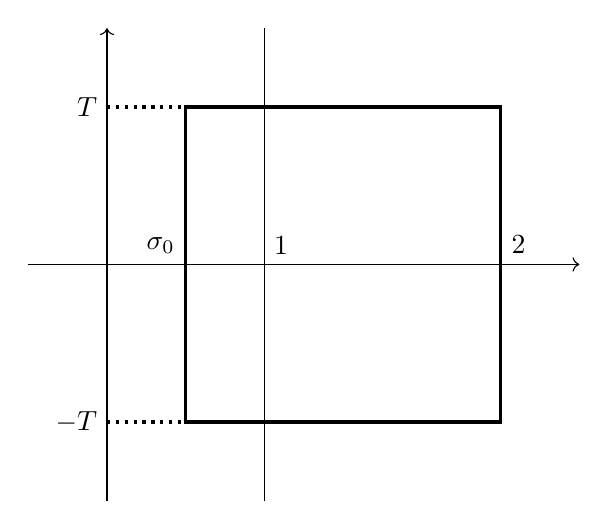
\begin{tikzpicture}
  \draw[->] (-1,0) -- (6,0);
  \draw[->] (0,-3)--(0,-2) node[left]{$-T$} -- (0,2)node[left]{$T$}--(0,3);
  \draw[very thick, dotted] (0,-2) -- (1,-2);
  \draw[very thick, dotted] (0,2) -- (1,2);
  \draw[very thick, black] (1,-2) -- (1,0)node[above left, black]{$\sigma_0$} -- (1,2)
    -- (5,2)--(5,0)node[above right, black]{$2$} -- (5,-2) -- cycle;
      \draw[] (2,-3) -- (2,0)node[above right]{$1$} --(2,3);
\end{tikzpicture}
\end{center}
where $\sigma_0 = 1-\log T$. On the boundary of the rectangle above, we have,
    \begin{enumerate}
      \item $\vert\zeta(s)\vert=O(\log T),T\to\infty$,
      \item $\vert\zeta'(s)\vert = O((\log T)^2)$.
    \end{enumerate}
    \label{lemma_zeta_zeta_derivative_growth_domain}
  \end{lemma}
  \begin{proof}
    Recall that 
    \begin{equation*}
      \zeta'(s) = \sum_{n=1}^\infty {\frac {-\log n} {n^s}}.
    \end{equation*}
    The first statement is due to the first derivative of $\zeta$.  and it is assgined as an exercise. For the second part,
    for $\Re(s),\sigma>1$, we have,
    \begin{align*}
      \zeta(s) & = \sum_{n\geq 1}{\frac 1 {n^s}},\\
      & = \sum_{n\leq T}{\frac 1 {n^s}}+\sum_{n>T}{\frac 1 {n^s}},\\
    \end{align*}
    Using Abel's summation formula by setting $a_n= 1,f(n)={\frac 1 {n^s}}$, we have,
    \begin{align*} 
      \zeta(s) &= \sum_{n=1}^\infty =-s\int_1^\infty {\frac {[t]} {t^{s+1}}}dt,\\
      \sum_{n\leq T}{\frac 1 {n^s}} & = {\frac {[T]} {T^{s}}}-s\int_1^T{\frac {[t]} {t^{s+1}}}dt.
    \end{align*}
    Using this, we get,
    \begin{align*}
      \zeta(s)& = \sum_{n\leq T}{\frac 1 {n^s}}-{\frac {\lfloor T\rfloor} {T^s}}+s\int_1^\infty {\frac {\lfloor t\rfloor} {t^{s+1}}}dt,\\
      & = \sum_{n\leq T}{\frac 1 {n^s}}+{\frac {T^{1-s}} {s-1}} + {\frac {\{ T\}}{T^s}}-s\int_T^\infty {\frac {\{u\}} {u^{s+1}}}du.
    \end{align*}
    Note that the right hand side is analytic where $\Re(s)>0$ and $s\not=1$. Now we will estimate the last equation above on the boundary of the rectangle above.
    \begin{align*}
      \left\vert\sum_{n\leq T}{\frac 1 {n^s}}\right\vert & << \int_1^T{\frac {du} {u^{\Re(s)}}},\\
      &\leq \int_1^T{\frac {du} {u^{\sigma_0}}},\\
      & = {\frac {T^{1-\sigma_0}} {1-\sigma_0}},\\
      &<<\log T.
    \end{align*}
    Observe that ,
    \begin{align*}
      1-\sigma_0  = {\frac 1 {\log T}},T^{1-\sigma_0} = T^{{\frac 1 {\log T}}} = \exp(\log T^{{\frac 1 {\log T}}}) = \exp(1) = e.\\
    \end{align*}
    We also have,
    \begin{align*}
      \left\vert{\frac {T^{1-s}} {s-1}}\right\vert & = {\frac {T^{1-\Re(s)}} {\vert s-1\vert}},\\
      & \leq {\frac {T^{1-\sigma_0}} {\vert s-1\vert}},\\
      & \leq {\frac e {\vert s-1\vert}},\\
      & \leq {\frac e {\sigma_0-1}} =e\log T.
    \end{align*}
    Also consider,
    \begin{align*}
      \left\vert{\frac {\{T\}} {T}}\right\vert \leq {\frac 1 {T^{\Re(s)}}}\leq 1. 
    \end{align*}
    Finally we have,
    \begin{align*}
      \left\vert -s\int_T^\infty {\frac {\{u\}} {u^{s+1}}}du\right\vert& \leq \vert s\vert\int_T^\infty {\frac {du} {u^{\Re(s)+1}}},\\
      & = -{\frac {\vert s\vert} {\Re(s)u^{\Re(s)}}}\bigg{\vert}_T^\infty,\\
      & = {\frac {\vert s\vert} {\Re(s)T^{\Re(s)}}} ,\\
      & \leq {\frac {\vert s\vert} {T^{\Re(s)}}},\\
      & \leq {\frac {\sqrt{2^2+T^2}} {T^{\sigma_0}}},\\
      & << {\frac T {T^{\sigma_0}}} = T^{1-\sigma_0} = e.
    \end{align*}
    For the second part, for $\Re(s)>0,s\not=1$,
    \begin{align*}
      \zeta'(s) = &\sum_{n\leq T}{\frac {-\log n} {n^s}}+{\frac {T^{1-s}(-\log T)} {s-1}}+T^{1-s}{\frac {-1} {(s-1)^2}}\\
      &+{\frac {\{T\}\log T} {T^s}}-\int_T^\infty {\frac {\{u\}} {u^{s+1}}}du + s\int_T^\infty {\frac {\{u\}\log u} {u^{s+1}}}du.
    \end{align*}
    This is obtained simply differentiating the equation,
    \begin{equation*}
      \zeta(s) = \sum_{n\leq T}{\frac 1 {n^s}}+{\frac {T^{1-s}} {s-1}}-{\frac {\{T\}} {T^s}}-s\int_T^\infty {\frac {\{u\}} {u^{s+1}}}du.
    \end{equation*}
    The statement can be shown using all the estimates obtained to show the first part.
  \end{proof}

  \begin{theorem}[Complex Mean Value Theorem]
    Let $f:\Omega\to \C$ be an analytic, where $\Omega$ is a convex open set. Let $a,b\in\Omega$, then there exists $z_1,z_2\in (a,b)$ such that 
    \begin{equation*}
      \Re(f'(z_1)) = \Re\left({\frac {f(b)-f(a)} {b-a}}\right), \Im(f'(z_2)) = \Im\left({\frac {f(b)-f(a)} {b-a}}\right).
    \end{equation*}
    \label{theorem_complex_mean_value}
  \end{theorem}

  \begin{theorem}
    There exist some constants $c_1,c_2$ such that 
    \begin{equation*}
      1 - {\frac {c_1} {(\log T)^9}} \leq \sigma\leq 2\Rightarrow \vert \zeta(s)\vert >{\frac {c_2} {(\log T)^7}},
    \end{equation*}
    where $1<\vert \Im(s)\vert\leq T$. 
    \label{theorem_zeta_modulo_lower_bound}
  \end{theorem}

  \begin{proof}
    We set $z=\sigma+it$ for $\sigma,t\in\R$. Recall Lemma \ref{lemma_analytical_continuation_zeta},
    \begin{equation*}
      \vert\zeta(\sigma)^3\zeta(\sigma+it)^4\zeta(\sigma+2it)\vert\geq 1, \sigma>1.
    \end{equation*}
    Thus we have,
    \begin{equation*}
      \vert\zeta(\sigma+it)\vert^4 \geq\vert\zeta(\sigma)\vert^{-3}\vert\zeta(\sigma+2it)\vert^{-1}\tag{$\ast$}\label{equ_zeta_inequ},
    \end{equation*}
    Consider 
    \begin{equation*}
      \sigma'_0 = 1-{\frac {c_1} {(\log T)^9}},\sigma' = 1+{\frac {c_1} {(\log T)^9}}
    \end{equation*}
    $c_1$ is a positive constant which will be adjusted later.
    \begin{center}
  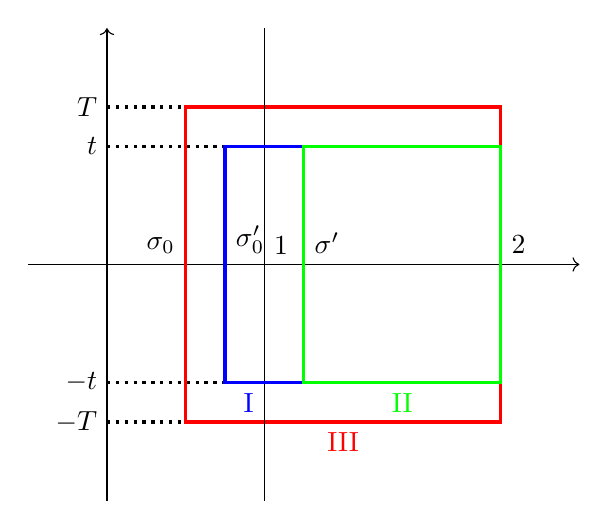
\begin{tikzpicture}
  \draw[->] (-1,0) -- (6,0);
  \draw[->] (0,-3)--(0,-2) node[left]{$-T$}--(0,-1.5)node[left]{$-t$}--(0,1.5)node[left]{$t$} -- (0,2)node[left]{$T$}--(0,3);
  \draw[very thick, dotted] (0,-2) -- (1,-2);
  \draw[very thick, dotted] (0,2) -- (1,2);
  \draw[very thick, dotted] (0,-1.5) -- (1.5,-1.5);
  \draw[very thick, dotted] (0,1.5) -- (1.5,1.5);
  \draw[very thick, red] (1,-2) -- (1,0)node[above left, black]{$\sigma_0$} -- (1,2)
    -- (5,2)--(5,0)node[above right, black]{$2$} -- (5,-2) -- cycle node[midway,below]{III};
      \draw[] (2,-3) -- (2,0)node[above right]{$1$} --(2,3);
      \draw[very thick,  blue] (1.5,-1.5) -- (1.5,0)node[above right, black]{$\sigma'_0$} --(1.5,1.5) -- (2.5,1.5) -- (2.5,-1.5)-- cyclenode[midway,below left]{I};
      \draw[very thick, green] (2.5,-1.5) -- (2.5,0)node[above right,black]{$\sigma'$} --(2.5,1.5)--(5,1.5)--(5,-1.5)--cyclenode[midway,below]{II};
\end{tikzpicture}
\end{center}
    \par Fix the domain II where $\sigma'\leq \sigma\leq 2$, $1\leq\vert t\vert \leq T$.
    \begin{align*}
      \zeta(s) & = {\frac s {s-1}}-s\int_1^\infty {\frac {\{u\}} {u^{s+1}}}du, \Re(s)>0, s\not =1.\\
      \zeta(\sigma) & = {\frac {\sigma-1+1} {\sigma-1}} - \sigma\int_1^\infty {\frac {\{u\}} {u^{\sigma+1}}}du.\\
      & << {\frac 1 {\sigma -1}}\text{ as } \sigma\to 1^+,\\
      \Rightarrow & \zeta(\sigma)^{-1}>>(\sigma-1), \sigma\to 1^{+}
    \end{align*}
    On the domain II, we have, $\sigma'_0<\sigma\leq 2,1\leq \vert t\vert\leq T$. Using Lemma \ref{lemma_zeta_zeta_derivative_growth_domain},
    \begin{equation*}
      \vert\zeta(\sigma+2it)\vert  = O(\log T).
    \end{equation*}
    Substituting these to Equation \eqref{equ_zeta_inequ}, we have,
    \begin{align*}
      \vert \zeta(\sigma+it)\vert^4&>>(1-\sigma)^3(\log T)^{-1},\\
      &>>{\frac {c_1^3} {(\log T)^{27}}}(\log T)^{-1}.\\
      \Rightarrow \vert \zeta(\sigma+it)\vert & >> {\frac {c_1^{{\frac 3 4}}} {(\log T)^7}}\tag{$D1$}\label{eq_ineq_domain_2},
    \end{align*}
    in the domain II.
    \par On the domain I, similarly use Theorem \ref{theorem_complex_mean_value} with 
    \begin{equation*}
      a = \sigma'+it,b=\sigma+it,
    \end{equation*}
    where,
    \begin{equation*}
      1-{\frac {c_1} {(\log T)^9}}\leq \sigma\leq \sigma'.
    \end{equation*}
    We have,
    \begin{equation*}
      {\frac {\zeta(\sigma'+it)-\zeta(\sigma+it)} {\sigma'-\sigma}} = \Re(\zeta(z_1))+\Im(\zeta(z_2)).
    \end{equation*}
    Furthermore,
    \begin{equation*}
      \zeta(\sigma'+it)-\zeta(\sigma+it) = O((\sigma'-\sigma)(\log T)^2).
    \end{equation*}
    By the definition of $\sigma'$, we have,
    \begin{equation*}
      \zeta(\sigma'+it) = \zeta(\sigma+it)+O\left({\frac {c_1} {(\log T)^7}}\right).\tag{$D2$}\label{eq_ineq_domain_1}
    \end{equation*}
    Combining Equations \eqref{eq_ineq_domain_2} and \eqref{eq_ineq_domain_1}, there are some positive constants $A_1,A_2$ such that 
    \begin{align*}
      \vert\zeta(\sigma+it)\vert & \geq \vert\zeta(\sigma'+it)\vert-{\frac {A_1c_1} {(\log T)^7}},\\
      & \geq {\frac {A_2c_1^{{\frac 3 4}}} {(\log T)^7}}-{\frac {A_1c_1} {(\log T)^7}}.
    \end{align*}
    Now take $c_1$ sufficiently small so that in the region,
    \begin{equation*}
      \sigma_0'\leq \sigma\leq \sigma', 1\leq \vert t\vert \leq T,
    \end{equation*}
    we have,
    \begin{equation*}
      \vert\zeta(\sigma+it)\vert \geq {\frac {c_2} {(\log T)^7}}.
    \end{equation*}
    Again combining this with Inequality \eqref{eq_ineq_domain_1}, we obtain the statement.
  \end{proof}
  \begin{corollary}
    \label{corollary_bound_zeta_derivative}
    There exists some constant $c$ such that 
    \begin{equation*}
      {\frac {\zeta'(s)} {\zeta(s)}} = O((\log T)^9),
    \end{equation*}
    for $1-{\frac {c} {(\log T)^9}}\leq \Re(s)\leq 2$ and $1\leq \vert\Im(s)\vert\leq T$.
  \end{corollary}

  \begin{notation}
    Let $c\in\R$ and $f:\C\supseteq\Omega\to \C$. Then we denote,
    \begin{equation*}
      \int_{(c)}f(s)ds = \lim_{T\to\infty}\int_{c-iT}^{c+iT}f(s)ds.
    \end{equation*}
  \end{notation}

  \begin{lemma}
    \label{lemma_y_s_conv}
    \begin{align*}
      {\frac 1 {2\pi i}}\int_{(c)}y^s{\frac {ds} s} = \begin{cases}
        0,\quad(0<y<1),\\
        {\frac 1 2},\quad(y=1),\\
        1,\quad(y>1).
      \end{cases}
    \end{align*}
  \end{lemma}

  \begin{lemma}
    Set,
    \begin{equation*}
      f(s)\defeq  \sum_{n=1}^\infty {\frac {a_n} {n^s}}.
    \end{equation*}
    Suppose this is absolutely convergence in $\Re(s)>c-\varepsilon$ for some $c\in\R,\varepsilon>0$ and $x$ is not an integer, then 
    \begin{equation*}
      \sum_{n<x}a_n = {\frac 1 {2\pi i}}\int_{(c)}f(s){\frac {x^s} s}ds.
    \end{equation*}
    \label{lemma_partial_sum_integration}
  \end{lemma}

  \begin{proof}
    Since $f(s)$ is a limit of a continuous function series which is absolutely convergent on $\Re(s)>c-\varepsilon$, thus this is uniformly convergent in a compact subset of its domain of convergence. Thus we can exchange the integral and the sum namely,
    \begin{equation*}
      {\frac 1 {2\pi i}}\int_{(c)}\left(\sum_{n=1}^\infty {\frac {a_n} {n^s}}\right){\frac {x^s}s}ds = {\frac 1 {2\pi i}}\sum_{n=1}^\infty a_n\int_{(c)}\left({\frac x n}\right)^s{\frac {ds} s}.
    \end{equation*}
    By Lemma \ref{lemma_y_s_conv}, and ${\frac x n}>1\Leftrightarrow n<x$, we derive the statement.
  \end{proof}

  \begin{corollary}
    Let $c>1$ and $x$ be a non-integer, then we have,
    \begin{equation*}
      \psi(x) = {\frac 1 {2\pi i}}\int_{(c)}-{\frac {\zeta'(s)} {\zeta(s)}}{\frac {x^s} s}ds.
    \end{equation*}
    \label{corollary_second_chebyschev_partial_sum}
  \end{corollary}

  \begin{proof}
    From Remark \ref{remark_second_chebyschev_mangoldot},
    \begin{equation*}
    \psi(x)=\sum_{d\leq x}\Lambda(d),
    \end{equation*}
    and by Theorem \ref{theorem_log_zeta_mangoldot} set
    \begin{equation*}
    f(s) = -{\frac {\zeta'(s)} {\zeta(s)}} = \sum_{n=1}^\infty {\frac {\Lambda(n)} {n^s}},
    \end{equation*}
    Thus applying Lemma \ref{lemma_partial_sum_integration}, we get the statement.
  \end{proof}

  \begin{theorem}
    There is a positive constant $c'>0$ such that 
    \begin{equation*}
      \psi(x) = x+O(x\exp(-c'\log(x))).
    \end{equation*}
  \end{theorem}
\setcounter{claim}{0}
  \begin{proof}
    Let $a = 1+{\frac c {\log T}}$ for some $c$ where $T>1$ is sufficiently large and will be chosen later. By Corollary \ref{corollary_second_chebyschev_partial_sum}, we have,
    \begin{equation*}
      \psi(x) = {\frac 1 {2\pi i}}\int_{a-iT}^{a+iT}-{\frac {\zeta'(s)} {\zeta(s)}}{\frac {x^s} s}ds + {\frac 1 {2\pi i}}\int_{(a)}-{\frac {\zeta'(s)} {\zeta(s)}}{\frac {x^s} s}ds- {\frac 1 {2\pi i}}\int_{a-iT}^{a+iT}-{\frac {\zeta'(s)} {\zeta(s)}}{\frac {x^s} s}ds.
    \end{equation*}
    \begin{claim}
     \begin{equation*}
       \left\vert{\frac 1 {2\pi i}}\int_{(a)}-{\frac {\zeta'(s)} {\zeta(s)}}{\frac {x^s} s}ds- {\frac 1 {2\pi i}}\int_{a-iT}^{a+iT}-{\frac {\zeta'(s)} {\zeta(s)}}{\frac {x^s} s}ds\right\vert<\begin{cases}
        x^a\min\{1,T^{-1},\vert\log x\vert^{-1}\},\quad(x\not=1),\\
        {\frac a T},\quad(x=1).
       \end{cases}
     \end{equation*}
    \end{claim}
    \begin{claimproof}
    Exercise.
    %later
    \end{claimproof}
    \par Let 
    \begin{equation*}
      \psi(x) = \underbrace{{\frac 1 {2\pi i}}\int_{a-iT}^{a+iT}-{\frac {\zeta'(s)} {\zeta(s)}}{\frac {x^s} s}ds}_{=I_1} + \underbrace{{\frac 1 {2\pi i}}\int_{(a)}-{\frac {\zeta'(s)} {\zeta(s)}}{\frac {x^s} s}ds- {\frac 1 {2\pi i}}\int_{a-iT}^{a+iT}-{\frac {\zeta'(s)} {\zeta(s)}}{\frac {x^s} s}ds}_{=I_2}.
    \end{equation*}
    Again using Corollary \ref{corollary_second_chebyschev_partial_sum} and the claim, we have,
    \begin{align*}
      I_2 & = {\frac 1 {2\pi i}}\left(\int_{(a)}-\int_{a-iT}^{a+iT}\right)\left(\sum_{n=1}^\infty{\frac {\Lambda(n)} {n^s}}\right){\frac {x^s} s}ds,\\
      & = {\frac 1 {2\pi i}}\sum_{n=1}^\infty \Lambda(n)\left(\left(\int_{(a)}-\int_{a-iT}^{a+iT}\right)\left({\frac x n}\right)^s{\frac {ds} s}\right),\\
      & = \sum_{n=1}^\infty\Lambda(n)O\left(\left({\frac x n}\right)^a\min\left(1,T^{-1}\left\vert\log\left({\frac x n}\right)\right\vert^{-1}\right)\right),\\
      & = O\left(\sum_{n=1}^\infty\Lambda(n)\left({\frac x n}\right)^a\min\left(1,T^{-1}\left\vert\log\left({\frac x n}\right)\right\vert^{-1}\right)\right).
    \end{align*}
    Fix $x$ and let us consider two ranges $\left[{\frac x 2},{\frac {3x} 2}\right]$ and $\left(-\infty,{\frac x 2}\right)\cup\left({\frac {3x} 2},\infty\right)$. 
    If $n$ sits in the second range 
    \begin{equation*}
      {\frac {\log{\frac n x}} {{\frac n x}-1}}\geq 2\log{\frac 3 2}.
    \end{equation*}
    And if $n$ sits in the first interval, we have, 
    \begin{equation*}
      \left\vert\log{\frac x n}\right\vert <<\left\vert{\frac n x}-1\right\vert^{-1}.
    \end{equation*}
    Using this we have,
    \begin{align*}
      \sum_{n\in\left[{\frac x 2},{\frac {3x} 2}\right]}\Lambda(n)\left({\frac x n}\right)^a\min\left(1,T^{-1}\left\vert\log\left({\frac x n}\right)\right\vert^{-1}\right)&<<\sum_{n\in\left[{\frac x 2},{\frac {3x} 2}\right]}\Lambda(n)\left({\frac x n}\right)^a T^{-1}\left\vert{\frac n x}-1\right\vert^{-1}\\
      &<<{\frac {\log x} T}\sum_{n\in\left[{\frac x 2},{\frac {3x} 2}\right]}{\frac 1 {\left\vert {\frac n x}-1\right\vert}}.
    \end{align*}
    Observe that 
    \begin{align*}
      \sum_{n\in\left[{\frac x 2},x\right)}{\frac 1 {{\frac n x}+1}}&<<\int_{{\frac x 2}}^{\lfloor x\rfloor}{\frac {dt} {1-{\frac t x}}},\\
      \sum_{n\in\left(x,{\frac {3x} 2}\right]}{\frac 1 {{\frac n x}-1}}&<<\int^{{\frac {3x} 2}}_{\lceil x\rceil}{\frac {dt} {{\frac t x}-1}}.\\
      \Rightarrow &  \sum_{n\in\left[{\frac x 2},x\right)}{\frac 1 {{\frac n x}+1}}+\sum_{n\in\left(x,{\frac {3x} 2}\right]}{\frac 1 {{\frac n x}+1}}<<x\log x.
    \end{align*}
    Thus we conclude, as $x\to \infty$,
    \begin{equation*}
      \sum_{n\in\left[{\frac x 2},{\frac {3x} 2}\right]}{\frac 1 {\left\vert {\frac n x}-1\right\vert}}<<{\frac {x(\log x)^2} {T}}.
    \end{equation*}
    Let us turn our focus to the second range. We have $\left\vert \log{\frac x n}\right\vert>\log{\frac 3 2}$. Thus 
    \begin{align*}
      \sum_{n<{\frac x 2},{\frac {3x} 2}<n}\Lambda(n)\left({\frac x n}\right)^a\min\left(1,T^{-1}\left\vert\log\left({\frac x n}\right)\right\vert^{-1}\right)&<< {\frac {x^a} T}\sum_{n<{\frac x 2},{\frac {3x} 2}<n}{\frac {\Lambda(n)} {n^a}},\\
      &\leq {\frac {x^a} T}\sum_{n=1}^\infty{\frac {\Lambda(n)} {n^a}}.
    \end{align*}
    Recall that we have,
    \begin{equation*}
      -{\frac {\zeta'(a)} {\zeta(a)}} = \sum_{n=1}^\infty {\frac {\Lambda(n)} {n^a}}.
    \end{equation*}
    Using Theorem \ref{thorem_zeta_zeta_derivatie_residue}, we see, as $a\to1^+$,
    \begin{equation*}
      \left\vert{\frac {\zeta'(a)} {\zeta(a)}}\right\vert<<{\frac 1 {a-1}}.
    \end{equation*}
    Using Corollary \ref{corollary_bound_zeta_derivative}, we see,
    \begin{equation*}
      {\frac {x^a} T}{\frac 1 {a-1}}<<{\frac {x^a} {T}}(\log T)^9.
    \end{equation*}
    Combining all, we derive,
    \begin{equation*}
      \psi(s)={\frac 1 {2\pi i}}\int_{a-iT}^{a+iT}{\frac {-\zeta'(s)} {\zeta(s)}}{\frac {x^s} s}ds+O\left({\frac {x(\log x)^2} {T}}+{\frac {x^a} T}(\log T)^9\right).
    \end{equation*}
    \par Recall Cauchy's Residue theorem, suppose $f:\Omega\to\C$ is meromorphic where $\Omega$ is simply connected with poles $a_i,1\leq i\leq n$ poles in $U\subseteq\Omega$ where the boundary of $U$ is a simple closed curve $\gamma$. Then,
    \begin{equation*}
      {\frac 1 {2\pi i}}\int_\gamma f(s)ds = \sum_{i=1}^n \Res(f,a_i)+\constant.
    \end{equation*}
    Consider the following closed path $R_T$ which we traverse counterclockwise.
    \begin{center}
  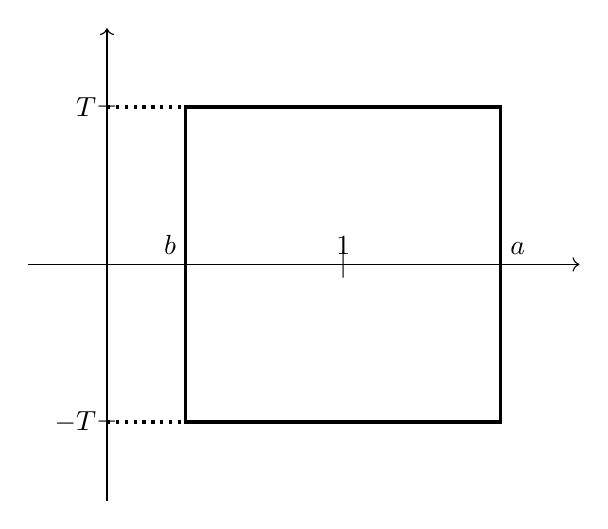
\begin{tikzpicture}
  \draw[->] (-1,0) -- (6,0);
  \draw[->] (0,-3) -- (0,3);
  \draw[very thick, dotted] (0,2)node[left]{$T$}--(1,2);
  \draw[very thick, dotted] (0,-2)node[left]{$-T$}--(1,-2);
  \draw (0,2)node{$-$};
  \draw (0,-2)node{$-$};
  \draw[very thick] (1,-2) -- (1,2)
    -- (5,2) -- (5,-2) -- cycle;
  \draw (1,0)node[above left]{$b$};
  \draw (5,0)node[above right]{$a$};
\draw (3,0)node{$|$};
\draw (3,0)node[above]{$1$};
\end{tikzpicture}
\end{center}
%Current current
\par where $a = 1+{\frac c {(\log(T))^9}},b = 1-{\frac c {(\log(T))^9}}$ $\Re(s)>0,s\not=1$. %$\Re(s)>b$.
We claim that ${\frac {\zeta'(s)} {\zeta(s)}}$ can be analytically continued to $\Re(s)\geq b$ except simple pole at $s=1$ with residue $-1$. By Theorem \ref{thorem_zeta_zeta_derivatie_residue} and Theorem \ref{theorem_zeta_modulo_lower_bound}, we obtain
\begin{align*}
  {\frac 1 {2\pi i}}\int_{R_T}{\frac {-\zeta'(s)} {\zeta(s)}}{\frac {x^s} s}ds & = \Res_{s=1}\left({\frac {-\zeta'(s)} {\zeta(s)}}{\frac {x^s} s}\right),\\
  & = x.
\end{align*}
\par Now consider $R_T$ which is the closed path.
\begin{equation*}
  \int_{R_T} = \int_{a-iT}^{a+iT}+\int_{a+iT}^{b+iT}+\int_{b+iT}^{b-iT}+\int_{b-iT}^{a-iT}.
\end{equation*}
We then have,
\begin{equation*}
  {\frac 1 {2\pi i}}\int_{a-iT}^{a+iT} {\frac {-\zeta'(s)} {\zeta(s)}}{\frac {x^s} {s}}ds = x -{\frac 1 {2\pi i}}\left(\int_{a+iT}^{b+iT}+\int_{b+iT}^{b-iT}+\int_{b-iT}^{a-iT}\right) {\frac {-\zeta'(s)} {\zeta(s)}}{\frac {x^s} {s}}ds 
\end{equation*}
\begin{align*}
  \left\vert{\frac 1 {2\pi i}}\int_{a+iT}^{b+iT}{\frac {-\zeta(s)}{\zeta(s)}}{\frac {x^s} {s}}ds\right\vert &= \left\vert{\frac 1 {2\pi i}}\int_a^b{\frac {-\zeta(u+iT)}{\zeta(u+iT)}}{\frac {x^{(u+iT)}} {(u+iT)}}du\right\vert,\\
  & <<\int_a^b\left\vert{\frac {-\zeta'(u+iT)} {\zeta(u+iT)}}\right\vert{\frac {x^u} {\vert u+iT\vert}}du,\quad(\vert u+iT\vert^2\geq1)\\
  &\stackrel{\text{Theorem \ref{theorem_zeta_modulo_lower_bound}}}{<<}{\frac {\log^9T} T}x^a\int_b^a du,\\
  &<<{\frac {x^a} T}.
\end{align*}
Now we have,
\begin{align*}
  \left\vert\int_{b-iT}^{b+iT}{\frac {-\zeta'(s)} {\zeta(s)}}{\frac {x^s} {s}}ds\right\vert & = \left\vert{\frac 1 {2\pi}}\int_{-T}^T{\frac {\zeta'(b+iu)} {\zeta(b+iu)}}{\frac {x^{b+iu}} {b+iu}}du\right\vert,\\
  & << \log^9T\int_{-T}^T{\frac {x^b} {\sqrt{b^2+u^2}}}du,\\
  &<< x^b\log^9T\int_{0}^T{\frac {du} {\sqrt{b^2+u^2}}}du,\\
  & << x^b\log^9T\int_1^T{\frac {du} u},\\
  & = x^b\log^{10}T.
\end{align*}
Now back to the beginning,
\begin{equation*}
  \psi(x) = x+O\left({\frac {x^a} {T}}+x^b\log^{10}T\right)+O\left({\frac {x\log^2x} T}+{\frac {x^a} T}\log^9T\right).
\end{equation*}
Choose $T$ to be such that $2c\log x = \log^{10}T,x=e^{{\frac {\log^{10}T} {2c}}}$.
\begin{align*}
  x^{{\frac c {\log^9T}}}&=e^{{\frac {\log T} 2}}  = \sqrt{T}.\\
  x^{1-{\frac c {\log^9 T}}}&\cdot\log^{10}T+{\frac {x\log^2 x} T}+{\frac {x^{1+{\frac c {\log^{9}T}}}} {T}}\log^9T&\\
  & = x\cdot T^{-{\frac 1 2}}\log^{10} T+{\frac {x\log^2 x} T}\\
  &+x{\frac {\sqrt{T}} T}\log^{10}T\left({\frac x {\sqrt{T}}}\right)(\log^{10}T + {\frac {\log^2x}{\sqrt{x}}}+\log^9T),\\
  &<<{\frac x {T^s}}=xe^{-c(\log x)^{{\frac 1 {10}}}}.
\end{align*}
%later
  \end{proof}
  %12/11
\begin{definition}[Gamma function] We define the Gamma function $\Gamma:\C\to\C$ as
  \begin{equation*}
    \Gamma(s)\defeq \int_0^\infty t^{s-1}e^{-t}dt, \sigma>0.
  \end{equation*}
\end{definition}
\begin{remark}
  Suppose $\Re(s) = \sigma$ then,
  \begin{align*}
    \vert\Gamma(s)\vert &\leq \int_0^\infty \vert t^{s-1}\vert e^{-t}dt,\\
    & = \int_0^\infty t^{\sigma-1}e^{-t}dt,\\
    & = \left(\int_0^1+\int_1^\infty\right)t^{\sigma-1}e^{-t}dt,\\
    &\leq \int_0^1t^{\sigma-1}dt + \int_1^\infty t^{\sigma-1}e^{-t}dt, \left({\frac {t^n} {e^t}}\stackrel{t\to\infty}{\to}0\right).\\
    &<< {\frac 1 \sigma}+\int_1^\infty t^{\sigma-1}t^{-2\sigma}dt,\\
    &<< {\frac 1 \sigma}.
  \end{align*}
  \label{remark_bound_gamma}
\end{remark}

\begin{theorem}
  \begin{equation*}
    F(s) = \int f(s,t)dt.
  \end{equation*}
  $F:\Omega\to \C$ is analytic in $\Omega$ if 
  \begin{enumerate}[i).]
    \item $f(s,t)$ is continuous in $(s,t)$,
    \item $f(s,t)$ is analytic in $s$,
    \item $\int f(s,t)$ is uniformly bounded on compact subsets of $\Omega$.
  \end{enumerate}
\end{theorem}
In Remark \ref{remark_bound_gamma}, suppose $a\leq\Re(s)\leq b$ then the last two inequalities will be,
\begin{align*}
  \int_0^1t^{\sigma-1}dt + \int_1^\infty t^{\sigma-1}e^{-t}dt&\\
    &<<_b {\frac 1 \sigma}+\int_1^\infty t^{b-1}t^{-2b}dt,\\
    &<<_b {\frac 1 \sigma}+{\frac 1 b} = {\frac 1 a}+{\frac 1 b}.
\end{align*}
Thus we observe that in $\sigma>0$, using integration by parts,
\begin{align*}
  \Gamma(s+1) & = s\Gamma(s).
\end{align*}
Thus for any $n\in\N$, we have $\Gamma(n) = n!$.
We have,
\begin{equation*}
  \Gamma(s) = {\frac {\Gamma(s+1)} s},\sigma>0.
\end{equation*}
Note $\Gamma(s+1)$ is analytic if $\sigma>-1$. Thus $\Gamma(s)$ is analytic in $\sigma>-1$ except simple pole at $s=0$ with residue $1$. That is 
\begin{equation*}
  \lim_{s\to0}s\Gamma(s) = 1. 
\end{equation*}
We also have,
\begin{equation*}
  \Gamma(s) = {\frac {\Gamma(s+2)} {\Gamma(s+1)}},\sigma>0.
\end{equation*}
Note that in the numerator, we have $\sigma>-2$. $\Gamma(s)$ is analytic when $\sigma>-2$ except simple poles at $s=0,-1$ with residue 
\begin{align*}
  \lim_{s\to-1}(s+1)\Gamma(s) = {\frac {\Gamma(-1)} {-1}} = -1.
\end{align*}
Iterating the process, we have the following theorem,
\begin{theorem}
  \label{theorem_analytic_continuation_gamma}
  $\Gamma(s)$ can be analytically continued to $\C$ except simple poles at $s = -k$ where $k\in\Z_{\geq 0}$ with residue ${\frac {(-1)^k} {k!}}$.
\end{theorem}
\begin{remark}
  \begin{align*}
    \Gamma(s)\Gamma(1-s) & = {\frac {\pi} {\sin\pi s}}, s\in\C.\\
    \lim_{s\to m}\Gamma(s)\Gamma(1-s)\sin\pi s &= \pi.\\
    \Gamma(s)\Gamma\left(s+{\frac 1 2 }\right) &= \sqrt{\pi}2^{1-2s}\Gamma(2s),\forall s\in\C.
  \end{align*}
  \label{remark_gamma_poles}
\end{remark}
\begin{exercise}
  Show 
  \begin{equation*}
     \forall \alpha\in \R, x>0, \sum_{n\in\Z}e^{-(n+\alpha){\frac \pi x}}=\sqrt{x}\sum_{n\in\Z}e^{-n^2\pi x+2\pi i n \alpha}.
  \end{equation*}
  Note that $\sum_{n\in\Z}a_n$ is convergent if 
  \begin{equation*}
    s_N\defeq \sum_{\vert n\vert \leq N}a_n,
  \end{equation*}
  is convergent.
  \label{exercise_fourier_poisson_summation}
\end{exercise}
\begin{theorem}
  Let $\sigma>1$ and $F\in L^1(\R)$, ie $F:\R\to\C$ and 
  \begin{equation*}
    \int_{-\infty}^\infty \vert F(t)\vert dt<\infty.
  \end{equation*}
  We have,
  \begin{equation*}
    \sum_{n\in\Z}F(n+u)
  \end{equation*}
  is absolutely and uniformly convergent in $u$. Also we have,
  \begin{equation*}
    \sum_{n\in\Z}\vert \hat{F}(n)\vert\leq\infty,
  \end{equation*}
  then 
  \begin{equation*}
    \sum_{n\in\Z}F(n+u) = \sum_{n\in\Z}\hat{F}(n)e^{2\pi i n u}.
  \end{equation*}
  \label{theorem_fourier_transform_convergent}
\end{theorem}
\begin{proof}
  Use Exercise \ref{exercise_fourier_poisson_summation}.
\end{proof}
\begin{theorem}
  \label{theorem_gamma_singulality}
  $\Gamma(s) \not=0,\forall s\in\C$.
\end{theorem}
\begin{proof}
  Note that the case when $s\in\Z$ is already shown. Thus suppose $s\not\in\Z$. Suppose $\Gamma(s)=0$, then it will follow that $\Gamma(1-s)$ by Remark \ref{remark_gamma_poles}. But this is a contradiction to Theorem \ref{theorem_analytic_continuation_gamma} as it has a pole at non-integer point.
  Similarly from Remark \ref{remark_gamma_poles}, we see that ${\frac 1 {\Gamma(s)}}$ has a simple zero at $s=0,-1,-2,\cdots$.
  \par By definition, consider,
  \begin{equation*}
    \Gamma\left({\frac s 2}\right) = \int_0^\infty e^{-t}t^{{\frac s 2}-1}dt, \sigma>0.
  \end{equation*}
  Replace $t=n^2\pi x,dt = n^2\pi dx$, we get,
  \begin{align*}
    \pi^{{\frac {-s} 2}}\Gamma\left({\frac s 2}\right)n^{-s} & = \int_0^\infty x^{{\frac s 2}-1}e^{-n^2\pi x}dx, \sigma>1.\\
    \pi^{{\frac {-s} 2}}\Gamma\left({\frac s 2}\right)\zeta(s) & = \sum_{n\in\N}\int_0^\infty x^{{\frac s 2}-1}e^{-n^2\pi x}dx,\\
    & = \int_0^\infty x^{{\frac s 2}-1}\left(\sum_{n\in\N}e^{-n^2\pi x}\right)dx,\\
    & = \sum_{n\in\N}\int_0^\infty\vert x^{{\frac s 2}-1}e^{-n^2\pi x}\vert dx,\\
    & = \sum_{n\in\N}\left(\int_0^\infty x^{{\frac \sigma 2}-1}e^{-n^2\pi x}dx\right),\\
    & = \sum_{n=1}^\infty \pi^{-{\frac {\sigma} 2}}\Gamma\left({\frac \sigma 2}\right)n^{-\sigma},\\
    & = \pi^{-{\frac \sigma 2}}\Gamma\left({\frac \sigma 2}\right)\zeta(s),\sigma>1,\\
    & < \infty.\\
    \pi^{-{\frac s 2}}\Gamma\left({\frac s 2}\right)\zeta(s) & = \int_0^\infty x^{{\frac s 2}-1}\left(\sum_{n\in\N}e^{-n^2\pi x}\right).
  \end{align*}
  Using Exercise \ref{exercise_fourier_poisson_summation} and set $\alpha=0$, we have,
  \begin{align*}
    \sum_{n\in\Z}e^{-n^2{\frac \pi s}} & = \sqrt{s}\sum_{n\in\Z}e^{-n^2 \pi x}.\\
    \sum_{n\in\Z}e^{-n^2\pi x}& << \sum_{n\in\N}e^{-n\pi x},\\
    & << \int_1^\infty e^{-\pi xt }dt,\\
    & << {\frac {e^{-\pi x}} {x}}, x>0.
  \end{align*}
  Set $\theta(x)\defeq  \sum_{n\in\Z}e^{n^2\pi x}$ then,
  \begin{align*}
    \theta(x) &= 1+2\sum_{n\in\N}e^{-n^2\pi x}.\\
    \sum_{n\in\N}e^{-n^2\pi x}&= {\frac {\theta(x) - 1} 2}, x>0.
  \end{align*}
  Using the exercise, we have,
  \begin{equation*}
    \theta\left({\frac 1 x}\right) = \sqrt{x}\theta(x).
  \end{equation*}
  Set $w(x) \defeq {\frac {\theta(x)-1} 2}$. Thus write
  \begin{align*}
    w\left({\frac 1 x}\right) & = {\frac {\theta\left({\frac 1 x}\right)-1} 2},\\
    & = {\frac {\sqrt{x}\theta(x) - 1} 2},\\
    & = {\frac {\sqrt{x}\theta (x)-1} {2}}.\\
    w\left({\frac 1 x}\right)&= \sqrt{x}w(x)+{\frac {\sqrt{x}} 2}-{\frac 1 2}. \\
    \pi^{-{\frac 1 2}}\Gamma\left({\frac s 2}\right)\zeta(s) &= \int_0^\infty x^{{\frac s 2}-1}w(x)dx, \sigma>1.
  \end{align*}
  \par Step 3
  \begin{align*}
    \int_0^1 x^{{\frac s 2}-1}w(x)dx+\int_1^\infty x^{{\frac s 2}-1}w(x)dx.
  \end{align*}
  Taking $x = {\frac 1 y}$ and $dx = -{\frac 1 {y^2}}dy$ we have,
  \begin{align*}
    \int_1^\infty \left({\frac 1 {y^2}}\right)^{{\frac s 2}-1}w\left({\frac 1 y}\right){\frac {-1} {y^2}}dy & = \int_1^\infty y^{-{\frac s 2}}w\left({\frac 1 y}\right){\frac {dy} y},\\
    & = \int_1^\infty y^{-{\frac 1 2}}\left(\sqrt{y}w(y)+{\frac {\sqrt{y}} 2}-{\frac 1 2}\right){\frac {dy} y},\\
    & = \int_1^\infty y^{-{\frac s 2}+{\frac 1 2}}w(y){\frac {dy} y}+\int_1^\infty {\frac {y^{-{\frac s 2}+{\frac 1 2} -1 }} 2}dy - {\frac 1 2}\int_1^\infty y^{-{\frac s 2}-1}dy,\\
    & = \int_1^\infty y^{{\frac {1-s} 2}}w(y){\frac {dy} y}+{\frac 1 {s(s-1)}}+\int_1^\infty (x^{{\frac s 2}}+x^{\frac {1-s} 2})w(x){\frac {dx} x},\sigma>1.
  \end{align*}
  \par Step 4, 
  \begin{align*}
    \int_1^\infty \vert x^{{\frac s 2}}+x^{{\frac {1-s} 2}}\vert \vert w(x)\vert {\frac {dx} x} &\leq \int_1^\infty (x^{{\frac {\sigma 2}-1}}+x^{{\frac {1-\sigma} 2}-1})\vert w(x)\vert dx,\\
    &<< \int_1^\infty {\frac {(x^{{\frac \sigma 2}-1}+x^{{\frac {1-\sigma} 2}-1})} {e^{\pi x}}}dx,\sigma\in\R,\\
    &<< \int_1^\infty {\frac {e^x} {e^{\pi x}}}dx,
    & << 1.
  \end{align*}
  $\int_1^\infty \vert x^{{\frac s 2}}+x^{{\frac {1-s} 2}}\vert \vert w(x)\vert {\frac {dx} x}$ is analytic in $\C$. 
  \begin{align*}
    s(s-1)\pi^{-{\frac s 2}}\Gamma\left({\frac s 2}\right)\zeta(s) & = 1+s(s-1)\int^\infty_1(x^{{\frac s 2}} +x^{{\frac {1-s} 2}})w(x){\frac {dx} x}.
  \end{align*}
  Set $\xi(x) \defeq 1+s(s-1)\int^\infty_1(x^{{\frac s 2}} +x^{{\frac {1-s} 2}})w(x){\frac {dx} x}$, then it is entire. and for all $s$ we have,
  \begin{equation*}
    \xi(1-s)=\xi(s).
  \end{equation*}
  Thus obtain,
  \begin{equation*}
    (1-s)(1-s-1)\pi^{-{\frac {(1-s)} 2}}\Gamma\left({\frac {1-s} 2}\right) = s(s-1)\pi^{-{\frac s 2}}\Gamma\left({\frac s 2}\right)\zeta(s).
  \end{equation*}
  Using the construction of $w(s)$ we have,
  \begin{equation*}
    \vert w(x)\vert <<\vert \theta(x)\vert << {\frac {e^{-\pi x}} x},\forall x>0.
  \end{equation*}
  Also we have,
  \begin{align*}
    \zeta(1-s)&= \pi^{-s+{\frac 1 2}}{\frac {\Gamma\left({\frac s 2}\right)} {\Gamma\left({\frac {1-s} 2}\right)}}\zeta(s),\\
    \zeta(1-s) & = \pi^{-s}2^{1-s}\cos\left({\frac {\pi s} s}\right)\Gamma(s)\zeta(s).
  \end{align*}
  Note that $\zeta(s)$ has an analytic continuation to $\C$ except simple pole at $s$.
  %Missing part below
  \begin{align*}
    \lim_{s\to 1}\zeta(1-s) &= \pi^{-1}\lim_{s\to 1}{\frac {\cos{\frac {\pi s} 2} \zeta(s)(s-1)} {s-1}}.\\
    \lim_{s\to 1}{\frac {\cos{\frac {\pi s} 2}} {s-1}} & = \lim_{s\to 0}{\frac {\cos\left({\frac \pi 2}(1-s)\right)} {-s}},\\
    & = \lim_{s\to0}{\frac {\sin{\frac \pi 2}s} {-s\cdot{\frac \pi 2}}}{\frac \pi 2},\\
    & = -{\frac \pi 2}.\\
    \Rightarrow& \lim_{s\to 1}\zeta(1-s) = -{\frac 1 2}.
  \end{align*}
  \begin{align*}
    \zeta(-2n) & = \pi^{-(2n+1)}2^{1-2n-1}\cos\left({\frac \pi 2}(2n+1)\right)\Gamma(2n+1)\zeta(2n+1)=0.
  \end{align*}
  Recall \begin{align*}
  \zeta(s) & = \sum_{n\in\N}{\frac 1 {n^s}},\\
  & = {\frac s {s-1}}-s\int_1^\infty {\frac {\{t\}} {t^{s+1}}}dt, \sigma>0,s\not=1.
  \end{align*}
  If $s$ is real,
  \begin{align*}
  \left\vert \zeta(s)-{\frac s {s-1}}\right\vert &\leq \vert s\vert\int_1^\infty {\frac {\{t\}} {t^{\sigma+1}}}dt,\\
  & < {\frac {\vert s\vert }\sigma} = {\frac \sigma \sigma}=1.
  \end{align*}
  Thus we obtain,
  \begin{align*}
  -1+{\frac s {s-1}}&<\zeta(s)<1+{\frac s {s-1}}\\
    {\frac 1 {s-1}}&<\zeta(s)<{\frac {2s-1} {s-1}},\\
    -1<(1-s)\zeta(s)&<1-2s<0\quad\text{ if } {\frac 1 2}<s<1\\
    \Rightarrow & \zeta(s)\not=0,\quad \text{ if } {\frac 1 2}<s<1.
  \end{align*}
  %later
\end{proof}
%1218


%Missing above,
\subsection{Primitive characters}
Suppose $q_0|q$. Then we have a natural map 
\begin{equation*}
  \Z/q\Z\to \Z/q_0\Z
\end{equation*}

\begin{definition}
  Let $\chi\tmod{q}$ be a character and $q_0|q$. If there exists a character $\chi^*\tmod{q_0}$ making the following diagram commutative, 
  \begin{center}
    \begin{tikzcd}
(\Z/q\Z)^\times \arrow[d, "f"'] \arrow[r, "\chi"] & \C^\times \\
(\Z/q_0\Z)^\times \arrow[ru, "\chi^*"']           &          
\end{tikzcd}
  \end{center}
  we say $\chi$ factors through $(\Z/q_0\Z)$ or $\chi^*$ induces $\chi$. If $q_0$ is minimal among positive such numbers, we say $q_0$ is a conductor of $\chi$.
\end{definition}

\begin{definition}
  A character $\chi\tmod{q}$ is called primitive if its conductor is $q$ only. Otherwise the character is imprimitive. 
\end{definition}

\begin{example}
  Take $\chi:(\Z/8\Z)^\times\to\C^\times$ such that 
    \begin{center}
\centering
\begin{tabular}{l|l}
$n$ & $\chi(n)$ \\ \hline
$1$ & $1$       \\
$3$ & $-1$      \\
$5$ & $1$       \\
$7$ & $-1$     
\end{tabular}
\end{center}
Then $4$ is a conductor with $\chi^*:(\Z/4\Z)^\times\to\C^\times$,
    \begin{center}
\centering
\begin{tabular}{l|l}
$n$ & $\chi^*(n)$ \\ \hline
$1$ & $1$       \\
$3$ & $-1$       
\end{tabular}
\end{center}
\end{example}

\begin{example}
  Take $\chi:(\Z/6\Z)^\times\to\C^\times$ such that 
    \begin{center}
\centering
\begin{tabular}{l|l}
$n$ & $\chi(n)$ \\ \hline
$1$ & $1$       \\
$5$ & $-1$       \\
\end{tabular}
\end{center}
Then $3$ is a conductor with $\chi^*:(\Z/3\Z)^\times\to\C^\times$,
    \begin{center}
\centering
\begin{tabular}{l|l}
$n$ & $\chi^*(n)$ \\ \hline
$1$ & $1$       \\
$2$ & $-1$       
\end{tabular}
\end{center}
\end{example}

\begin{remark}
  All principal characters $\tmod {q}$ for $q>1$ are imprimitive by construction.
\end{remark}

We set as usual $s=\sigma+it$ for $\sigma,t\in\R$. 

\begin{lemma}
  Suppose $\chi\tmod q$ is induced by $\chi^*\tmod q_0$. We then have,
  \begin{equation*}
    \sigma>1\Rightarrow L(s,\chi) = L(s,\chi^*)\prod_{p\mid q}\left(1-{\frac {\chi^*(p)} {p^s}}\right).
  \end{equation*}
  \label{lemma_induced_character_L}
\end{lemma}

\begin{proof}We know that for $\sigma>1$,
  \begin{equation*}
    L(s,\chi) = \prod_{p\nmid q}\left(1-{\frac {\chi(p)} {p^s}}\right)^{-1}.
  \end{equation*}
  Also 
  \begin{align*}
    L(s,\chi^*) &= \prod_{p\nmid q_0}\left(1-{\frac {\chi(p)} {p^s}}\right)^{-1},\\
    & = \prod_{\substack{p\nmid q_0\\p\nmid q}}\left(1-{\frac {\chi^*(p)} {p^s}}\right)^{-1}\prod_{\substack{p\nmid q_0\\p\mid q}}\left(1-{\frac {\chi^*(p)} {p^s}}\right)^{-1},\\
    & = L(s,\chi)\prod_{\substack{p\nmid q_0\\p\mid q}}\left(1-{\frac {\chi^*(p)} {p^s}}\right)^{-1}.
  \end{align*}
\end{proof}

\begin{remark}
  Using Identity theorem, Lemma \ref{lemma_induced_character_L} holds for all $s\in \C$.
\end{remark}

\begin{lemma}
  Suppose $x\in\left[0,{\frac 1 2}\right]$, then 
  \begin{equation*}
    \vert\sin\pi x\vert\geq 2x.
  \end{equation*}
  \label{lemma_sin_lower_bound}
\end{lemma}

\begin{proof}
  Exercise.
\end{proof}

\begin{definition}[Gauss sum]
  Let $\chi\tmod q$ be a character. The Gauss sum is,
  \begin{equation*}
    \tau(\chi)\defeq\sum_{k=1}^q\chi(k)e^{{\frac {2\pi ki} q}}.
  \end{equation*}
\end{definition}

\begin{lemma}
  For $n\in \Z$, we have,
  \begin{equation*}
    \chi(n)\tau(\overline{\chi}) = \sum_{k=1}^q \overline{\chi}(k)e^{{\frac {2\pi i kn} q}},
  \end{equation*}
  where $\chi$ is a primitive character modulo $q$ and $\chi\not=\chi_0$. 
  \label{lemma_gauss_sum_character}
\end{lemma}
\begin{theorem}
  If $\chi\tmod q$ is primitive then,
  \begin{equation*}
    \vert\tau(\chi)\vert = \sqrt{q}.
  \end{equation*}
  \label{theorem_gauss_sum_primitive}
\end{theorem}
\begin{proof}
By Lemma \ref{lemma_gauss_sum_character}, we have,
  \begin{align*}
    \chi(n)\tau(\overline{\chi}) &= \sum_{k=1}^q \overline{\chi}(k)e^{{\frac {2\pi i k} q}},\\
    \overline{\chi(n)}\overline{\tau(\overline{\chi})} &= \sum_{l=1}^q\chi(l)e^{-{\frac {2\pi i l} q}}.
  \end{align*}
  Multiplying this equation with the one in the statement we have,
  \begin{equation*}
    \vert \chi(n)\vert^2\vert \tau(\overline{\chi})\vert^2 = \sum_{k,l=1}^q \overline{\chi(k)}\chi(l)e^{{\frac {2\pi i (k-l)} q}}.
  \end{equation*}
  Applying $\sum_{n=1}^q$ to the both sides of the above equation, we have,
  \begin{align*}
    \vert\tau(\overline{\chi})\vert^2\sum_{n=1}^q\vert\chi(n)\vert^2 = \sum_{k,l=1}^q\overline{\chi(k)}\chi(l)\left(\sum_{n=1}^q\left(e^{{\frac {2\pi i(k-l)} q}}\right)^n\right).
  \end{align*}
  Note that 
  \begin{align*}
    x+x^2+\cdots+x^q &= \begin{cases}
      {\frac {x(x^q-1)} {x-1}},\quad(x\not =1),\\
      q,\quad(x=1),
    \end{cases}\\
    & = \begin{cases}
      0,\quad(x\not =1, x^q = 1),\\
      q,\quad(x=1),
    \end{cases}
  \end{align*}
  Take $x = e^{{\frac {2\pi i (k-l)} q}} = \cos{\frac {2\pi} q}(k-l)+i\sin{\frac {2\pi} q}(k-l)=1$. $x=1$ if and only if $q|k-l$ thus 
  \begin{equation*}
    \sum_{n=1}^q\left(e^{{\frac {2\pi i(k-l)} q}}\right)^n = \begin{cases}
      0,\quad(q\nmid k-l),\\
      q,\quad(\text{otherwise}).
    \end{cases}
  \end{equation*}
  Therefore, we get,
  \begin{align*}
    \vert\tau (\overline{\chi})\vert^2\sum_{n=1}^q\vert\chi(n)\vert^2 & = q\sum_{\substack{k,l=1\\ q|k-l}}^q \overline{\chi}(k)\chi(l),\\
    & = q\sum_{k=1}^q\overline{\chi}(k)\chi(k),\\
    & = q\sum_{k=1}^q \vert \chi(k)\vert^2.
  \end{align*} 
\end{proof}
\begin{theorem}[Pólya-Vinogradov]$\:$\\
  Let $\chi\tmod q$ be a primitive character. We have,
  \begin{equation*}
    \left\vert\sum_{n\leq x}\chi(n)\right\vert<<\sqrt{q}\log q.
  \end{equation*}
  This inequality is uniform in $q$.
\end{theorem}
\begin{proof}
  \par Consider $(n,q)=1$, then 
  \begin{align*}
    \chi(n)\tau(\overline{\chi}) & = \chi(n)\sum_{k=1}^q\overline{\chi}(k)e^{{\frac {2\pi i k} q}},\\
    & = \chi(n)\sum_{\substack{k=1\\(k,q)=1}}^q\overline{\chi}(k)e^{{\frac {2\pi i k} q}},\\
  \end{align*}
  Set $k = nt$, we get,
  \begin{align*}
    \chi(n)\tau(\overline{\chi}) & = \sum_{\substack{t=1\\ (t,q)=1}}^q\overline{\chi}(nt)\chi(n)e^{{\frac {2\pi i nt} q}}.\\
    \overline{\chi}(nt) & = \overline{\chi}(n)\overline{\chi}(t).\\
    \chi(n)\tau(\overline{\chi}) & = \sum_{\substack{t=1\\ (t,q)=1}}^q\overline{\chi}(t)e^{{\frac {2\pi i nt} q}}.
  \end{align*}
  Observe that 
  \begin{align*}
    \tau(\overline{\chi})\left(\sum_{n\leq x}\chi(n)\right) & = \sum_{k=1}^{q-1}\overline{\chi}(k)\left(\sum_{n\leq x}e^{{\frac {2\pi i kn} q}}\right),\\
    \vert\tau(\overline{\chi})\vert\cdot\left\vert\sum_{n\leq x}\chi(n)\right\vert & \leq \sum_{k=1}^{q-1}\left\vert\sum_{n\leq x}e^{{\frac {2\pi i kn} q}}\right\vert,\\
    & = \sum_{k=1}^{q-1}\left\vert{\frac {e^{{\frac {2\pi i k} q}}\left(e^{{\frac {2\pi in[x]} q}}-1\right)} {e^{{\frac {2\pi i k} q}} - 1}}\right\vert,\\
    &\leq \sum_{k=1}^{q-1}{\frac 2 {\vert e^{{\frac {2\pi k} q}}-1\vert}},\\
  \end{align*}
  Note that for all $y\in \R$,
  \begin{align*}
    2 i\sin y &= e^{-iy}(e^{2iy}-1),\\
    \vert 2\sin y\vert & = \vert e^{2iy}-1\vert.
  \end{align*}
  Apply this to the equation above we have,
  \begin{equation*}
    \sum_{k=1}^{q-1}{\frac 2 {\vert e^{{\frac {2\pi k} q}}-1\vert}} = \sum_{k=1}^{q-1}{\frac 1 {\vert\sin{\frac {\pi k} q}\vert}}.
  \end{equation*}
  Using Lemma \ref{lemma_sin_lower_bound}, we get,
  \begin{align*}
    \sum_{k=1}^{q-1}{\frac 1 {\vert\sin{\frac {\pi k} q}\vert}} & = \sum_{1\leq k\leq{\frac q 2}}{\frac 1 {\vert\sin{\frac {\pi k} q}\vert}}+\sum_{{\frac q 2}<k}^{q-1}{\frac 1 {\vert\sin{\frac {\pi k} q}\vert}},\\
    & = 2\sum_{1\leq k\leq{\frac q 2}}{\frac 1 {\vert\sin{\frac {\pi k} q}\vert}},\\
    &\leq \sum_{1\leq k\leq{\frac q 2}}{\frac k q} << q\log{\frac q 2}<<q\log q.
  \end{align*}
  Recall Theorem \ref{theorem_gauss_sum_primitive}, we have $\vert\tau(\chi)\vert=\sqrt{q}$ as $\chi$ is primitive. Therefore, for $q>1$, we have,
  \begin{equation*}
    \left\vert\sum_{n\leq x}\chi(n)\right\vert<<\sqrt{q}\log q,
  \end{equation*}
  uniformly in $q$ as $x\to\infty$.
\end{proof}
Consider $L(q,\chi)$ functional equation, where $\chi\not=\chi_0$ and $\chi$ is primitive. Suppose $\chi(-1)=1$ (i.e it is an even character).
From the proof of Theorem \ref{theorem_gamma_singulality}, we have,
\begin{equation*}
  \pi^{-{\frac s 2}}\Gamma\left({\frac s 2}\right)n^{-s} = \int_0^\infty x^{{\frac s 2}}e^{-n^2\pi x}{\frac {dx} x}.
\end{equation*}
Replace $x$ with ${\frac x q}$ then for $\Re(s)=\sigma>0$, we have,
\begin{equation*}
  \pi^{-{\frac s 2}}q^{{\frac s 2}}\Gamma\left({\frac s 2}\right)n^{-s} = \int_0^\infty x^{{\frac s 2}}e^{-n^2\pi x}{\frac {dx} x}.
\end{equation*}
For $\sigma>1$, we have,
\begin{align*}
  \pi^{-{\frac s 2}}q^{{\frac s 2}}\Gamma\left({\frac s 2}\right)L(s,\chi)& = \sum_{n=1}^\infty\int_0^\infty \chi(n)x^{{\frac s 2}}e^{-n^2{\frac {\pi x} q}}{\frac {dx} x},\\
  & = \int_0^\infty x^{{\frac s 2}}\left(\sum_{n=1}^\infty \chi(n)e^{-n^2{\frac {\pi x} q}}\right){\frac {dx} x}.
\end{align*}
Let 
\begin{equation*}
  \theta(x,\chi)  = \sum_{n\in\Z}\chi(n)e^{-{\frac {n^2\pi x} q}} = 2\sum_{n=1}^\infty\chi(n)e^{-{\frac {n^2\pi x} q}},(x>0).
\end{equation*}
Using this, we get,
\begin{align*}
  \int_0^\infty x^{{\frac s 2}}e^{-n^2\pi x}{\frac {dx} x} & = {\frac 1 2}\int_0^\infty x^{{\frac s 2}}\theta(x,\chi){\frac {dx} x}, (\sigma>1).
\end{align*}
Split the integral into $\int_0^1,\int_1^\infty$.
\begin{align*}
  \tau(\overline{\chi})\theta(x,\chi) &= \left({\frac q x}\right)^{{\frac 1 2}}\theta(x^{-1},\overline{\chi}),\\
  & = \sum_{n\in\Z}(\tau(\overline{\chi})\chi(n))e^{{\frac {-n^2\pi x} q}},\\
  & = \sum_{n\in\Z}\sum_{k=1}^q\overline{\chi}(k)e^{{\frac {2\pi i nk} q}}e^{-{\frac {n^2\pi x} q}},\\
  & = \sum_{k=1}^q\overline{\chi(k)}\sum_{n\in\Z}e^{{\frac {2\pi kn} q} - n^2{\frac {\pi x} q}},\\
  &\stackrel{\text{From Lecture 7 page 6}}{=}\sum_{k=1}^q\overline{\chi}(k)\left({\frac x q}\right)^{-{\frac 1 2}}\sum_{n\in\Z}e^{-\left(m+{\frac m q}\right){\frac {\pi q} x}},\\
  & = \left({\frac q x}\right)^{{\frac 1 2}}\sum_{k=1}^q\overline{\chi}(k)\sum_{n\in\Z}e^{-\left(m+{\frac m q}\right){\frac {\pi q} x}}.
\end{align*}
Put $qn+m = t$, then 
\begin{equation*}
  \overline{\chi}(qn+m) = \overline{\chi}(m) = \overline{\chi}(t).
\end{equation*}
Thus,
\begin{align*}
  \left({\frac q x}\right)^{{\frac 1 2}}\sum_{k=1}^q\overline{\chi}(k)\sum_{n\in\Z}e^{-\left(m+{\frac m q}\right){\frac {\pi q} x}} & = \left({\frac q x}\right)^{\frac 1 2}\sum_{t\in\Z}\overline{\chi}(t)e^{-{\frac {t^2\pi} {qx}}}= \left({\frac q x}\right)^{{\frac 1 2}}\theta(x^{-1},\overline{\chi}).
\end{align*}
Now for the splitted integral, we have,
\begin{align*}
  {\frac 1 2}\int_0^1x^{{\frac s 2}}\theta(x,\chi){\frac {dx} x}+{\frac 1 2}\int_1^\infty x^{{\frac s 2}}\theta(x,\chi){\frac {dx} x}{\frac {dx} x}.
\end{align*}
Replacing $x$ with ${\frac 1 x}$, we get, 
\begin{align*}
  & = {\frac {\tau(\chi)} {2\sqrt{q}}}\int_1^\infty x^{{\frac {1-s} 2}}\theta(x,\overline{\chi}){\frac {dx} x}+{\frac 1 2}\int_1^\infty \int_0^1x^{{\frac s 2}}\theta(x,\chi){\frac {dx} x}.
\end{align*}
Set 
\begin{equation*}
  \xi(s,\chi) \defeq {\frac {\tau(\chi)} {2\sqrt{q}}}\int_1^\infty x^{{\frac {1-s} 2}}\theta(x,\overline{\chi}){\frac {dx} x}+{\frac 1 2}\int_1^\infty \int_0^1x^{{\frac s 2}}\theta(x,\chi){\frac {dx} x}.
\end{equation*}
Use that $\theta(x,\overline{\chi})<<e^{-{\frac {\pi x} q}}$ and $\vert\tau(\chi)\vert=\sqrt{q}$. It turns out that $\xi$ is uniformly bounded on compact subsets of $\C$ and in particular, this is entire.
\begin{lemma}
  \begin{equation*}
    \xi(1-s,\chi) = {\frac {\tau(\chi)} {\sqrt{q}}}\xi(s,\overline{\chi}).
  \end{equation*}
\end{lemma} 
\begin{proof}
  Recall,
  \begin{equation*}
    \tau(\overline{\chi})\theta(x,\chi) =\left({\frac q x}\right)^{{\frac 1 2}}\theta(x^{-1},\overline{\chi}),
  \end{equation*}
  and 
  \begin{equation*}
    \vert\tau(\chi)\vert^2 = q.
  \end{equation*}
  We get,
  \begin{equation*}
    {\frac {\tau(\chi)} {\sqrt{q}}} = {\frac {\sqrt{q}} {\overline{\tau(\chi)}}}={\frac {\sqrt{q}} {\tau(\overline{\chi})}}.
  \end{equation*}
  Then,
  \begin{equation*}
    L(1-s,\chi) = {\frac {\tau(\chi)} {q^{1-s}}}\pi^{-s}2^{1-s}\cos{\frac {\pi s} 2}(\Gamma(s))L(s,\overline{\chi}).
  \end{equation*}
  Note that $\chi(-1) = 1$ and is primitive (in the case of odd integer replace $\cos$ with $\sin$).
  Note also that 
  \begin{enumerate}[i).]
    \item $L(s,\chi) = 0,s=0,-2,-4,\cdots$ when $\chi$ is even,
    \item $L(s,\chi) = -1,-3,-5,\cdots$ when $\chi$ is odd.
  \end{enumerate}
  When $0<\sigma<1$, 
\end{proof}
%1/8 First part missing,

\begin{definition}[Entire function of finite order]
  An entire functio n$f(z)$ is saiad to be of finite order if there is $\alpha>0$ such that
  \begin{equation*}
    \vert f(z)\vert<<e^{\vert z\vert^\alpha},
  \end{equation*}
  as $\vert z\vert\to\infty$. The order of $f$ is the infimum of such $\alpha$.
\end{definition}
\begin{example}We have the following examples,
  \begin{enumerate}
    \item $e^z\to1$,
    \item $\sin z\to1$,
    \item $\cos z\to 1$,
    \item $e^{z^n}\to n$.
  \end{enumerate}
  For the trigonometric functions use $\sin z = {\frac {e^{iz}-e^{-iz}} {2i}}$ and similarly for $\cos$.
\end{example}
\begin{remark}
  Is $\vert \sin z\vert<z,z\in\C$? To show this consider,
  \begin{equation*}
    f(z) =\begin{cases}
      {\frac {\sin z} z},z\not=0,
      1, z=0.
    \end{cases}
  \end{equation*}
  And apply Liouville's theorem.
\end{remark}
\begin{theorem}[Special case of Hadamard's factorization theorem]
  Let $f(z)$ be an entire function of order $1$ and $(z_j)_{j\in\N}$ be such that $z_j\in\C\backslash\{0\}$, and $f(z_j) = 0$.Then there are some constants $A,B$ such that 
  \begin{equation*}
    f(z) = e^{A+Bz}\prod_{j\geq1}\left(1-{\frac z {z_j}}\right)e^{{\frac z {z_j}}}.
  \end{equation*}
\end{theorem}
\begin{theorem}
  Let $f$ be an entire function of order $\alpha\in\Z$ without any zeros. Then we have,
  \begin{equation*}
    f(z) = e^{p(z)},
  \end{equation*}
  where $p$ is some polynomial of degree $\alpha$.
\end{theorem}
Recall the completed zeta function,

\begin{definition}
  \begin{equation*}
    \xi(s)\defeq (s-1)\pi^{{\frac {-s} {2}}}\Gamma\left({\frac s 2}+1\right)\zeta(s).
  \end{equation*}
  We know,
  \begin{enumerate}
    \item $\xi(s)$ has an order $1$,
    \item $\zeta(s)$ has infinitely zeros in the critical strip.
    \item $\xi(s) = e^{As+B}\prod_{\substack{\rho,\xi(\rho)=0\\ 0<\Re(\rho)<1}}\left(1-{\frac s \rho}\right)e^{{\frac z \rho}}$, where $A,B$ ae some constant.
  \end{enumerate}
\end{definition}

\begin{remark}
  Zeros of $\xi(s)$ are precisely the non-trivials zeros of $\zeta(s)$.
\end{remark}

\begin{theorem}
  There eists a constant $c>0$ such that for $\sigma,t\in\R$ $s = \sigma+it$, $\sigma\geq 1-{\frac {c} {\log(\vert t\vert+2)}}$, we have,
  \begin{equation*}
    \zeta(s)\not=0.
  \end{equation*}
\end{theorem}

Taking derivatives, we obtain,

\begin{align*}
  {\frac {\xi'(s)} {\xi(s)}} & = {\frac 1 {s-1}}-{\frac 1 2}\log\pi + {\frac {\Gamma'\left({\frac s 2}+1\right)} {2\Gamma\left({\frac s 2}+1\right)}}+{\frac {\zeta'(s)} {\zeta(s)}},\\
  {\frac {\xi'(s)} {\xi(s)}} & = A+\sum_{\substack{\zeta(\rho)=0\\0<\Re(\rho)<1}}\left({\frac 1 {s-\rho}}+{\frac 1 \rho}\right).
\end{align*}
Note that ${\frac s 2}\Gamma\left({\frac s 2}\right)=\Gamma\left({\frac s 2}+1\right)$. Thus we obtain,
\begin{equation*}
  -{\frac {\zeta'(s)} {\zeta}} = {\frac 1 {s-1}}-A-{\frac {\log\pi} 2}+{\frac 1 2}{\frac {\Gamma'\left({\frac s 2}+1\right)} {\Gamma\left({\frac s 2}+1\right)}}-\sum_{\rho}\left({\frac 1 {s-\rho}}+{\frac 1 \rho}\right).
\end{equation*}
We then get,
\begin{equation*}
  \Re\left(-{\frac {\zeta'(s)} {\zeta}}\right) = \Re\left({\frac 1 {s-1}}\right)-A-{\frac {\log\pi} 2}+{\frac 1 2}\Re\left({\frac {\Gamma'\left({\frac s 2}+1\right)} {\Gamma\left({\frac s 2}+1\right)}}\right)-\sum_{\rho}\Re\left({\frac 1 {s-\rho}}+{\frac 1 \rho}\right).
\end{equation*}
Recall that for $s=\sigma+it,\sigma,t\in\R$, we have,
\begin{equation*}
  -{\frac {\zeta'(s)} {\zeta(s)}} = \sum_{n\geq 1}{\frac {\Lambda(n)} {n^s}}, \sigma\geq1.
\end{equation*}
And also,
\begin{equation*}
  {\frac {-3\zeta'(\sigma)} {\zeta(\sigma)}} - \Re\left({\frac {\zeta'(\sigma+it)} {\zeta(\sigma+it)}}\right)-\Re\left({\frac{\zeta'(\sigma+2it)} {\zeta(\sigma+2it)}}\right).
\end{equation*}
Check that 
\begin{equation*}
  \sum_{n=1}^\infty {\frac {\Lambda(n)} {n^\sigma}}(3+4\cos(t\log n)+\cos(2t\log n))>0,\sigma>1.
\end{equation*}
For $1<\sigma<2,t\geq1$, we have,
\begin{equation*}
  \Re\left({\frac 1 {s-1}}\right) = {\frac {\sigma-1} {\vert s-1\vert^2}} <{\frac 1 {t^2}}<1.
\end{equation*}
\begin{align*}
  \Re\left({\frac 1 {s-\rho}}+{\frac 1 \rho}\right) & = \Re\left({\frac {\overline{s-\rho}} {\vert s-\rho\vert^2}}+{\frac {\overline{\rho}} {\vert\rho\vert^2}}\right),\\
  & = {\frac {\sigma-\beta} {\vert s-\rho\vert^2}}+{\frac \beta {\vert \rho\vert^2}}>0,
\end{align*}
where $\beta=\Re(\rho)$. We have,
\begin{equation*}
  {\frac {\Gamma'\left({\frac s 2}+1\right)} {\Gamma\left({\frac s 2}+1\right)}}<B\log\left({\frac {\vert t\vert} 2}+2\right),\forall t\in\R.
\end{equation*}
We have the following equations,
\begin{equation*}
  \Gamma(z)\sim\sqrt{{\frac {2\pi} z}}\left({\frac z e}\right)^z,\vert z\vert\to\infty.
\end{equation*}
\begin{equation*}
  {\frac 1 {\Gamma(z)}} = e^{\gamma z}z\prod_{n=1}^\infty \left(1+{\frac z n}\right)e^{-{\frac 2 n}},
\end{equation*}
where $\gamma$ is the Euler's constant.
\par Now consider $1\leq \sigma\leq 2$, we have,
\begin{equation*}
  \left\vert{\frac {\Gamma'(s)} {\Gamma(s)}}\right\vert<B\log(\vert t\vert+2),
\end{equation*}
where $B$ is some constant for all $t\in\ R$.
From above expressions, we obtain,
\begin{equation*}
  \Re\left({\frac {-\zeta'(s)} {\zeta(s)}}\right)<B'\log\left({\frac {\vert t\vert} {2}+2}\right),\forall t\geq1.
\end{equation*}
Let $\rho=\beta+it$, be any non-trivial zero of $\zeta(s)$.
\begin{equation*}
  \Re\left({\frac {-\zeta'(s)} {\zeta(s)}}\right)<B'\log\left({\frac {\vert t\vert} 2}+2\right)-{\frac 1 {\sigma-\beta}}, t\geq1.
\end{equation*}
Recall for $\sigma>0$, 
\begin{equation*}
  {\frac {\zeta'(s)} {\zeta(s)}} = {\frac 1 {s-1}}+g(s),
\end{equation*}
where$g(s)$ is some analyti function. For $1\leq\sigma\leq 2$, 
\begin{align*}
  {\frac {-\zeta'(\sigma)} {\zeta(\sigma)}} = {\frac 1 {\sigma-1}}-g(\sigma),\\
  &<{\frac 1 {\sigma-1}}+c,
\end{align*}
where $C$ is some constant.
\begin{align*}
  0<{\frac {-3\zeta'(\sigma)} {\zeta(\sigma)}}-4\Re\left({\frac {\zeta'(\sigma+it)} {\zeta(\sigma+it)}}\right)-\Re\left({\frac {\zeta'(\sigma+2it)} {\zeta(\sigma+2it)}}\right).
\end{align*}
We then obtain,
\begin{equation*}
  0<3\left({\frac 1 {\sigma-1}}+C\right)+4B'\log(\vert t\vert+2)+B'\log(\vert t\vert+2)-{\frac 1{\sigma-\beta}}.
\end{equation*}
Note that
\begin{equation*}
  {\frac 1 {\sigma-\beta}}<{\frac 3 {\sigma-1}}+B''\log(\vert t\vert +2),t\geq1.
\end{equation*}
Take $\sigma = 1+{\frac {\varepsilon} {\log(\vert t\vert+2)}}$, where $\varepsilon>0$, sufficiently small which will be chosen later. 
\begin{equation*}
  \beta<1-{\frac {\varepsilon(1-B''\varepsilon)} {\log(\vert t\vert+2)}},t\geq1.
\end{equation*}
So far we have shown that  for $t\geq1$ and 
\begin{equation*}
  \sigma\geq 1-{\frac c {\log(\vert t\vert+2)}},
\end{equation*}
we have $\zeta(s)\not=0$. For some constant $C>0$. 
\par For $\vert t\vert\leq1$, since $\zeta9s)$ be analytic except $s=1$, there exists a constant $c_1>0$ such that 
\begin{equation*}
  \sigma>1-c_1\Rightarrow \zeta(s)\not=0.
\end{equation*}
If 
\begin{equation*}
  1-c_1\leq 1-{\frac {c_2} {\log(\vert t\vert+2)}},
\end{equation*}
then we have,
\begin{equation*}
  c_1\geq {\frac {c_2} {\log(\vert t\vert+2)}},\vert t\vert<1.
\end{equation*}
Choose $c_2=c_1\log2$. Take $c' = \min(c_1,c_1\log 2)$.
\par Above proof can be generalized to $L(s,\chi)$ where $\chi$ is a non-trivial character.
\begin{theorem}
  Let $\chi$ be a non-trivial character. Then there is $c_1>0$ such that for $s=\sigma+it,\sigma,t\in\R$, we have,
  \begin{equation*}
    \sigma\geq1+{\frac {c_1} {\log(q(\vert t\vert+2))}}.%later check sign
  \end{equation*}
\end{theorem}
\begin{theorem}[Siegel zeros]
  There exists an absolute constant $c_2>0$ such that $L(s,\chi)$ where $\chi$ is quadratic $\tmod q$ has at most one zero in the region,
  \begin{equation*}
    \sigma>1-{\frac {\delta} {\log q}},\vert t\vert<{\frac {\delta} {\log q}},
  \end{equation*}
  where $0<\delta<c_2$.
  If such a zero exists, it is real, simple and often called Siegel zero.
\end{theorem}
Recall the completed Dirichlet $L$-function,
\begin{equation*}
  \xi(s,\chi)\defeq\left( {\frac q \pi}\right)^{{\frac {s+a} 2}}\Gamma\left({\frac {s+a} 2}\right)L(s,\chi).
\end{equation*}
See the lecture note from 12/16. Where 
\begin{equation*}
  a =\begin{cases}
    0,\quad\chi(-1)=1,\\
    1,\quad\chi(-1)=-1.
  \end{cases}
\end{equation*}
We have $\xi(s,\chi)$ is of order $1$ and 
\begin{equation*}
  \xi(s,\chi) = e^{A_1+B_1s}\prod_{\substack{\rho,L(\rho,\chi)=0\\0\leq\Re(\rho)<1}}\left(1-{\frac s \rho}\right)e^{{\frac s \rho}}.
\end{equation*}
Furthermore $L(s,\chi)$ has inifinitely many zero in the critical strip.
\begin{remark}
  \begin{equation*}
    L(s,\chi) = L(s,\chi^*)\prod_{p|q}\left(1_{\frac {\chi^*(p)} {p^s}}\right),s\in\C
  \end{equation*}
  Then $L(s,\chi)=0$ if and only if $L(s,\chi^*)=0$ when $\sigma\not=0$.
\end{remark}
Recall
\begin{align*}
  \xi(s) = {\frac {s(s-1)} {2}}\pi^{{\frac {-s} 2}}\Gamma\left({\frac s 2}\right)\zeta(s).
\end{align*}
%some calculations at the end is missing see the photos.
%1/15
\begin{definition}
  \begin{equation*}
    N(T) = \vert\{\rho=\beta+i\gamma\sep \zeta(\rho)=0, \beta\in(0,1),\gamma\in(0,T)\}\vert.
  \end{equation*}
\end{definition}
\begin{theorem}
  As $T\to \infty$, we have,
  \begin{equation*}
    N(T+1)-N(T)<<\log T.
  \end{equation*}
\end{theorem}
\begin{proof}
  Enough to show that as $T\to \infty$.
  \begin{equation*}
    \sum_{\substack{\rho=\beta+i\gamma\\\zeta(\rho) = 0\\\beta\in(0,1)}}{\frac 1 {1+(T-\gamma)^2}}<<\log T
  \end{equation*}
  Observe that,
  \begin{align*}
    N(T+1)-N(T) = \sum_{\substack{\rho=\beta+i\gamma\\\beta\in(0,1)\\\zeta(\rho) = 0\\ T<\gamma<T+1}}\leq\sum.
  \end{align*}
  Recall %specify the part,
  we have,
  \begin{equation*}
    -\Re\left({\frac {\zeta'(s)} {\zeta(s)}}\right)<A\log(\vert t\vert+2)-\sum_{\rho=\beta+i\gamma}\Re\left({\frac 1 {s-p}}-{\frac 1 p}\right).
  \end{equation*}
  where $s=\sigma+it$ for $\sigma\in[1,2],\vert t\vert>1$ and $A$ is some constant. Substitute $s=2+iT$ in the equation, we have,
  \begin{equation*}
    \Re\left({\frac 1 {s-\rho}}\right)=\Re\left({\frac {(\overline{s-\rho})} {\vert s-\rho\vert^2}}\right).
  \end{equation*}
  Put $s=2+iT$ and $\rho=\beta+i\gamma$, we have,
  \begin{equation*}
    \Re\left({\frac {(\overline{s-\rho})} {\vert s-\rho\vert^2}}\right)={\frac {2-\beta}{(2-\beta)^2+(T-\gamma)^2}}\geq{\frac 1 {4+(T-\gamma)^2}}.
  \end{equation*}
  Also,
  \begin{equation*}
    \Re\left({\frac 1 \rho}\right) = {\frac {\beta} {\vert\rho\vert^2}}>0.
  \end{equation*}
  By the previous equation, we get%specify,
  \begin{equation*}
    \sum_{\substack{\rho=\beta+i\gamma\\ \beta\in(0,1)\\\zeta(\rho)=0}}\Re\left({\frac 1 {2+iT-\rho}}\right)< A\log(T+2)+\Re\left({\frac {\zeta'(2+iT)}{\zeta(2+iT)}}\right)<<\log T.
  \end{equation*}
  Recall that for $\sigma>1$,
  \begin{align*}
    {\frac {\zeta'(s)}{\zeta(s)}}&=\sum_{n\in\N}{\frac {\Lambda(n)} {n^s}},\\
    \left\vert{\frac {\zeta'(2+iT)} {\zeta(2+iT)}}\right\vert &\leq\sum_{n\in \N}{\frac {\Lambda(n)} {n^s}}<\infty.
  \end{align*}
  Therefore,
  \begin{equation*}
    \sum_{\rho}\Re\left({\frac 1 {2+iT-\rho}}\right) = \sum_{\rho}{\frac 1 {4+(T-\gamma)^2}},
  \end{equation*}
  and 
  \begin{equation*}
    4+(T-\gamma)^2\leq 4(1+(T-\gamma)^2).
  \end{equation*}
\end{proof}
\begin{theorem}
  As $T\to \infty$,
  \begin{equation*}
    N(T) = {\frac {T} {2\pi}}\log{\frac T {2\pi}}-{\frac T {2\pi}}+O(\log(T)).
  \end{equation*}
  That is, as $T\to\infty$,
  \begin{equation*}
    N(T)\sim {\frac T {2\pi}}\log T.
  \end{equation*}
  Analogously, $\chi\tmod q$, as $T\to\infty$,
  \begin{equation*}
    N(T,\chi) = \sum_{\substack{\rho=\beta+i\gamma\\L(\rho,\chi)=0\\\beta\in(0,1)\\\vert\gamma\vert<T}}1 \sim {\frac T {\pi}}\log qT.
  \end{equation*}
\end{theorem}
\begin{exercise}
  \begin{equation*}
    N(T,\chi)' = \sum_{\substack{\rho=\beta+i\gamma\\L(\rho,\chi)=0\\\beta\in(0,1)\\0<gamma<T}}1 \sim {\frac T {2\pi}}\log qT.
  \end{equation*}
\end{exercise}
Recall by Remark \ref{remark_second_chebyschev_mangoldot}, we have,
\begin{equation*}
  \psi(x) \defeq  \sum_{n\leq x}\Lambda(n).
\end{equation*}
Also recall that Theorem \ref{thorem_zeta_zeta_derivatie_residue}, ${\frac {\zeta'(s)} {\zeta(s)}}$ has a simple pole at $s=1$ with residue $-1$. 
\par Let $s=a$ be a zero of $\zeta(s)$ of order $n\in\N$. Then 
\begin{equation*}
  \zeta(s) = (s-a)^ng(s),
\end{equation*}
where $g(s)$ is analytic and $g(a)\not=0$. Taking $\log$-derivative of both sides , we have,
\begin{equation*}
  {\frac {\zeta'(s)} {\zeta(s)}} = {\frac {n} {s-a}}+{\frac {g'(a)} {g(a)}}.
\end{equation*}
Resiue of ${\frac {\zeta'(s)} {\zeta(s)}}$ at $0$ of $zeta(s)$ is precisely the multiplicity of that zero.
Recall from the proof of Theorem \ref{theorem_prime_number}, we have,
\begin{equation*}
  \psi(x) = {\frac 1 {2\pi i}}\int_{a-iT}^{a+iT}-{\frac {\zeta'(s)} {\zeta(s)}}{\frac {x^s} {s}}ds+O\left(\sum_{n\in\N}\Lambda(n)\left({\frac x n}\right)\min(1,T^{-1}\left\vert\log {\frac x n}\right\vert^{-1})\right),
\end{equation*}
where $x$ is not an integer and $T,a\geq1$. Similarly to the proof of Theorem \ref{theorem_prime_number}, take 
\begin{equation*}
  a=1+{\frac 1 {\log x}}.
\end{equation*}
we then get, as $x\to\infty$,
\begin{equation*}
  \psi(x) = {\frac 1 {2\pi i}}\int_{a-iR}^{a+iR}-{\frac {\zeta'(s)}{\zeta(s)}}{\frac {x^s} s}dx+O\left({\frac {x\log^2x}{R}}\right).
\end{equation*}
Now consider the following closed path
\begin{center}
  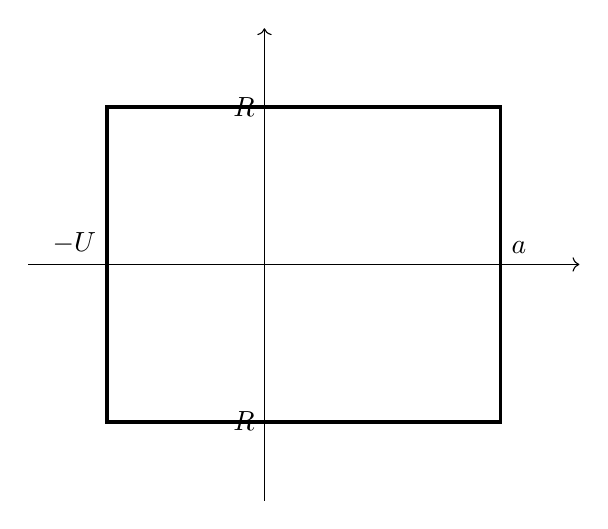
\begin{tikzpicture}
  \draw[->] (-3,0) -- (4,0);
  \draw[->] (0,-3)--(0,-2) node[left]{$-R$} -- (0,2)node[left]{$R$}--(0,3);
  \draw[very thick, black] (-2,-2) -- (-2,0)node[above left, black]{$-U$} -- (-2,2)
    -- (3,2)--(3,0)node[above right, black]{$a$} -- (3,-2) -- cycle;
\end{tikzpicture}
\end{center}
where $U$ is some odd integer. By Cauchy's residue theorem, we have,
\begin{align*}
   {\frac 1 {2\pi i}}\int_{C_R}-{\frac {\zeta'(s)}{\zeta(s)}}{\frac {x^s} s}ds &= \text{sum of residues of ${\frac {\zeta'(s)}{\zeta(s)}}$ in $C_R$},\\
   & = \overbrace{x}^{\text{contribution of poles of $\zeta(s)$}} - \underbrace{{\frac {\zeta'(0)}{\zeta(0)}}}_{\text{contribution of $s=0$}} +\overbrace{\sum_{0<2m<U}{\frac {x^{-2m}} {2m}}}_{\text{contribution of non-trivial zeros of $\zeta(s)$}}-\underbrace{\sum_{\substack{\rho=\beta+i\gamma\\\zeta(\rho)=0\\\vert\gamma\vert<R}}{\frac {x^\rho} {\rho}}}_{\text{contribution of trivial zeros of $\zeta(s)$}}.
\end{align*}
Note that,
\begin{equation*}
  \int_{C_R}=\int_{a-iR}^{a+iR}+\underbrace{\int_{T_1,T_2,T_3}}_{=I}.
\end{equation*}
We then have %specify the equations
\begin{equation*}
  \psi(x) = x-{\frac {\zeta'(0)} {\zeta(0)}}+\sum_{0<2m<U}{\frac {x^{-2m}} {2m}}-\sum_{\substack{\rho=\beta+i\gamma\\\zeta(\rho)=0\\\beta\in(0,1)\\\vert\gamma\vert<R}}{\frac {x^\rho} {\rho}}-I+O\left({\frac {x\log^2x}{R}}\right).
\end{equation*}
\begin{exercise}
  Show that 
  \begin{align*}
    I &= {\frac 1 {2\pi}}\int_{I_1+I_2+I_3}-{\frac {\zeta'(s)}{\zeta(s)}}{\frac {x^s} {s}}ds,
    & = O\left({\frac {x\log^2 R}{R\log x}}+{\frac {R\log U}{Ux^R}}\right).
  \end{align*}
\end{exercise}
Suppose we have above equality, then we have,
\begin{equation*}
  \psi(x) = x-{\frac {\zeta'(0)} {\zeta(0)}}+\sum_{0<2m<U}{\frac {x^{-2m}} {2m}}-\sum{\frac {x^\rho} {\rho}}+O\left({\frac {x\log^2R}{R\log x}}+{\frac {R\log U} {Ux^R}}+{\frac {x\log^2x} R}\right).
\end{equation*}
Recall $U$ is an odd integer. Take $U\to\infty$, we have,
\begin{equation*}
  \psi(x) = x-{\frac {\zeta'(0)} {\zeta(0)}}+\log(1-x^{-2})-\sum_{\rho}{\frac {x^\rho} {\rho}}+O\left({\frac {x\log^2R}{R\log x}}+{\frac {x\log^2x} R}\right).
\end{equation*}
Taking $R\to\infty$, we have,
\begin{equation*}
  \psi(x) = x-{\frac {\zeta'(0)}{\zeta(0)}}+\log(1-x^{-2})-\sum_{\rho}{\frac {x^\rho} {\rho}}.
\end{equation*}
\begin{definition}
  \begin{equation*}
  \psi(x,\chi) \defeq\sum{n\leq x}\Lambda(n)\chi(n).
  \end{equation*}
\end{definition}
Recall we had,
\begin{equation*}
\psi(x,q,a) \defeq\sum_{\substack{n\leq x\\n=a\tmod q}}\Lambda(n),
\end{equation*}
where $(a,q) = 1$. By Theorem \ref{theorem_prime_number_ap}, we have, as $x\to\infty$,
\begin{equation*}
\psi(x,q,a) \sim {\frac {x} {\varphi(q)}}.
\end{equation*}
\begin{exercise}
  Show that for $(a,q)=1$, we have,
  \begin{equation*}
    \psi(x,q,a) = {\frac 1 {\varphi(q)}}\sum_{\chi\tmod q}\psi(x,\chi)\overline{\chi(a)}.
  \end{equation*}
\end{exercise}
\begin{theorem}
  As $x\to\infty$, we have,
  \begin{equation*}
    \psi(x) = x+O(xe^{-c\sqrt{\log x}}),
  \end{equation*}
  where $c>0$ is some constant.
\end{theorem}
\begin{proof}
  Recalling zero free regions of $\zeta$, we have for $s=\sigma+it$, 
  \begin{equation*}
    \sigma>1-{\frac c {\log R}}\Rightarrow\zeta(s) \not=0,
  \end{equation*}
  where $c$ is some constant and $R=\Im(s)$. From this we have,
  \begin{equation*}
    \left\vert\sum_{\vert\gamma\vert<R}{\frac {x^\rho} {\rho}}\right\vert \leq x^{1-{\frac {c} {\log R}}}\sum_{\substack{\rho=\beta+i\gamma\\\zeta(\rho)=0\\\beta\in(0,1)\\\vert\gamma\vert<R}}{\frac 1 {\vert \rho\vert}}<<x^{1-{\frac c {\log R}}}\sum_{\substack{\beta\in(0,1)\\\gamma\in(0,R)\\\zeta(\beta+i\gamma)=0}}{\frac 1 {\sqrt{\beta^2+\gamma^2}}}.
  \end{equation*}
  Set 
  \begin{equation*}
    g(t) = {\frac {1} {\sqrt{\beta^2+t^2}}},
  \end{equation*}
  and 
  \begin{equation*}
    a_t\defeq \sum_{\substack{\beta\in(0,1)\\\gamma\in(0,t)\\\zeta(\beta+i\gamma)=0}}1.
  \end{equation*}
  We now have,
  \begin{align*}
    \sum_{\substack{\beta\in(0,1)\\\gamma\in(0,R)\\\zeta(\beta+i\gamma)=0}}{\frac 1 {\sqrt{\beta^2+\gamma^2}}}& ={\frac {N(R)} {\sqrt{\beta^2+\gamma^2}}}+\int_0^R{\frac {tN(R)} {(\beta^2+\gamma^2)^{{\frac 3 2}}}}dt\\
    & <<{\frac {N(R)}{R}}+\int_0^R{\frac {N(t)} {t^2}}dt,\\
    & = \log R+\int_0^2{\frac {\log t} {t}}+\int_2^R\cdots,\\
    & = \log^2R.
  \end{align*}
  Combining all we get,
  \begin{equation*}
    \left\vert\sum_{\vert\gamma\vert<R}{\frac {x^\rho}{\rho}}\right\vert<<x^{1-{\frac c {\log R}}}\log^2R.
  \end{equation*}
  Choose $\log R = c_2(\log\overline{x})^{{\frac 1 2}}$ we have,
  \begin{equation*}
    \psi(x) = x+O(xe^{-c\sqrt{\log x}}).
  \end{equation*}
  Using Riemann hypotehsis, choose $R= \sqrt{x}$, we then have as $x\to\infty$,
  \begin{equation*}
    \psi(x) = x+O(\sqrt{x}\log^2x)+{\frac {R\log U}{Ux^R}}+{\frac {x\log^2 x}{ R}}.
  \end{equation*}
\end{proof}
\begin{theorem}[Siegel-Walfisz]
  For any $N\in\R$ there is $c_N>0$ such that as $x\to\infty$,
  \begin{equation*}
    \psi(x,q,a) = {\frac x {\varphi(q)}}+O(xe^{-c_N\sqrt{\log x}}),
  \end{equation*}
  where $q\leq (\log x)^N$. This is uniform in $q$. 
\end{theorem}
\begin{exercise}
  Show that Rieman hypothesis is equivalent to that as $x\to\infty$,
  \begin{equation*}
    \psi(x) = x+O(\sqrt{x}\log^2x).
  \end{equation*}
\end{exercise}
\begin{theorem}
  Riemann hypothesis implies that for $(a,q) = 1$, we have, as $x\to\infty$,
  \begin{equation*}
    \psi(x;q,a) = {\frac x {\varphi(q)}}+O(\sqrt{x}\log^2qx).
  \end{equation*}
\end{theorem}
\begin{remark}For $(a,q)=1$, fixed we have as $x\to\infty$.
  \begin{equation*}
    \pi(x,q,a)<{\frac {2x} {\varphi\log {\frac x q}}},q<x.
  \end{equation*}
\end{remark}
\section{Exercise Solutions}
\subsection{Lecture 1 $\sim$ 4}
\begin{exercise}
  Show that 
  \begin{equation*}
    \sum_{n=1}^\infty {\frac {\vert \mu(n)\vert} {n^s}} = {\frac {\zeta(s)} {\zeta(2s)}}.
  \end{equation*}
\end{exercise}
\begin{proof}[Solution.]
  From Theorem \ref{theomre_zeta_inverse}, we have,
  \begin{equation*}
  {\frac 1 {\zeta(2s)}} = \sum_{n=1}^\infty {\frac {\mu(n)} {n^{2s}}}.
  \end{equation*}
  Therefore, we examine,
  \begin{equation*}
    \left(\sum_{n=1}^\infty {\frac {\vert \mu(n)\vert} {n^s}} \right)\left(\sum_{n=1}^\infty {\frac {\mu(n)} {n^s}}\right) = \sum_{n=1}^\infty{\frac 1 {n^s}}\sum_{d|n}\left(\vert \mu(n)\vert\mu\left({\frac n d}\right)\right)
  \end{equation*}
  Note that if $n\not=1$ is not square free, 
  \begin{equation*}
    \vert \mu(n)\vert\mu\left({\frac n d}\right)=0,
  \end{equation*}
  unless $n=k^2$ and $d=k$. If $n$ is square free then by Theorem \ref{mobius_identity}, we have
  \begin{equation*}
    \left(\sum_{n=1}^\infty {\frac {\vert \mu(n)\vert} {n^s}} \right)\left(\sum_{n=1}^\infty {\frac {\mu(n)} {n^s}}\right) = \sum_{n=1}^\infty{\frac {\mu(n)} {n^{2s}}}.
  \end{equation*}
\end{proof}

\begin{exercise}
  Let $\pi(x;z)$ be the number of $n\leq x$ such that it is coprime to all $p\leq z$. Then we have,
  \begin{equation*}
    \pi(x;z)=x\prod_{p\leq z}\left(1-{\frac 1 p}\right)+O(2^z).
  \end{equation*}
\end{exercise}
\begin{proof}[Solution.]
  We have,
  \begin{align*}
    \pi(x;z)&=\sum_{p_1,p_2,\cdots,p_k\leq z}(-1)^{k+1}\left[{\frac{x}{p_1p_2\cdots p_k}}\right],\\
    &=\sum_{p_1,p_2,\cdots,p_k\leq z}(-1)^{k}\left({\frac{x}{p_1p_2\cdots p_k}}-\left\{{\frac{x}{p_1p_2\cdots p_k}}\right\}\right),\\
    & = x\prod_{p\leq z}\left(1-{\frac 1 p}\right)+\sum_{p_1,\cdots,p_k\leq z}(-1)^{k+1}\left\{{\frac{x}{p_1p_2\cdots p_k}}\right\},\\
  \end{align*}
  We have at most $[z]$ primes and there are ${[z]\choose k}$ many ways to pick $k$-many primes. Thus,
  \begin{equation*}
    \left\vert\sum_{p_1,\cdots,p_k\leq z}(-1)^k\left\{{\frac{x}{p_1p_2\cdots p_k}}\right\}\right\vert\leq\sum_{k=0}^{[z]}{[z]\choose k} = 2^{[z]}\leq 2^z.
  \end{equation*}
\end{proof}
\begin{exercise}
  Show that
  \begin{equation*}
    \sum_{p\leq x}{\frac 1 p}\geq \log\log x+c,
  \end{equation*}
  for some constant $c$.
  \label{exercise_1_5_11}
\end{exercise}
\begin{proof}[Solution.]
  Let $\{p_1,\cdots,p_k\}$ be the primes less than $x$, then
  \begin{align*}
    \sum_{l\leq x}{\frac 1 l} & \leq \sum_{\alpha\in\Z_{\geq0}^k}{\frac 1 {\prod p_i^{\alpha_i}}}.\\
    \log [x]&\leq \sum_{l\leq x}{\frac 1 l}.\\
    \Rightarrow \sum_{i=1}^k \log\left({\frac 1 {1-{\frac 1 p}}}\right)&\geq \log\log [x]. \\
    \log p - \log (p-1)&\leq{\frac 1 p}.
  \end{align*}
  We then conclude that 
  \begin{equation*}
    \sum_{p\leq x}{\frac 1 p}\geq \log\log x-1.
  \end{equation*}
\end{proof}
\setcounter{claim}{0}
\begin{exercise}
  Show that 
  \begin{equation*}
    \pi(x)=O\left({\frac x {\log\log x}}\right).
  \end{equation*}
\end{exercise}
\begin{proof}[Solution.]
  \begin{claim}
    We have,
    \begin{equation*}
      -\sum_{p\leq z}\log\left(1-{\frac 1 p}\right) = \sum_{p\leq z}{\frac 1 p}+O(1).
    \end{equation*}
    \label{claim_log_prime_asympt_approx}
  \end{claim}
  \begin{claimproof}
    We have,
    \begin{equation*}
      \log(1-x)=-\sum_{n=0}^\infty {\frac {x^n} n}.
    \end{equation*}
    Thus substituting $x={\frac 1 p}$, we obtain,
    \begin{equation*}
      -\log\left(1-{\frac 1 p}\right)  = {\frac 1 p }+\sum_{n=2}^\infty {\frac 1 {np^n}} \leq {\frac 1 p} +{\frac {{\frac 1 {p^2}}} {1-{\frac 1 p}}} = {\frac 1 p}+{\frac 1 {p^2}}.
    \end{equation*}
    Therefore,
    \begin{equation*}
      -\sum_{p\leq z}\log\left(1-{\frac 1 p}\right) \leq \sum_{p\leq z}{\frac 1 p}+\zeta(2).
    \end{equation*}
  \end{claimproof}
  \par Using $\pi(x,z)$, we have,
  \begin{equation*}
    \pi(x) \leq \pi(x,z)+z = x\prod_{p\leq z}\left(1-{\frac 1 p}\right)+O(2^z)+z.
  \end{equation*}
  Setting $z=\log x$ and using Claim \ref{claim_log_prime_asympt_approx}, we have,
  \begin{equation*}
    \pi(x) \leq x\exp\left(-\sum_{x\leq \log x}{\frac 1 p}+O(1)\right)+O(x^{\log 2}).
  \end{equation*}
  Using Exercise \ref{exercise_1_5_11}, we get,
  \begin{equation*}
    \pi(x) \leq x\exp\left(-\log\log\log(x)+O(1)\right)+O(x^{\log 2}).
  \end{equation*}
  This completes the proof.
\end{proof}
\setcounter{claim}{0}
\begin{exercise}
  Show that 
  \begin{equation*}
    e^{\psi(2n+1)}\int_0^1 x^n(1-x)^ndx,
  \end{equation*}
  is a positive integer and deduce that
  \begin{equation*}
    \psi(2n+1)\geq2n\log 2.
  \end{equation*}
\end{exercise}
\begin{proof}[Solution.]
  \begin{claim}
    For any $n\in\N$, we have,
    \begin{equation*}
      e^{\psi(n)} = \lcm(2,\cdots,n).
    \end{equation*}
  \end{claim}
  Using binomial coefficient, we have,
  \begin{equation*}
    (1-x)^n = \sum_{k=0}^n {n\choose k}(-1)^{k}x^{k}.
  \end{equation*}
  Thus we have,
  \begin{equation*}
    I=\int_0^1 x^n(1-x)^n = \int_0^1\sum_{k=0}^n {n\choose k}(-1)^{k}x^{n+k} = \sum_{k=0}^n (-1)^k{n\choose k}{\frac 1 {n+k+1}}x^{n+k+1}
  \end{equation*}
  Therefore, the first statement follows. For the latter observe that 
  \begin{equation*}
    x(1-x)\leq {\frac 1 4}.
  \end{equation*}
  Therefore,
  \begin{equation*}
    I\leq 2^{-2n}.
  \end{equation*}
  Finally,
  \begin{align*}
    e^{\psi(2n+1)}I\geq1 \Rightarrow e^{\psi(2n+1)}\geq 2^{2n}.
  \end{align*}
\end{proof}

\begin{exercise}
  Let $\chi \tmod q$ be a non-principal character. Then we have,
  \begin{equation*}
    \sum_{n>x}{\frac {\chi(n)} n} = O\left({\frac 1 x}\right).
  \end{equation*}
\end{exercise}
\begin{proof}
  Using Proposition \ref{proposition_abel_summation}, we have,
  \begin{equation*}
    \sum_{n\leq x}{\frac {\chi(n)} n}\leq {\frac {\varphi(q)} x}-\int_1^x {\frac {\varphi(q)} t^2}dt.
  \end{equation*}
  Recall $L(s,\chi)$ is analytic for $\Re(s)>0$, in particular,
  \begin{equation*}
    L(1,\chi)=\sum_{n=1}^\infty{\frac {\chi(n)} n}
  \end{equation*}
  is bounded. Thus we have,
  \begin{align*}
    \sum_{n>x}{\frac {\chi(n)} n}\leq \int_x^\infty {\frac {\varphi(q)} t^2}dt = O\left({\frac 1 x}\right).
  \end{align*}
\end{proof}

\begin{exercise}
  Show that for a non-principal character $\chi\tmod q$, we have,
  \begin{equation*}
    \sum_{n\leq x}\sum_{d\mid n}\chi(d)=xL(1,\chi)+O(\sqrt{x}).
  \end{equation*}
\end{exercise}
\begin{proof}[Solution.]
  \begin{align*}
    \sum_{n\leq x}\sum_{d\mid n}\chi(d)& = \sum_{de\leq x}\chi(d),\\
    & = \sum_{d\leq\sqrt{x}}\chi(d)\left[{\frac x d}\right]+\sum_{e\leq\sqrt{x}}\sum_{\sqrt{x}<d\leq{\frac x e}}\chi(d).\\
    \sum_{\sqrt{x}<d\leq{\frac x e}}\chi(d) & = \sum_{d\leq{\frac x e}}\chi(d)-\sum_{d\leq \sqrt{x}}\chi(d).\\
    \sum_{e\leq\sqrt{x}}\sum_{\sqrt{x}<d\leq{\frac x e}}\chi(d)& \leq 2\varphi(q)[\sqrt{x}]=O(\sqrt{x}).\\
    \sum_{d\leq\sqrt{x}}\chi(d)\left[{\frac x d}\right]& = x\sum_{d\leq\sqrt{x}}{\frac {\chi(d)} d}+O(1),\\
    & = xL(1,\chi)-\sum_{n>x}{\frac {\chi(n)} n}+O(1).
  \end{align*}
  By the previous exercise. We conclude the solution.
\end{proof}

\begin{exercise}
  For non-principal real character $\chi\tmod q$, show that $L(1,\chi)\not=0$.
\end{exercise}
\begin{proof}[Solution.]
  By Lemma \ref{lemma_quadratic_lower_bound}, we have 
  \begin{equation*}
    a_n \defeq \sum_{d|n}\chi(d)\geq0.
  \end{equation*}
  Set 
  \begin{equation*}
    F(x) = \sum_{n\leq x}a_n \chi(d).
  \end{equation*}
  Then by the previous exercise, we have $F(x) = O(\sqrt{x})$. Let 
  \begin{equation*}
    \sum_{n=1}^\infty{\frac {a_n} {n^s}} = s\int_1^\infty {\frac {F(t)} {t^{s+1}}}dt.
  \end{equation*}
  Note that by the definition of Dirichlet series, we have,
  \begin{equation*}
    \sum_{n=1}^\infty{\frac {a_n} {n^s}} = L(s,\chi)\zeta(s).
  \end{equation*}
  $\zeta(s)$ has a simple pole at $s=1$ and $L$ has zero of order at least one at $s=1$, however, 
  \begin{equation*}
    \lim_{s\to 1}s\int_1^\infty {\frac {F(t)} {t^{s+1}}}dt = \infty.
  \end{equation*}
  This is a contradiction.
\end{proof}

\begin{exercise}
  Let $\chi\tmod q$ be a non-principal character then,
  \begin{equation*}
    \sum_{n\leq x}\sum_{d\mid n}\chi(d) = xL(1,\chi)+O(q\sqrt{x}).
  \end{equation*}
\end{exercise}

\begin{proof}[Solution.]
  Previous exercise and $\varphi(q)\leq q$.
\end{proof}

\begin{exercise}
  Show that for $x>1$ and $c>0$, we have
  \begin{equation*}
    {\frac 1 {2\pi i}}\int_{(c)}{\frac {x^s} s}ds = 1.
  \end{equation*}
\end{exercise}
\begin{proof}[Solution.]
  Let $\zeta_c$ be the contour 
  \begin{center}
  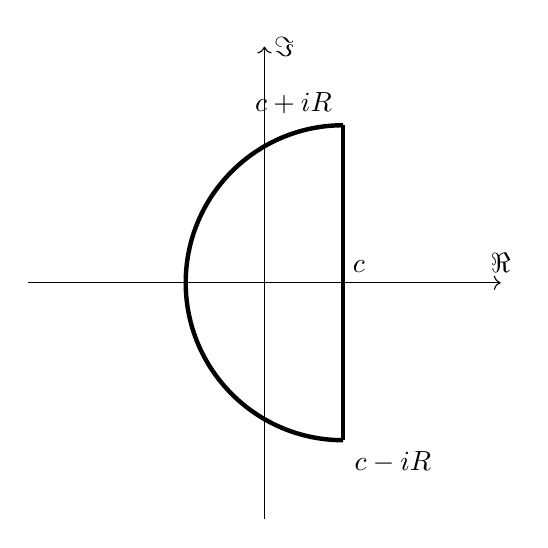
\begin{tikzpicture}
  \draw[->] (-3,0)-- (1,0)node[above right]{$c$} -- (3,0)node[above]{$\Re$};
  \draw[->] (0,-3)--(0,3)node[right]{$\Im$};
  \draw[ultra thick] (1,2)node[above left]{$c+iR$} arc (90:270:2)node[below right]{$c-iR$};
  \draw[ultra thick] (1,2)--(1,-2);
\end{tikzpicture}
\end{center}
going the bold closed path in counterclockwise.  Then 
\begin{equation*}
  {\frac 1 {2\pi i}}\left(\int_{c-iR}^{c+iR}{\frac {x^s} s}ds+x^c\int_{{\frac {\pi} 2}}^{{\frac {3\pi} 2}} {\frac {x^{e^{i\theta}}} {c+e^{i\theta}}}d\theta\right) = \Res_s\left({\frac {x^s} s},0\right) = 1.
\end{equation*}
Let us examine the second term, for some small $\delta>0$,
\begin{align*}
  \left\vert\int_{{\frac {\pi} 2}}^{{\frac {3\pi} 2}}{\frac {x^{Re^{i\theta}}} {c+Re^{i\theta}}}d\theta\right\vert&\leq \int_{{\frac {\pi} 2}}^{{\frac {3\pi} 2}}x^{R\cos\theta}\theta,\\
  & = \left(\int_{{\frac {\pi} 2}}^{{\frac {\pi} 2}+\delta}+\int_{{\frac {\pi} 2}+\delta}^{{\frac {3\pi} 2}-\delta}+\int_{{\frac {3\pi} 2}-\delta}^{{\frac {3\pi} 2}}\right)x^{R\cos\theta}d\theta.\\
  \delta\geq&\int_{{\frac {\pi} 2}}^{{\frac {\pi} 2}+\delta}x^{R\cos\theta}d\theta,\int_{{\frac {3\pi} 2}-\delta}^{{\frac {3\pi} 2}+\delta}x^{R\cos\theta}d\theta.\\
  \int_{{\frac {\pi} 2}+\delta}^{{\frac {3\pi} 2}-\delta}x^{R\cos\theta}d\theta&\leq \pi x^{R\cos\left({\frac \pi 2}+\delta\right)} = \pi x^{-R\sin\delta}\stackrel{R\to\infty}{\to}0.
\end{align*}
As $\delta$ is arbitrary, we conclude the proof.
\end{proof}
\begin{exercise}
  Show that for $x\in(0,1)$ and $c>0$, we have
  \begin{equation*}
    {\frac 1 {2\pi i}}\int_{(c)}{\frac {x^s} s}ds = 0.
  \end{equation*}
\end{exercise}
\begin{proof}[Solution.]
  As in the previous exercise, consider the following contour,
    \begin{center}
  \begin{tikzpicture}
  \draw[->] (-3,0)-- (1,0)node[above right]{$c$} -- (4,0)node[above]{$\Re$};
  \draw[->] (0,-3)--(0,3)node[right]{$\Im$};
  \draw[ultra thick] (1,2)node[above left]{$c+iR$} arc (90:-90:2)node[below right]{$c-iR$};
  \draw[ultra thick] (1,2)--(1,-2);
\end{tikzpicture}
\end{center}
Then,
\begin{equation*}
  {\frac 1 {2\pi i}}\left(\int_{c-iR}^{c+iR}{\frac {x^s} s}ds+x^c\int_{-{\frac {\pi} 2}}^{{\frac {\pi} 2}} {\frac {x^{e^{i\theta}}} {c+e^{i\theta}}}d\theta\right) = 0.
\end{equation*}
Similarly, we observe that 
\begin{equation*}
  \int_{-{\frac {\pi} 2}+\delta}^{{\frac {\pi} 2}-\delta}x^{R\cos\theta}d\theta\leq \pi x^{R\cos\left({\frac \pi 2}-\delta\right)} = \pi x^{R\sin\delta}\stackrel{R\to\infty}{\to}0.
\end{equation*}
\end{proof}
\begin{exercise}
  Show that for $c>0$, we have
  \begin{equation*}
    {\frac 1 {2\pi i}}\int_{(c)}{\frac {1} s}ds = {\frac 1 2}.
  \end{equation*}
\end{exercise}
\begin{proof}[Solution.]
  \begin{align*}
    {\frac 1 {2\pi i}}\int_{c-iR}^{c+iR} {\frac {1} s}ds & = {\frac 1 {2\pi i}}\int_{-R}^{R} {\frac {i} {c+it}}dt,\\
    & = {\frac 1 {2\pi }}\int_{-R}^{R} {\frac {c-it} {c^2+t^2}}dt,\\
  \end{align*}
  Since ${\frac {t} {c^2+t^2}}$ is odd, the imaginary part of the integral vanishes. As ${\frac {1} {c^2+t^2}}$ is even, we consider,
  \begin{align*}
    {\frac 1 {\pi }}\int_0^R{\frac {c} {c^2+t^2}}dt & = {\frac 1 {\pi }}\int_0^{{\frac R c}}{\frac {1} {1+u^2}}du.
  \end{align*}
  As $R$ goes to infinity, the left hand side equals to ${\frac 1 {\pi }}\lim_{u\to\infty}\arctan u={\frac 1 2}$.
\end{proof}
\begin{exercise}
  Show that 
  \begin{equation*}
    M(x)\defeq\sum_{n\leq x}\mu(n) = O(x\exp(-c(\log x)^{{\frac 1 {10}}})),
  \end{equation*}
  for some constant $c>0$.
\end{exercise}
\begin{proof}
  Using Lemma \ref{lemma_partial_sum_integration}, and recall that 
  \begin{equation*}
    {\frac 1 {\zeta(s)}} = \sum_{n=1}^\infty {\frac {\mu(n)} {n^s}},
  \end{equation*}
  we get,
  \begin{align*}
    M(x) & = {\frac 1 {2\pi i}}\int_{(c)}{\frac {x^s} {s\zeta(s)}}ds.
  \end{align*}
  Thus we examine 
  \begin{equation*}
    {\frac 1 {2\pi i}}\int_{c-iR}^{c+iR}{\frac {x^s} {s\zeta(s)}}ds,
  \end{equation*}
  and consider $R\to\infty$.
\end{proof}
\begin{exercise}
  Show that for any $s$ with $\Re(s)=1$, we have,
  \begin{equation*}
    \sum_{n=1}^\infty {\frac {\mu(n)} {n^s}}
  \end{equation*}
  converges.
\end{exercise}
\begin{proof}[Solution.]
  By the assumption, we set $s = 1+it$ for $t\in\R$. Using Proposition \ref{proposition_abel_summation}, we have,
  \begin{equation*}
    \sum_{n\leq N}{\frac {\mu(n)} {n^{1+it}}} = {\frac {O(N\exp(-c(\log N)^{{\frac 1 {10}}}))} {N^{1+it}}}+(1+it)\int_1^x {\frac {M(w)} {w^{2+it}}}dw.
  \end{equation*}
  Examine the splitted integral,
  \begin{equation*}
    \int_1^\infty {\frac {M(w)} {w^{2+it}}}dw-\int_N^\infty {\frac {M(w)} {w^{2+it}}}dw.
  \end{equation*}
  Ther first term conevrges as ${\frac {M(w)} {w^{2+it}}}=O(w^{-1-\delta})$ for some $\delta>0$. Note that 
  \begin{equation*}
    \exp\left(-{\frac c 2}(\log w)^{{\frac 1 {10}}}\right)\leq \exp\left(-{\frac c 2}(\log w)^{{\frac 1 {10}}}\right).
  \end{equation*}
  Thus,
  \begin{align*}
    \left\vert\int_N^\infty {\frac {M(w)} {w^{2+it}}}dw\right\vert & \leq \int_N^\infty\exp\left(-{\frac c 2}(\log w)^{{\frac 1 {10}}}\right)\exp\left(-{\frac c 2}(\log w)^{{\frac 1 {10}}}\right){\frac {dw} w},\\
    & \leq c'\exp\left(-{\frac c 2}(\log N)^{{\frac 1 {10}}}\right)\stackrel{N\to\infty}{\to}0.
  \end{align*}
\end{proof}
\begin{exercise}
  Show that 
  \begin{equation*}
    \sum_{n\leq x}{\frac n {\varphi(n)}}<<O(x).
  \end{equation*}
\end{exercise}
\begin{proof}
  \begin{align*}
    \sum_{n\leq x}{\frac n {\varphi(n)}} & = \sum_{n\leq x}{\frac 1 {\prod_{p|n}\left(1-{\frac 1 p}\right)}},\\
    & = \sum_{n\leq x}\sum_{\gamma(d)|n}{\frac 1 d},\\
    & \leq \sum_{\gamma(d)\leq x}{\frac 1 d}{\frac {x} {\gamma(d)}},\\
    & \leq x\prod_{p\leq x}{\frac 1 {\left(1-{\frac 1 p}\right)}}.
  \end{align*}
\end{proof}
\begin{exercise}
  Show that 
  \begin{equation*}
    \sum_{n\leq x}{\frac 1 {\varphi(n)}}<<\log x.
  \end{equation*}
\end{exercise}
\begin{proof}
  Using the previous problem and Proposition \ref{proposition_abel_summation}, we get,
  \begin{align*}
    \sum_{n\leq x}{\frac n {\varphi(n)}}{\frac 1 n} &\leq {\frac {Cx} x}+C\int_1^x {\frac {t} {t^2}}dt,\\
    & = C+C\log x.
  \end{align*}
\end{proof}
\begin{exercise}
  Prove that 
  \begin{equation*}
    \sum_{n\leq x}{\frac 1 {\varphi(n)}}\sim c\log x.
  \end{equation*}
\end{exercise}
\begin{proof}
  Remains to show that $\log x<<\sum_{n\leq x}{\frac 1 {\varphi(n)}}$.%later
\end{proof}
\begin{exercise}
  Show that for a character $\chi\tmod q$ and $(n,q)=1$, we have,
  \begin{equation*}
    \chi(n)\tau(\overline{\chi}) = \sum_{k=1}^q\overline{\chi}(n)e^{{\frac {2\pi i k n} q}}.
  \end{equation*}
\end{exercise}
\begin{proof}[Solution.]
  Note that we have $\chi(n) = \overline{\chi}(n)^{-1}$. And use 
  \begin{equation*}
    kn\equiv l\mod{q}\Rightarrow k\equiv ln^{-1}\mod{q}.
  \end{equation*}
\end{proof}
\begin{exercise}
  Let $\chi\tmod q$ be a primitive character, then we have,
  \begin{equation*}
    L(1,\chi) = \sum_{n\leq x}{\frac {\chi(n)} {n}}+O\left({\frac {\sqrt{q}\log q} {x}}\right).
  \end{equation*}
\end{exercise}

\begin{proof}
  By Proposition \ref{proposition_abel_summation},
  \begin{equation*}
    L(1,\chi) = \int_1^\infty{\frac {A(t)} {t^2}}dt \Rightarrow \sum_{n>x}{\frac {\chi(n)} {n}}\leq \int_x^{\infty}{\frac {A(t)} {t^2}}dt,
  \end{equation*}
  where 
  \begin{equation*}
    A(x) = \sum_{n\leq x}\chi(n).
  \end{equation*}
  By Theorem \ref{theorem_polya_vinogradov}, we have,
  \begin{equation*}
    \vert A(x)\vert\leq \sqrt{q}\log q.
  \end{equation*}
  Thus we obtain,
  \begin{equation*}
    \int_x^{\infty}{\frac {A(t)} {t^2}}dt \leq {\frac {\sqrt{q}\log q} {x}}.
  \end{equation*}
\end{proof}
\begin{exercise}
  Show that 
  \begin{equation*}
    \sum_{\chi\not=\chi_0}L(1,\chi) = \varphi(q)+O(\sqrt{q}\log q).
  \end{equation*}
\end{exercise}
\begin{proof}
  If $\chi$ is imprimitive, then use Theorem \ref{theorem_polya_vinogradov} to the primitive conductor of it, we obtain the same inequality. Thus 
  \begin{align*}
    \sum_{\chi\not=\chi_0}L(1,\chi) & = \sum_{n\leq x}\left({\frac {\sum_{\chi\not=\chi_0}\chi(n)} {n}}+O\left({\frac {\sqrt{q}\log q} {x}}\right)\right).
  \end{align*}
  Using Remark \ref{cardinality_dirichlet_characters} and Theorem \ref{theorem_sum_character}, furthermore choosing $x=q$ we obtain,
  \begin{equation*}
    \sum_{\chi\not=\chi_0}L(1,\chi) = \varphi(q)\sum_{(n,q)=1}{\frac 1 n}-\sum_{n=1}^q{\frac 1 n}+O(\sqrt{q}\log q).
  \end{equation*}
\end{proof}
\begin{exercise}
  Let $s\in\C$ be such that $\Re(s)=\sigma>0$. Then for any $x$ and a non-trivial character $\chi$, show that
  \begin{equation*}
    L(s,\chi)=\sum_{n\leq x}{\frac {\chi(n)} {n^s}}+O\left({\frac {\vert s\vert\sqrt{q}\log q}{\sigma x^\sigma}}\right).
  \end{equation*}
\end{exercise}
\begin{proof}[Solution.]
  Using Proposition \ref{proposition_abel_summation} and Theorem \ref{theorem_polya_vinogradov}, we have,
  \begin{equation*}
    \sum_{n>x}{\frac {\chi(n)} {n^s}}\leq \vert s\vert \int_x^\infty {\frac {\sqrt{q}\log q} {t^{\sigma+1}}}dt.
  \end{equation*}
\end{proof}
\begin{exercise}
  For $\sigma>{\frac 1 2}$, show that 
  \begin{equation*}
    \sum_{\chi\not=\chi_0}L(\sigma,\chi) = \varphi(q)+O(q^{{\frac 3 2}-\sigma}).
  \end{equation*}
\end{exercise}
\begin{proof}[Solution.]
  By previous exercises, by letting $x=q$, we have
  \begin{equation*}
     \sum_{\chi\not=\chi_0}L(\sigma,\chi) = \varphi(q) + O(q^{1-\sigma})+O(q^{{\frac 3 2}-\sigma}).
  \end{equation*}
\end{proof}
\begin{exercise}
  For a prime $p$ and a quadratic character $\chi$, we have,
  \begin{equation*}
    \tau(\chi) = \begin{cases}
      \sqrt{p},\quad(p\equiv1\mod{p}),\\
      i\sqrt{p},\quad(p\equiv3\mod{p}).
    \end{cases}
  \end{equation*}
\end{exercise}
\begin{proof}
  As $(\Z/p\Z)^\times$ is cyclic, there is a unique quadratic character $\chi$ for each $p$. Let $\zeta_p = e^{{\frac {2\pi i} p}}$. Then 
  \begin{equation*}
    \sum_{k=1}^{p-1} \zeta^k = -1.
  \end{equation*}
  Therefore,
  \begin{equation*}
    \tau(\chi)-1 = \sum_{k=1}^{p-1}(\chi(k)+1)\zeta^k.
  \end{equation*}
  As $\Z/p\Z$ is a field, if an element has square roots then there are exactly two besides $0$. And if $k$ is a square $\chi(k)-1 = 2$ otherwise $0$. Therefore,
  \begin{equation*}
    \tau(\chi)=1+\sum_{k=1}^{p-1}\zeta_p^{k^2}
  \end{equation*}
  Consider,
  \begin{equation*}
    \vert\tau(\chi)\vert^2 = \sum_{k,l=0}^{p-1}\zeta_p^{k^2-l^2} = \sum_{a,b=0}^{p-1}\zeta_p^{ab} = p.
  \end{equation*}
  Remains to prove the parity of this. 
\end{proof}
\end{document}